\documentclass[draftclsnofoot,onecolumn,journal,letterpaper,compsoc,10pt]{IEEEtran}
\usepackage{geometry}
\usepackage{setspace}
\usepackage{titling}
\usepackage{todonotes}
\usepackage{minted}
\usepackage{graphbox}
\usepackage{titlesec}
\usepackage{pdfpages}
\usepackage{pdflscape}
\usepackage{float}
\usepackage{hyperref}
\usepackage{multicol}
\usepackage{adjustbox}

%%%%%%%%%%%%%%%%%%%%%%%%%%%%%%%%%%%%%%%%%%%%%%%%%%%%%%%%%%%%%%%%%%%%%%%%%%%%%%%%%%%%%%%%%%%%%%%%%%%%%%
% DO NOT TOUCH THIS... unless you're careful :) ;] :D
%%%%%%%%%%%%%%%%%%%%%%%%%%%%%%%%%%%%%%%%%%%%%%%%%%%%%%%%%%%%%%%%%%%%%%%%%%%%%%%%%%%%%%%%%%%%%%%%%%%%%%

% Defines \subsubsubsection & \subsubsubsubsection

\titleclass{\subsubsubsection}{straight}[\subsection]
\titleclass{\subsubsubsubsection}{straight}[\subsubsection]

\newcounter{subsubsubsection}[subsubsection]
\renewcommand\thesubsubsubsection{\thesubsubsection.\arabic{subsubsubsection}}

\newcounter{subsubsubsubsection}[subsubsubsection]
\renewcommand\thesubsubsubsubsection{\thesubsubsubsection.\arabic{subsubsubsubsection}}

\titleformat{\subsubsubsection}{\normalfont\normalsize\itshape}{\thesubsubsubsection}{1em}{}
\titlespacing*{\subsubsubsection}{0pt}{3.25ex plus 1ex minus .2ex}{1.5ex plus .2ex}

\titleformat{\subsubsubsubsection}{\normalfont\normalsize\itshape}{\thesubsubsubsubsection}{1em}{}
\titlespacing*{\subsubsubsubsection}{0pt}{3.25ex plus 1ex minus .2ex}{1.5ex plus .2ex}

\makeatletter
\def\toclevel@subsubsubsection{4}
\def\l@subsubsubsection{\@dottedtocline{4}{7em}{4em}}

\def\toclevel@subsubsubsubsection{5}
\def\l@subsubsubsubsection{\@dottedtocline{5}{7em}{4em}}

\makeatother

\setcounter{secnumdepth}{5}
\setcounter{tocdepth}{2}

%%%%%%%%%%%%%%%%%%%%%%%%%%%%%%%%%%%%%%%%%%%%%%%%%%%%%%%%%%%%%%%%%%%%%%%%%%%%%%%%%%%%%%%%%%%%%%%%%%%%%%


\geometry{letterpaper, margin=.75in}
\singlespace

\title{Project Handoff\\\large CS 463 Spring 2018\\Group 19 BrewHops: Ninkasi Brewing, Automating the brewing process}
\author{
    Brennan Douglas \\
    \texttt{douglbre@oregonstate.edu} \\
    \and
    Dan Van Horn \\
    \texttt{vanhornd@oregonstate.edu} \\
    \and
    Henry Peterson \\
    \texttt{peterhen@oregonstate.edu} \\
    \and
    Bailey Singleton \\
    \texttt{singletb@oregonstate.edu} \\
}
\date{May 5th, 2018}

\begin{document}

\begin{titlingpage}
    \maketitle
    \begin{abstract}
        During the 2018-2019 school year, our group has worked on a project with Ninkasi Brewing to write software for tracking data during the beer fermentation process. This is a compilation of our written work from the initial planning stages to reflections after completing the project.
    \end{abstract}
    \pagebreak
    \tableofcontents
\end{titlingpage}

\section{Introduction}
    The Brewhops project was requested by Ninkasi Brewing, based out of Eugene, Oregon. The brewery uses an old school method of tracking their brewing process. Excel spreadsheets being passed through email left Ninkasi wanting a more reliable, single-source site where all tracking information was stored together. The BrewHops application gave them that: a web application that allows for easy tracking and accountability across the entire brewing process. Joe Kleiber was our main client that we communicated with weekly, which allowed us to ask questions at almost any time of day. Constant feedback from Joe was critical to our success, as the BrewHops members could make decisions based directly off of the client's specifications. The members of the BrewHops team included Bailey Singleton, Dan Van Horn, Brennan Douglas, and Henry Peterson. Working off of a previous project started by a capstone team of the year prior, gave us a good starting point while also allowing us freedom to change the application to something better and more user friendly. 
    % Who requested it?
    % Why was it requested?
    % What is its importance?
    % Who was/were your client(s)?
    % Who are the members of your team?
    % What were their roles?
    % What was the role of the client(s)? (I.e., did they supervise only, or did they participate in doing development)


\newpage
\section{Requirements Document}
{
    \let\section\subsubsection
    \let\subsection\subsubsubsection
    \let\subsubsection\subsubsubsubsection
    \section{Introduction}

This document will lay out the technical specifications for the completion of the Ninkasi project.  It will outline uses cases for new features, and features that need to be repaired or updated.  In total, this document will detail all that needs to be done in order for the automated brewing project to be considered complete.

    \subsection{System Purpose}

    The purpose of the automated brewing project is to make a more sustainable system for Ninkasi to track, store, and visualize the data associated with the brewing of their beer.  As it stands there is already an application that has a working database that models the data needed by Ninkasi and has some rudimentary pages to display and enter this data.  Our extension on the system has the purpose to improve on the existing application in all manner.
    
    Upon completion the application should allow users to enter data for a given beer batch on a mobile device.  This data will then be automatically added to a set of graphs to help visualize the stage at which the specific batch is through its life cycle.  The application will track all data history associated with these batches, the tanks, they are in, and the brand they are a part of.  This will allow deep analytic looks into the brewing process over years worth of data.
    
    \subsection{System Scope}
    
    The system stores all the data, both current and past, associated with each batch of beer that Ninkasi brews.  This is stored in a database.  The web application serves two purposes: to manage the data, and to display the data.  As data management is concerned this means adding and updating data.  Along with this will be a concept of user roles, so a basic login and security system is set in place.  An extension that this project adds is the importing of data from their alkalizer machine, in the form of CSV files.  This project also adds new forms of data visualization.  Specifically new graphs that represent the data in new light.  The final thing that this iteration on the application brings is an upgrade of the technologies being used to bring them to modern standards.  These are broken down into three epics:
    
    \begin{itemize}
        \item Maintenance 
        \item Data Flow
        \item User Interface
    \end{itemize}
    
    \subsection{System Overview}
    
        \subsubsection{System context}
        Previously Ninkasi was using large ever expanding excel spreadsheets to keep track of all of their data.  This single spreadsheet would be passed around by email to different people who would add data and make edits to newly entered data.  As their operation grew larger this has become more and more cumbersome and prone to errors.
    
        \subsubsection{System functions}
        The system stands to improve this process via the web application.  As the current application stands it isn't production ready.  Thus the Maintenance epic will fix this by improving and fixing different features while creating a more complete docker-ized version of the application.  From there the Data Flow through, mainly into, the application will be improved by adding some new features to allow quicker data entry.  Finally, the User Interface will be improved to allow for easier use and better understanding of the website.
        
        \subsubsection{User characteristics}
        There are two sets of users: the admin and the standard user.  The admin will be able to manage all other users and every faucet of the applications data.  They will be on par with a manger who is overseeing the brewing process for a particular brand, or more than one.  The standard user will then be the tester two makes the measurements on each batch and inputs the data.  They will be able to enter data and see the visualizations but won't have much control over the application.
        
        The user of this application, Ninkasi, is looking for it to be a streamlined data entry and visualization process.  It needs to be easy to use when a desktop computer isn't available as most of the data will be entered via a tablet carried around in one of their warehouses.  Past that they are looking for some parts of the process to be automated as well given how repetitive they are.

    \subsection{Definitions}
    \begin{itemize}
        \item We --- refers to our team name BrewHops
        \item Epic --- a big chunk of work that has one common objective.
        \item User Story --- a simple description of a software feature from an end-user perspective.
        \item Agile Software Development --- an approach to software development under which requirements and solutions evolve through the collaborative effort of self-organizing and cross-functional teams and their customer(s)/end user(s)
        \item Docker --- a container platform for normalizing the application's run-time environment \cite{docker}
        \item Kubernetes --- a container (e.g. docker) scripting platform \cite{kubernetes}
        \item K8 --- shorthand for Kubernetes
        \item React --- the web framework that the project uses \cite{react}
        \item TypeScript --- a typed version of JavaScript \cite{typescript}
    \end{itemize}

\section{System Requirements}
    \subsection{Functional Requirements}
    The function of the system is to track all of the brewing data that is currently tracked via excel spreadsheets. This data will be managed by form entry on a website and by an automated upload process.
    \subsection{Usability Requirements}
    The system must have a user friendly interface that is easy to navigate and needs little direction on how to use. There should be little chance for a user to make a mistake and all user input should have helpful validation messages.
    \subsection{System Security}
    Only authenticated users will be able to log into the system and view or make changes. This will be managed by JSON web tokens which will validate each request and all user input will be sanitized before sending it back to the server.
    \subsection{Information Management}
    The data will be stored in a PostGreSQL database running inside of a virtual machine. We will have redeploy scripts and and an archival process by which no data will be lost.
\section{Software Development Requirements}
        The software development requirements are organized into epics and further into user stories. As we will be adhering to agile software development methods, the layout of this section most accurately represents what work will be completed and how it will be organized. Each "story" is written in the context of the party to whom the task benefits.
    \subsection{Maintenance}
        \subsubsection{Login process}
        The login process for the application is not working currently and there are currently only administrator roles available. As a user, there must be a secure way to log into the system and there must be appropriate administrator and non-administrator privileges assigned to each employee. As a developer, I would like to be sure that only authorized users are using our system, so that it stays secure. 
        \subsubsection{Track edits}
            Currently, there is no way for anyone using the database to be held accountable for making changes or adding data. As a user or scientist, I want to be able to see a history of changes to a fermenter, batch, or brand so that I can be sure that the correct information is being updated. This way, all changes are saved and can be reverted, if an error is made. 
        \subsubsection{Language conversion}
            The web application is written in Javascript, which is not a type-safe language, and would like to use a more strict language for writing the code.
            As a developer, I would like to use a language that provides strict typing, to create an easier development cycle and faster debugging. As a user, I would appreciate using a more type-forward language as it makes the developers happy.
        \subsubsection{Create test suites}
            There is no testing on the current application, which makes it hard to tell if the application is running as specified. As a developer, I would like to implement a test suite, so that we can be sure we are delivering proper code. As a user, I would like a test suite, so that I can know all of my specifications are being met to the fullest. 
        \subsubsection{Deployment}
            The current application is being hosted on a Oregon State web server space. We would like to change to have it be something reliable, and that can handle lots of traffic if necessary. As a developer, I would like to deploy the web server on a Docker container on a proper URL so that the site runs smoothly. As a Ninkasi user, I would like to have the application on a dedicated website, as it is more professional and will not be taken down when the current student graduates.        
    \subsection{Data Flow}
        \subsubsection{Review current database schema}
        The schema of the database does not accurately represent the data we want to track right now. As a developer, I need a consistent database schema that meets all of Ninkasi's needs and is easy to interact with. New tables will need to be added and current tables will be edited to make sure we are representing each relationship correctly.
        \subsubsection{Automate data import}
        The alkalizer machine, which takes samples from the fermenters daily, outputs this data into CSV spreadsheet files. As a brewer, I want to automatically upload this data into the system eliminating the need for manual data entry. This task will likely be done with a python script and automatically import the new data into the database.
        \subsubsection{Track history by tank and batch}
        As a brewer I want to track the history of each batch that has been brewed in each fermenter. I also want to track the history of each batch that has been brewed by recipe. The database will be updated to reflect this relationship in such a way that the API and app can easily retrieve and display it.
        \subsubsection{Track fermentation curve data}
        As a brewer, I want to track the data that is used to generate fermentation curves for each tank. The database will be updated to track this data.
    \subsection{User Interface}
        \subsubsection{Improve tank status display}
        The tank status display on the homepage does not meet usability standards. As a user I want to see a compact view of each tanks status when I log in. When I click on a tank, I want navigate to the tank page. 
        \subsubsection{Add new graphic visualizations}
        The fermentation curves are hosted on a separate application that pulls from a different data source. As a user, I would like this information consolidated so I only have to go to one place. The application that generates fermentation curves will be migrated to the source code of this application. It may have to be re-written in a different language but the existing logic will provide the scaffolding. 
        \subsubsection{New history pages}
        The current application only displays the history of each batch. As a user, I want to see the history of each batch brewed per tank and the batch history per brand or recipe. Additional pages are needed and each must link to the current batch history if the batch is clicked.  
        \subsubsection{New options in administrator view}
        In the administrator page, there is only an option to add a user account. There is no way to manage users or their passwords. As a system administrator I want to have more control over who can use the system as well as manage user accounts more effectively. 

\section{Verification}
    \subsection{Maintenance}
        \subsubsection{Login process}
            The testing suite will run a series of inputs into the login system. It will be complete when it rejects unregistered users, gives access to regular users, and gives extra access to administrative users.
        \subsubsection{Track edits}
            This will be complete when every edit is stored in the system and the times are accurately tracked.
        \subsubsection{Language conversion}
            This will be complete when there is no more Javascript code that is able to be converted to the the target language. This should not affect the functionality of the application.
        \subsubsection{Create test suites}
            The testing suites for the front-end and the back-end will be complete when at least 80\% coverage is reached for statement, branch, and function coverage over entire code body.
        \subsubsection{Deployment}
            The deployment system will be complete when both the server and the main application can be successfully started. The employees at Ninkasi must also be confident that they can carry out the procedure as well.
    \subsection{Data Flow}
        \subsubsection{Review current database schema}
            This will be complete when the database accurately represents our full ER diagram for the system.
        \subsubsection{Automate data import}
            The import process will be finished when a CSV file from the alkalizer can be uploaded, and be accurately represented in the database.
        \subsubsection{Track history by tank and batch}
            This will be complete when there are database elements for tanks, brands, and batches.
        \subsubsection{Track fermentation curve data}
            This will be complete when the data that is pulled out by hand to generate fermentation curve graphs can be automatically gathered.
    \subsection{User Interface}
        Determining when user interface requirements are complete depends largely on user feedback. The people who will be using the application must be satisfied that interface is useful and intuitive in addition to it handling at least every function the current system supports. Once they give the OK on feel, these items will be complete.
        \subsubsection{Improve tank status display}
            The tank status page will be complete when the data is displayed in an organized format and no work-arounds are required to view the desired information.
        \subsubsection{Add new graphic visualizations}
            The graphic visualizations will be complete when the graphs currently generated in shinyapps.io can be displayed and easily accessed within the application.
        \subsubsection{New history pages}
            The history section will be complete when there are pages that contain all of the previous information about tanks and brands.
        \subsubsection{New options in administrator view}
            This will be complete when an administrator can add, edit, and delete users.

\section{Gantt Chart}
\begin{center}
    \makebox[\textwidth]{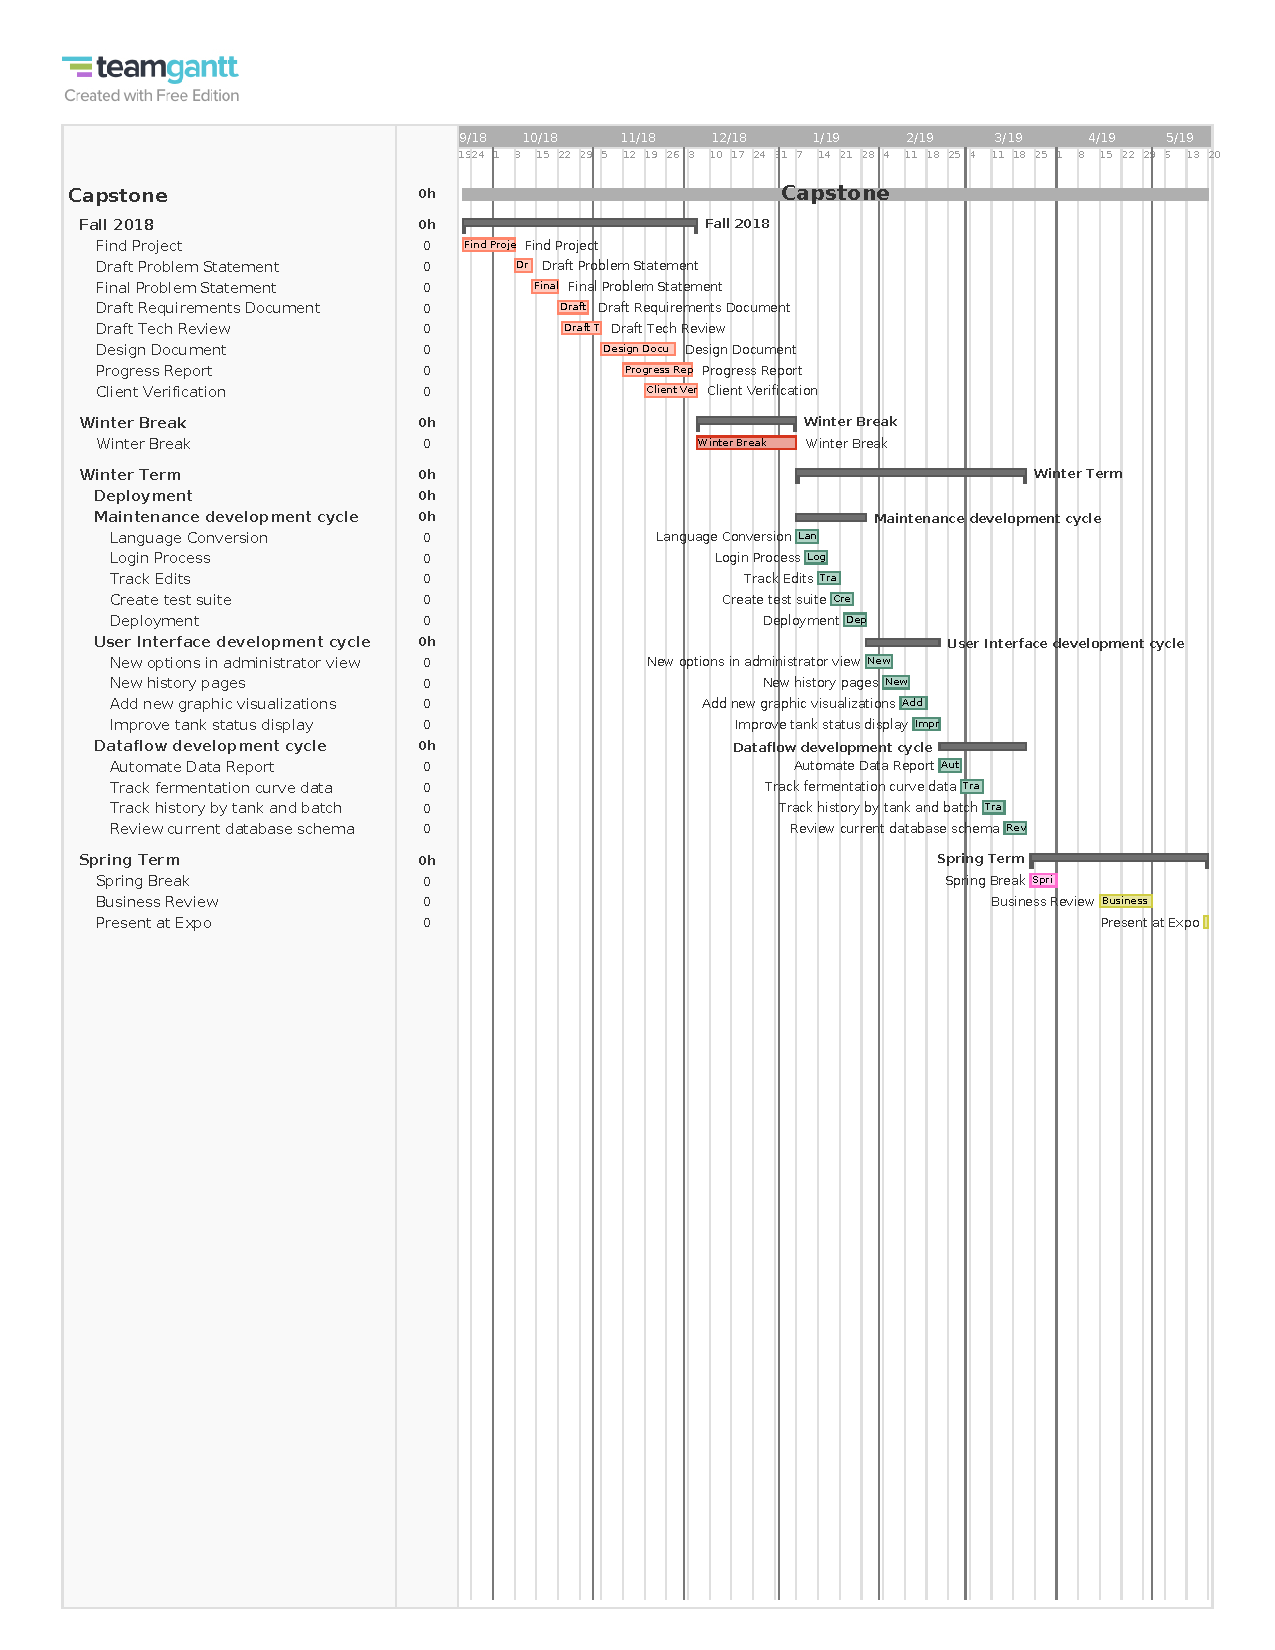
\includegraphics[clip, trim=0cm 11cm 0cm 0cm, width=1.0\paperwidth]{diagrams/gantt.pdf}}
\end{center}
}

\newpage
\section{Design Document}
{
    \let\section\subsubsection
    \let\subsection\subsubsubsection
    \let\subsubsection\subsubsubsubsection
    \section{Introduction}

The design for the Ninkasi Brewhops application is outlined based upon the requirements that have been laid out. The application includes four major components that will be broken down in the following way: database, front-end, API, and dev-ops. The technologies chosen for the design expand on those chosen in the technology reviews that have been conducted for each software component.

    \subsection{System Purpose}

    The purpose of the automated brewing project is to make a more sustainable system for Ninkasi to track, store, and visualize brewing data.  As it stands, there is an existing application that has a working database that models the data needed by Ninkasi. The app has some rudimentary pages to display and enter this data.  Our extension on the system will improve upon this and add new features.
    
    Upon completion, the application will allow users to enter data for a given beer batch on a mobile or desktop device. The data will then be automatically added to a set of graphs to help visualize the lifecycle of a specific batch. The application will track all data history associated with these batches, the tanks they are in, and the brand they are a part of. This will allow deep analytic looks into the brewing process over years worth of data.
    
    \subsection{System Scope}
    
    The system currently stores all the data associated with each batch of beer that Ninkasi brews in a relational database.  The web application serves two purposes: to manage the data (add and update), and to display the data.  Along with this there is a concept of user roles, so a basic login and security system is set in place.  An extension that this project adds is importing data from Ninkasi's alcolyzer (alcohol content analyzer), in the form of CSV files.  This project also adds new forms of data visualization.  Specifically, a graph that shows the fermentation curves for each batch. Finally, the technologies being used will be upgraded to bring them to modern standards.  These are broken down into three epics:
    
    \begin{itemize}
        \item Maintenance 
        \item Data Flow
        \item User Interface
    \end{itemize}
    
    \subsection{System Overview}
    
        \subsubsection{System context}
        Previously, Ninkasi was using large ever expanding excel spreadsheets to track their data brewing data.  This single spreadsheet would be passed around by email to different people who would add data and edit data. With the growth of the business, it has become much more cumbersome and error prone.
    
        \subsubsection{System functions}
        The system stands to improve this process via the web application.  The current application is not production ready and reaching that point will be the foremost goal during the Maintenance epic. During that phase, a more complete docker-ized version of the application will be developed and reported bugs will be fixed.  The Data Flow through the application will be improved by adding new features to allow quicker data entry. Finally, the User Interface will be improved to allow for easier use and better understanding of the website.
        
        \subsubsection{User characteristics}
        There are two types of users: administrators and standard users.  The admin will be able to manage all other users and every facet of the application data. They will be on par with a manager who is overseeing the brewing process for a particular brand, or more than one.  The standard user will be the tester who makes the measurements on each batch and inputs the data.  They will be able to enter data and see the visualizations but won't have much control over the application.
        
        Ninkasi wants a streamlined data entry and visualization process.  It needs to be easy to use when a desktop computer isn't available.  Most of the data entry will be performed via a tablet.  Finally, they want parts of the process to be automated.

    \subsection{Definitions}
    \begin{itemize}
        \item We --- refers to our team name BrewHops
        \item Epic --- a big chunk of work that has one common objective.
        \item User Story --- a simple description of a software feature from an end-user perspective.
        \item Agile Software Development --- an approach to software development under which requirements and solutions evolve through the collaborative effort of self-organizing and cross-functional teams and their customer(s)/end user(s)
        \item Dev-Ops --- Development Operations, a set of practices that automates the processes between software development and IT teams, in order that they can build, test, and release software faster and more reliably.
        \item Docker --- a container platform for normalizing the application's run-time environment \cite{docker}
        \item Kubernetes --- a container (e.g. docker) scripting platform \cite{kubernetes}
        \item K8s --- shorthand for Kubernetes
        \item Vue --- the web framework that the project uses \cite{react}
        \item TypeScript --- a typed version of JavaScript \cite{typescript}
        \item Microservices --- a variant of the service-based architecture where software components are loosely coupled and small.
        \item Relational Database --- a database structured to recognize relations among stored items of information
        \item Application Programming Interface (API) --- a system of software tools and resources that enables developers to create applications 
        \item Single File Component (SFC) --- a file for web development that contains markup, functionality, and styling code.
        \item Single Page Application (SPA) --- an app that loads a single HTML page and dynamically changes that page as the user interacts with the app
    \end{itemize}

\section{System Architecture}
\begin{figure}[H]
    \centering
    \caption{The system architecture for Ninkasi Brewhops}
    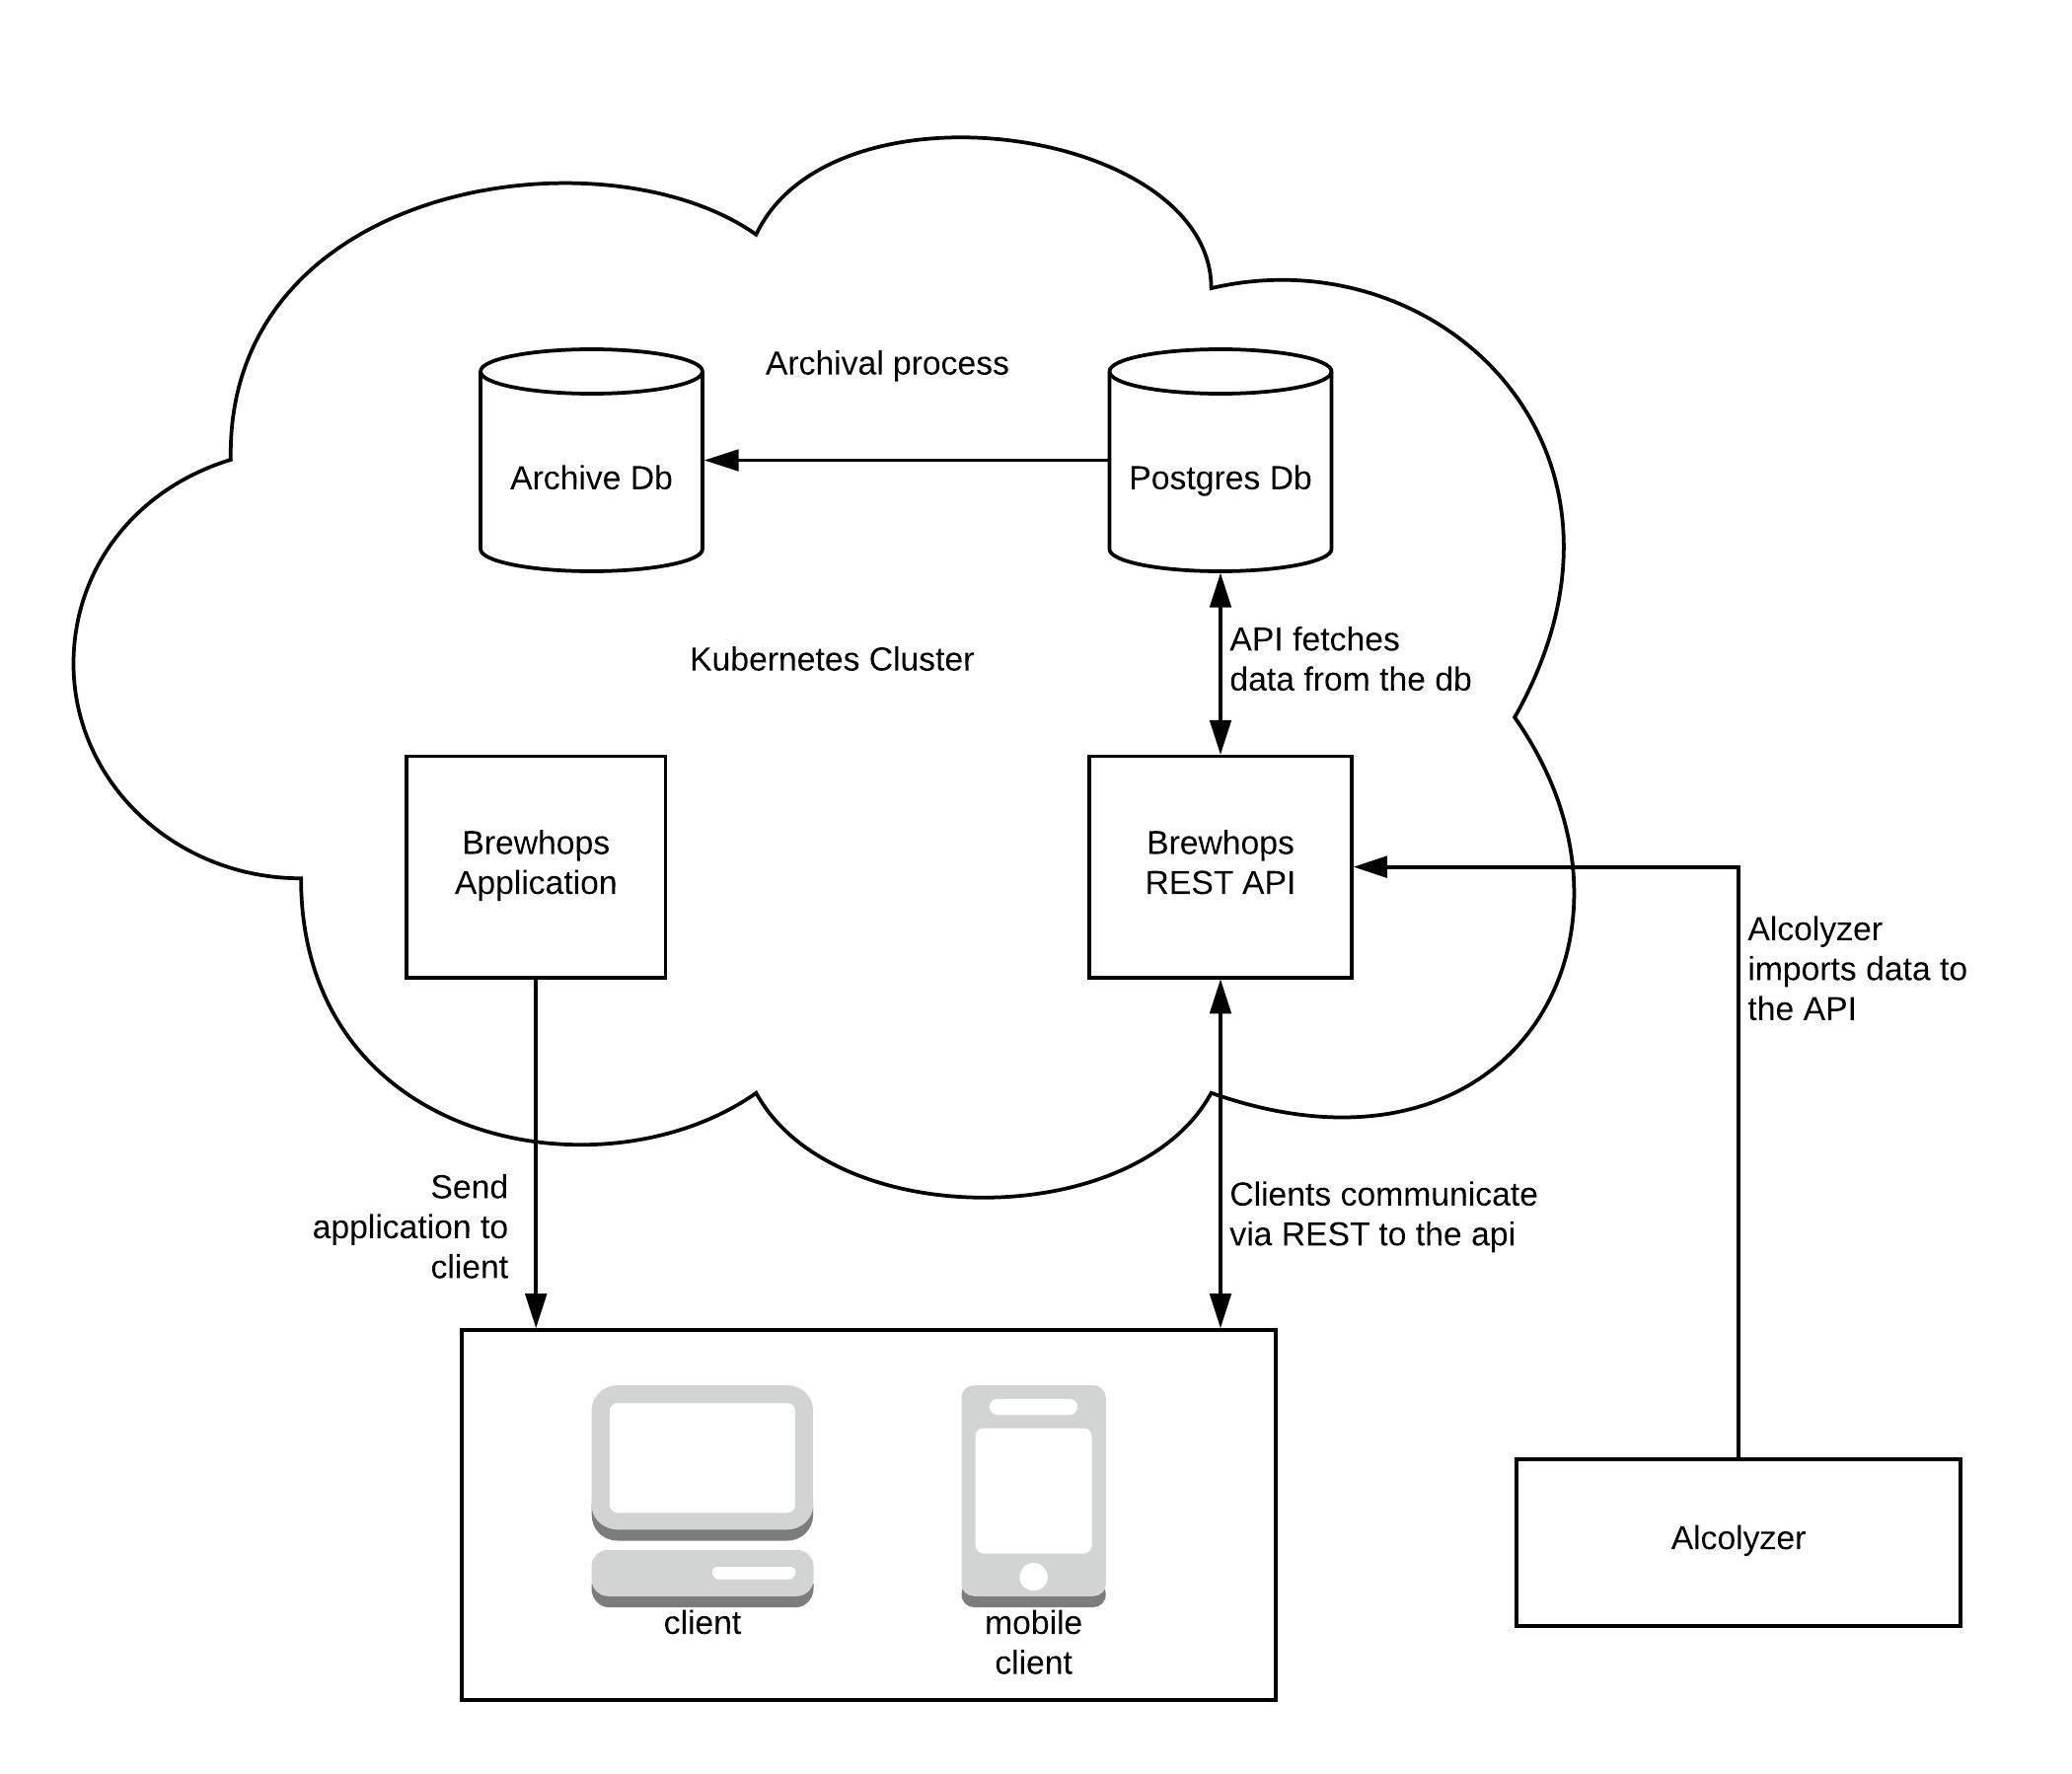
\includegraphics[origin=c,width=0.8\textwidth,keepaspectratio]{./diagrams/brewhops-architecture.jpeg}
    \label{System Architecture}
\end{figure}

The BrewHops system is designed with microservice architecture, a variant of the service-based architecture. The three main software components, front-end, API, and database, are loosely coupled and do not rely on each other to run. Individual teammates will be able to develop and scale these pieces without fear of effecting other work.

The front-end is only responsible for asking the API for data and displaying it. If the data needs to change the front-end will pass that work onto the API. The API is the liaison between the front-end and database. It can create, read, update and delete data from the database. The database itself is only responsible for storage. The BrewHops team has experience designing microservice systems from industry. The reason that the team has chosen this pattern is because of its compatibility with cloud hosting services and simplicity rather than combined team experience. 
\section{Design}

    \subsection{Database}
    
    This section lays out the design of the database.  It includes all changes that need to be made to the current schema to account for the software requirements that have been laid out.
    
        \subsubsection{Existing}
        The existing database already has the core entities that are needed to keep track of all of the required information.  The different batches of beer, their version measurements, recipes, and tanks (the containers that the batches are brewed in) all already exist.  Different entities for providing a rudimentary task system also exist, these include: Tasks, Actions, and Employees.  The employee entity also represents the user object with user name and password fields.  The layout of the database can be seen in the ER diagram at figure \ref{erd}.
        
        \begin{figure}
            \centering
            \caption{ER diagram for the existing database schema.}
            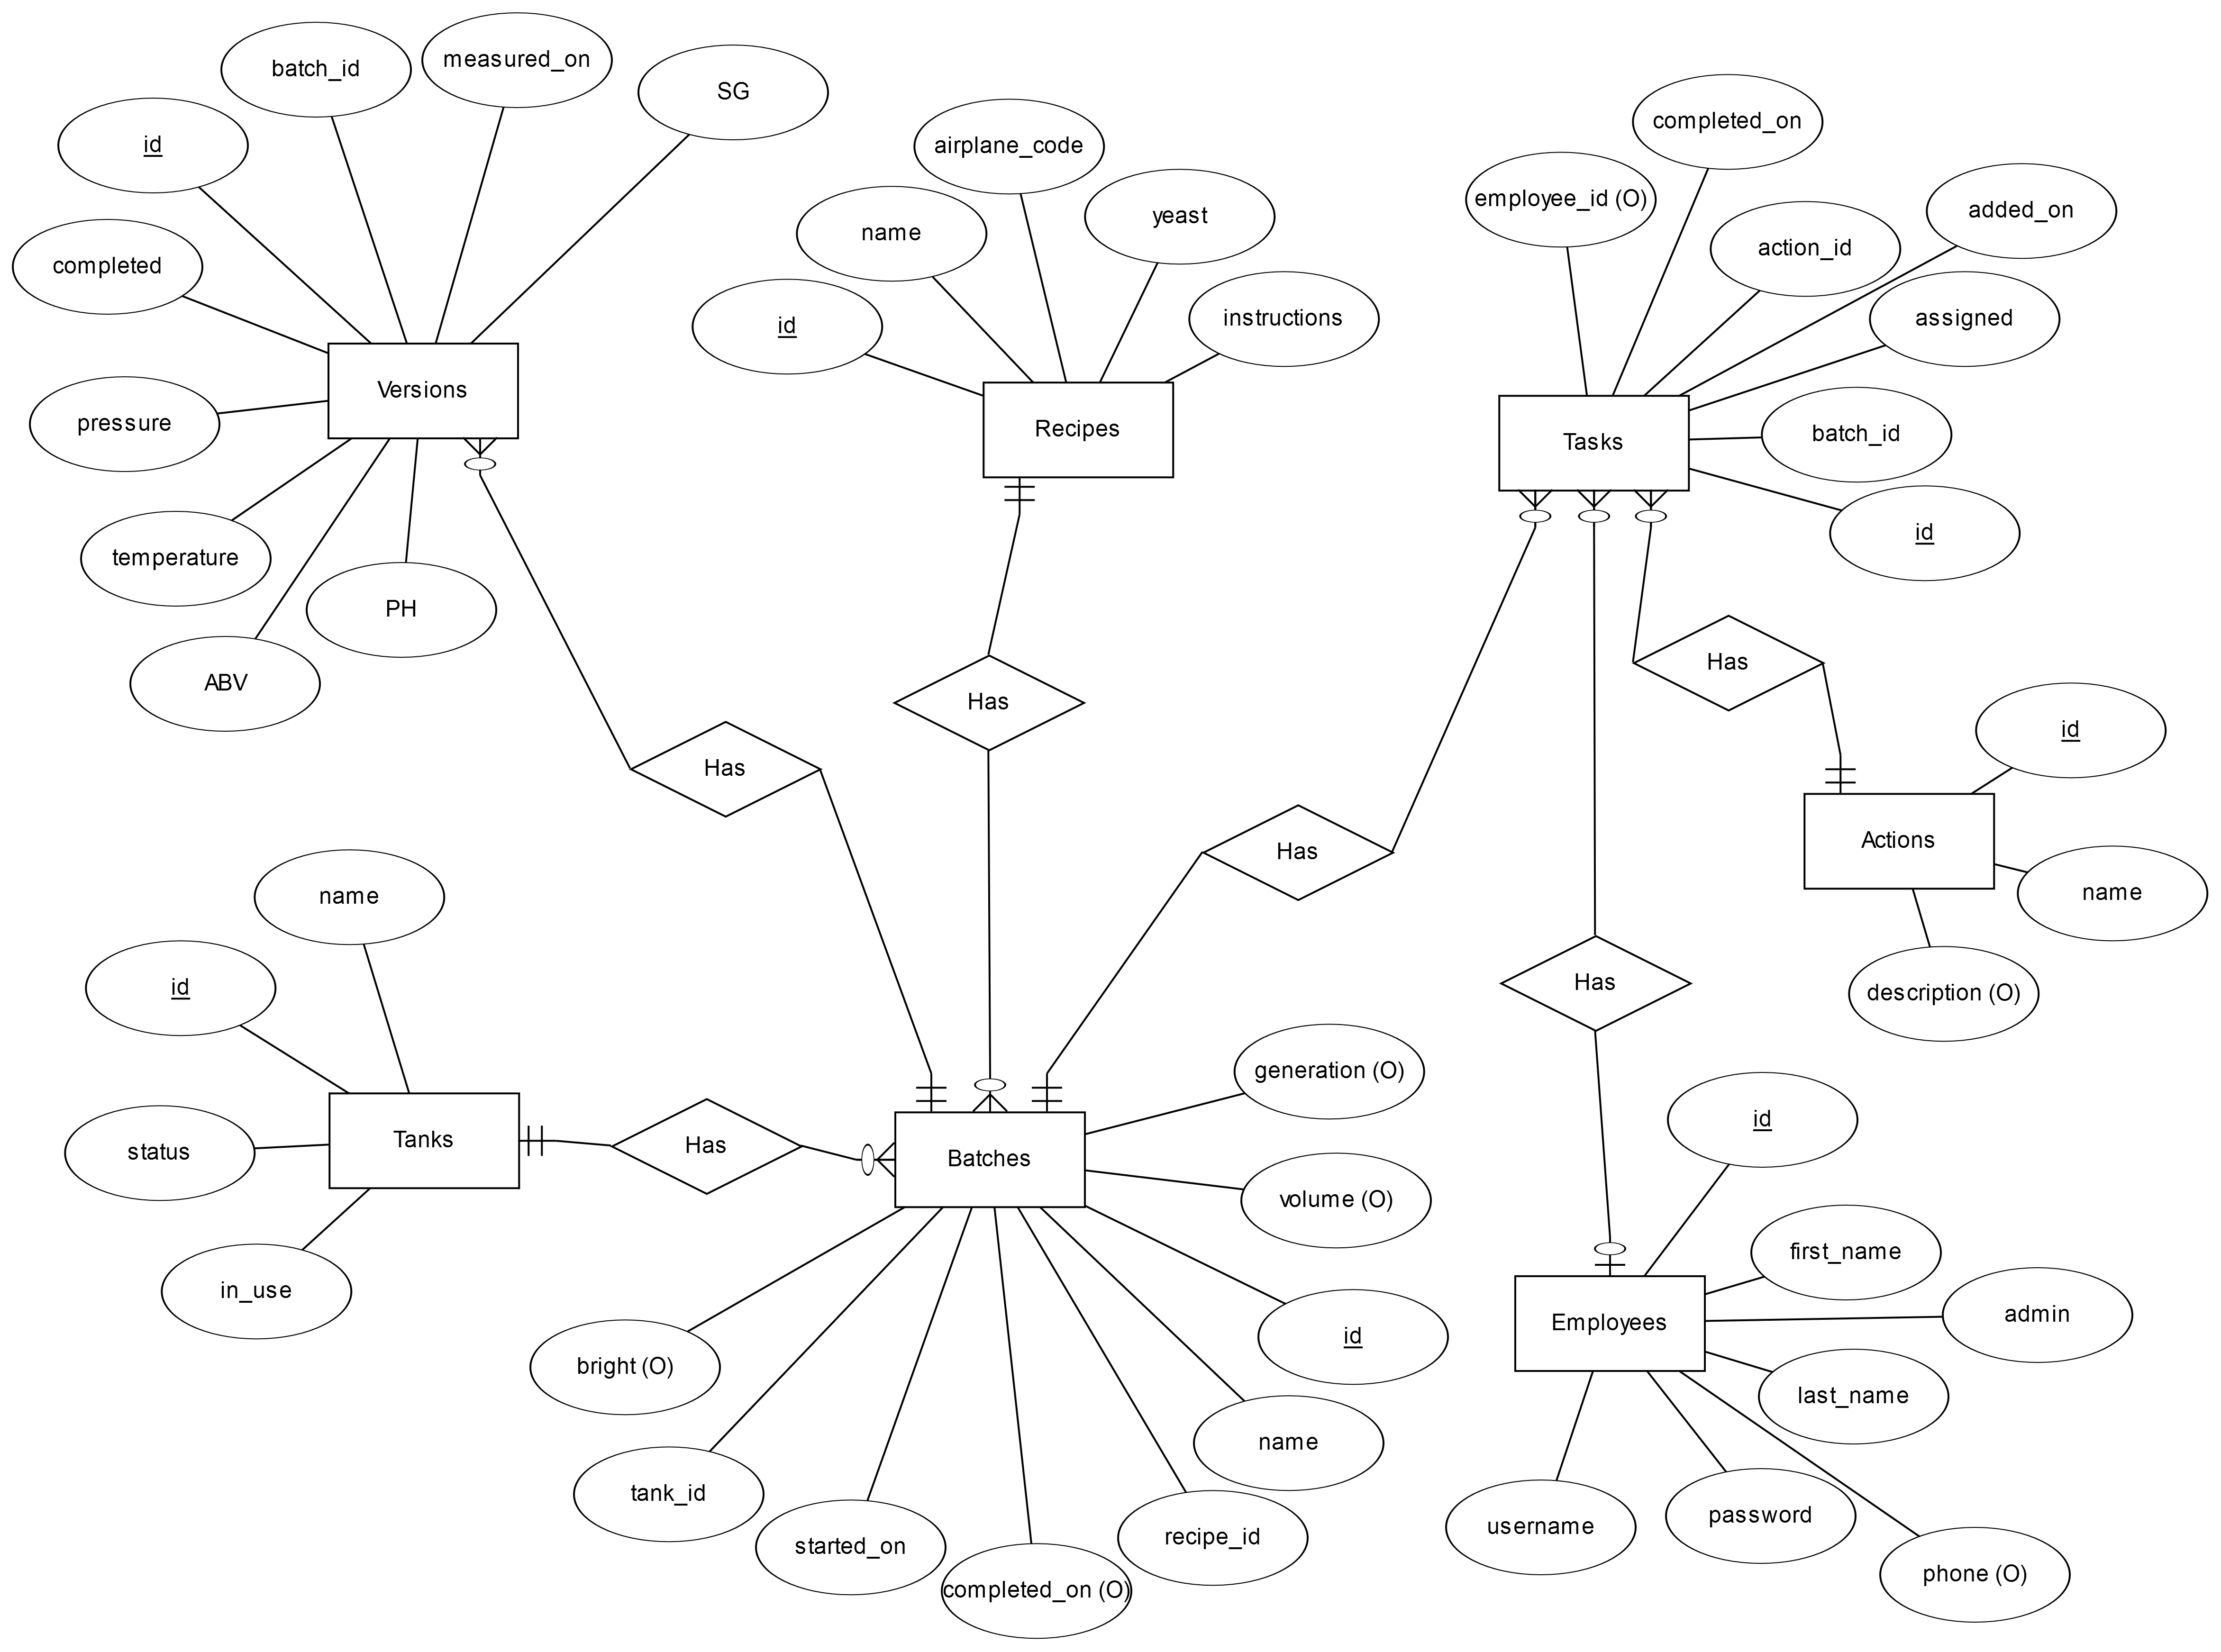
\includegraphics[angle=90,origin=c,width=\textwidth,keepaspectratio]{./diagrams/erdplus-diagram.png}
            \label{erd}
        \end{figure}
    
        \subsubsection{Updates}
        First, security needs to be updated.  Plain text passwords shouldn't be kept in the database as it is major security vulnerability. To resolve this, the password attribute on Employee will be converted into a password hash.  Upon log in, the given password can be hashed again and compared against the stored hash.  This still allows the user to log in but no longer stores their password in plain text.
        
        Next, new functionality defined by the requirements document requires some additions.  Every edit that is made to one of the tables needs to be tracked so that they can be audited.  The person who made the changes also needs to be tracked.  To accomplish this auditing every table will have a "last\_updated\_by" column added to it which will hold the id of the Employee entity who last updated that row.  The edits will then be kept track of by implementing "shadow" tables for each entity.  A shadow table is a table that is exactly identical to the table schema it is "shadowing".  The shadow table makes a new row every time a change occurs to its counter part.  The action associated with this change is tracked (e.g. insert, update, and deletes) and the previous/updated values are stored in the new row (which contains a reference to the row that was changed).  These shadow tables' naming schema will match the name of their respective table with "\_history" appended onto it.  These shadow tables will be implemented with trigger on each of the possible actions: insert, update, delete.
        
        An example of an updated table definition with a shadow table is:\\
        
        \begin{minted}[
            xleftmargin=18pt,
            linenos,
            autogobble,
            breaklines,
        ]{sql}
            CREATE TABLE IF NOT EXISTS recipes (
                id              SERIAL      NOT NULL PRIMARY KEY,
                name            VARCHAR(30) NOT NULL,
                airplane_code   VARCHAR(50) NOT NULL,
                yeast           INT         NULL,
                instructions    JSONB       NOT NULL,
                last_updated_by SERIAL      NOT NULL
            );
            
            CREATE TABLE IF NOT EXISTS recipes_history (
                id              INT         NOT NULL PRIMARY KEY,
                recipe_id       SERIAL      NOT NULL,
                name            VARCHAR(30) NOT NULL,
                airplane_code   VARCHAR(50) NOT NULL,
                yeast           INT         NULL,
                instructions    JSONB       NOT NULL,
                last_updated_by SERIAL      NOT NULL
            );
        \end{minted} 
    
        Here a new column was added to the recipe table, "last\_updated\_by" that will hold the id of the last employee to update the row.  Then the shadow table, "recipes\_history", was created.  The id represents the id of the shadow table and the id that represents the recipes id has been moved to "recipe\_id".  Foreign key relationships on these ids have purposely been left off as it causes issues when every table has a reference to one other one.  And there is no foreign key for the shadow table's reference to the recipe row as when the row gets deleted it will no longer exist but the shadow table should still hold the data.
    
    \subsection{Front-end}
    \subsubsection{View}
    The front-end application will aim to be as light as possible and rely on the external API rather that its own server to authenticate users and access data. It will be written in Vue.js, taking advantage of the single file component (SFC) pattern. An SFC file contains three sections: the view template, logic, and styling. This is contrary to traditional web design where those three sections, namely HTML, CSS, and JavaScript, were largely separated into their own files. 

    The app will be a single page application (SPA) that will simply switch out SFCs when the user navigates to different pages. The main page component will render its sub-components, also SFCs, preserving separation of concerns. Data and functionality will flow through the application from the top down, as shown in figure 3. This means that any data a component needs to render itself will be passed through by its parent. Additionally, if the parent needs to perform some action based on its child component, a function is passed to the child that it can call to notify its parent.
    
    \subsubsection{Communication}
    A client interface will be defined to encapsulate the logic for communication with the API. With TypeScript we can define the types that will be returned by the interface, apply static type-checking to it, and by extension to the whole application. The static type-checking will greatly decrease the development time of the front-end and eliminate time spent tracking down data-based bugs. All error handling will be taken care of inside the interface, so view logic remains simple.
    
    \begin{figure}[H]
        \centering
        \caption{Example of the data flow through view components}
        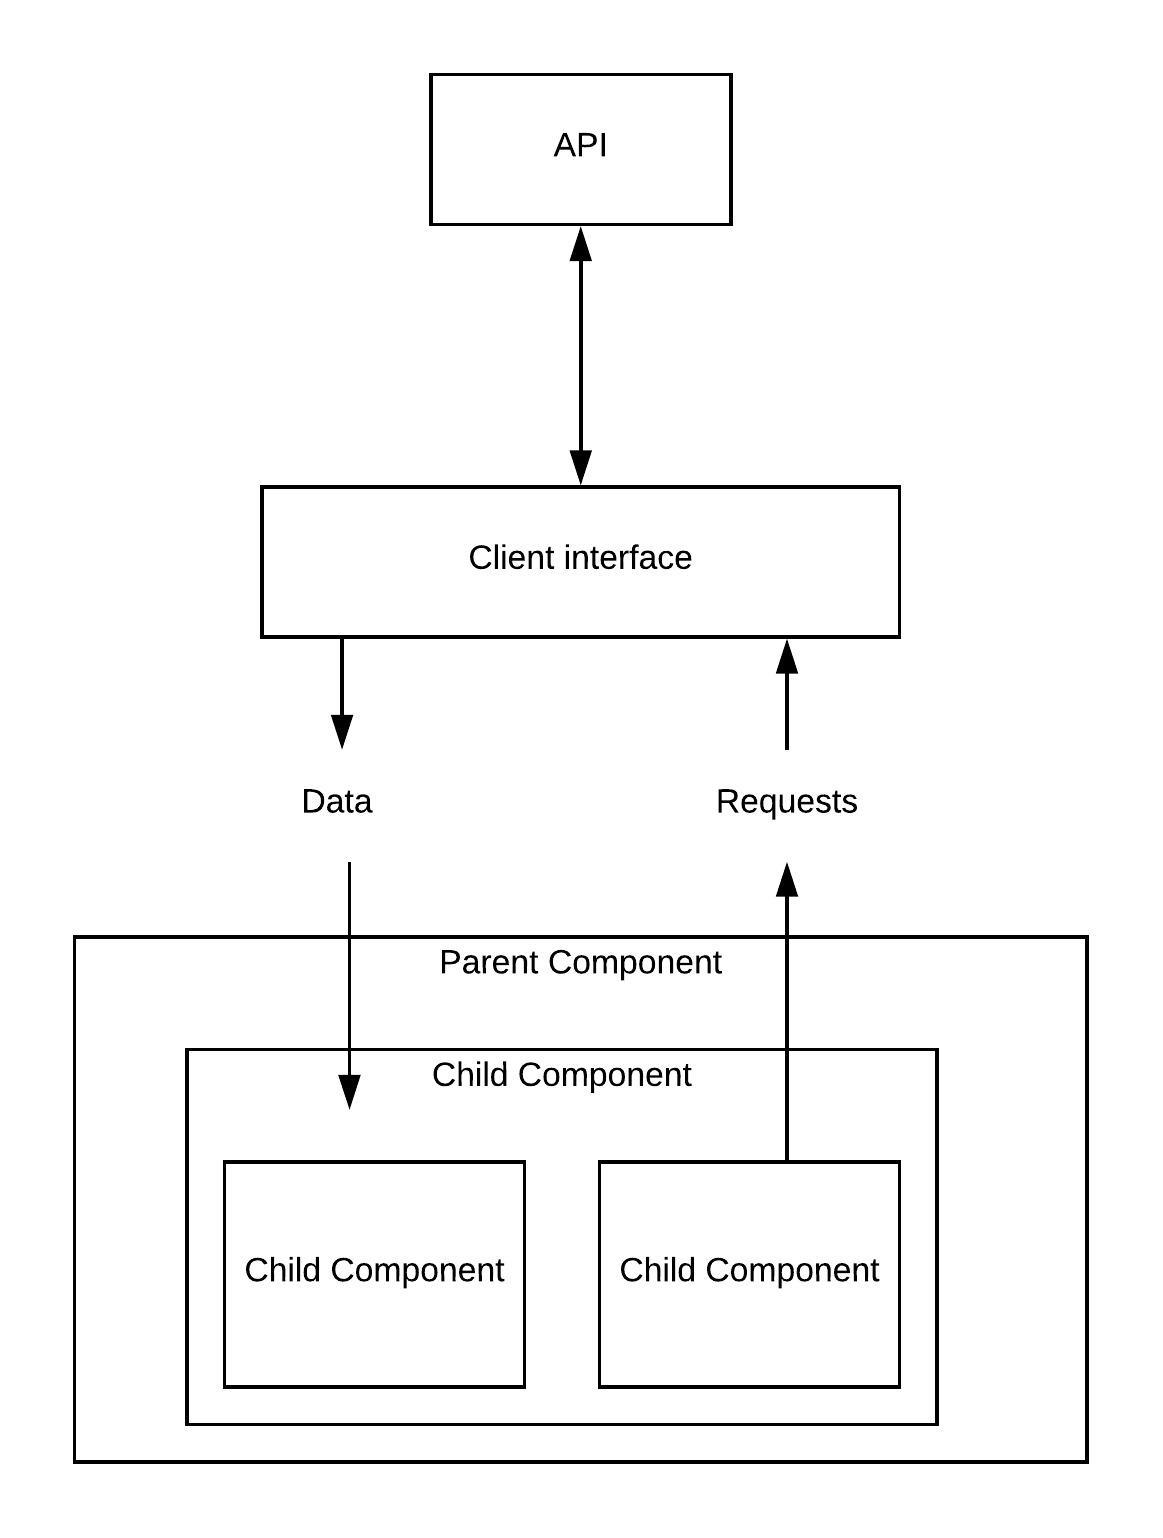
\includegraphics[origin=c]{./diagrams/front-end-diagram.jpeg}
        \label{front-end}
    \end{figure}
    
    \subsubsection{Testing}
    Testing the front-end app is a relatively new trend in web development and it has been made very easy with libraries like Jest, written by Facebook. Jest can send mocked data through the app and take “snapshots” of the rendered components. When front-end code changes, the tests will fail in an expected way, then the developer can confirm the changes made with the new snapshot. When tests fail unexpectedly, this is still good, because Jest is catching some unwanted side effects that need to be addressed.

    In addition to snapshot testing, functional testing is available to test any visual dynamic behavior. For example, if there is a drop-down menu, a good unit test for it would be that it opens and closed accordingly when clicked. Although it is tedious test for a human to do, Jest allows us to automate it, so the team benefits from additional unit testing without spending the extra time on it.
    
    \subsection{API}
    \subsubsection{Typescript Conversion}
    We will convert the back-end code from pure Javascript to Typescript because it is a super-set of JavaScript and therefore backwards compatible. The process of converting will be fairly quick. This will primarily involve defining types and adding those types to the appropriate variable declarations and functions. Types provide better readability for those coming to the project as well as ensure robustness in code as it is written. The following is an example of a JavaScript function compared with its TypeScript counterpart.\\
    JavaScript:
    \begin{minted}[
        xleftmargin=18pt,
        linenos,
        autogobble,
        breaklines,
    ]{javascript}
        buildUpdateString (keys, values) {
            keys = keys.split(',')
            let query = ``
            let idx = 1
            for (var i in keys) {
              let key = keys[i]
              query += `${key} = \$${idx}, `
              idx++
            }
            query = query.substring(0, query.length - 2)
            return {
              query,
              idx
            }
          }
    \end{minted}
    TypeScript:
    \begin{minted}[
        xleftmargin=18pt,
        linenos,
        autogobble,
        breaklines,
    ]{javascript}
        buildUpdateString (keys: string, values: string): IUpdateString {
            let key_list:string[] = keys.split(',')
            let query: string = ``
            let idx: number = 1
            for (let key in key_list) {
              query += `${key} = \$${idx}, `
              idx++
            }
            query = query.substring(0, query.length - 2)
            return {
              query,
              idx
            }
          }
        \end{minted}
        In the situation above, the type \verb:IUpdateString: would also have to be defined, but it would also be used in other functions that return the same type of value.
    \subsubsection{New Functionality}
        Due to updates being made in the database and the front-end, we will have to similarly update the back-end so that data can be passed between the two without issue. This functionality will mirror much of the logic already implemented and will be written directly in TypeScript. It will have query functions to update and retrieve data from new database tables as well as REST protocol functions to update the user interface and receive changes.
    \subsubsection{Testing}
        We will write testing for the back-end using Jest. This requires that we create a mock database for these functions to hit, running different types of valid and invalid data through them. We will make sure that all types of valid data presents us with correct results and that invalid data is handled properly such that it does not crash the application. This will improve the consistency of the application by showing that at least all of the known cases can be handled. It will also help with future development because team members can check that, when they make changes, the application still behaves in the expected fashion.
        
    \subsection{Dev-Ops}
        \subsubsection{Container}
            Docker will be used as our container for each instance of our application. The Docker containers will allow us to compartmentalize instances, giving us the ability to test and deploy multiple in a very short amount of time. It will help considerably if the website gets heavy traffic, preventing it from being bogged down with many requests. This will be the first part of the Dev-Ops tasks that will need to be setup as this is the most basic building block of our web application.
             
            These containers will be set up on virtual machines hosted on Amazon Web Services, which are then load balanced. Once the Docker containers are fully functional and tested, we can then move on to setting up the load balancer.
            
        \subsubsection{Cloud Storage and Load Balancing}
            We will handle load balancing and storage through Amazon Web Services.
            The containers will need to live somewhere, and so will the data they collect. Using Amazon Web Services, we will be able to spin up our containers on the cloud, and use Amazon's Elastic Load Balancing tools to direct traffic. 
            With multiple containers getting an even amount of traffic through the load balancer, we should not have a problem with constant up-time and little to no downtime on our site. 
            
            Amazon Web Services will also be where we can store our database of information on tanks, batches, history, etc. The information will be available to all of the Docker containers, and will be accessed through the client interface to the API. See \textbf{section 3.2.2} for more information on sending and receiving information to the API.
    
            Once we have load balanced Docker containers, we can test traffic throughput and make sure our load balancer can handle enough if not more traffic than we anticipate. Once we move past the load balanced container and have it all set up correctly, we can host it on Amazon Web Service's EC2.  
        
        \subsubsection{Web Hosting}
            As of now, the website is hosted on a previous student's Oregon State ENGR server. Our goal is to take the site down, and set it up on a more professional, business-grade environment.
            Similarly to our Cloud Storage and Load Balancing, we will be using Amazon's EC2 hosting option to distribute our website. Amazon's EC2 gives us a lot of easy options when working in unison with their elastic load balancer. EC2 hosting will take requests and forward them to our load balancer, which will be the elastic load balancer. From there, the load balancer will decide on which Docker Container the user should go to, based on traffic.
            
            Web hosting can be tested easily, using Amazon Web Services built-in diagnostic tool, and also by checking the container id's when going through each instance. It can be usability tested also by checking and seeing if the sites load properly. 
            
        \begin{figure}[h]
            \centering
            \label{fig:my_label}
            \caption{Left side represents our Web Hosting URL. It then cascades down to the Load Balancer and then to each instance and container}
            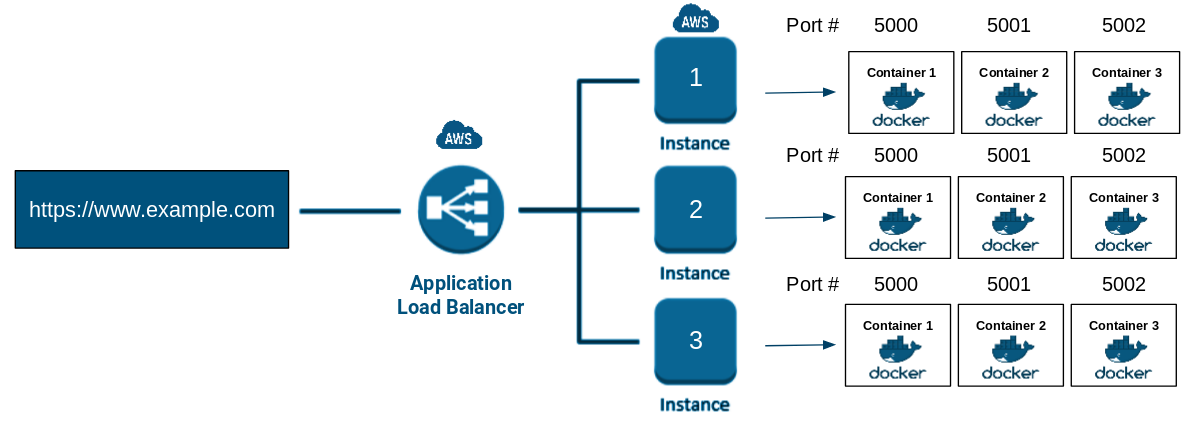
\includegraphics[width=6.5in]{img/load-balance-architecture.png}
        \end{figure}          
    
\section{Appendix}
    \subsection{Desktop Design}
    \begin{figure}[H]
        \centering
        \caption{The Login page for desktop}
        \fbox{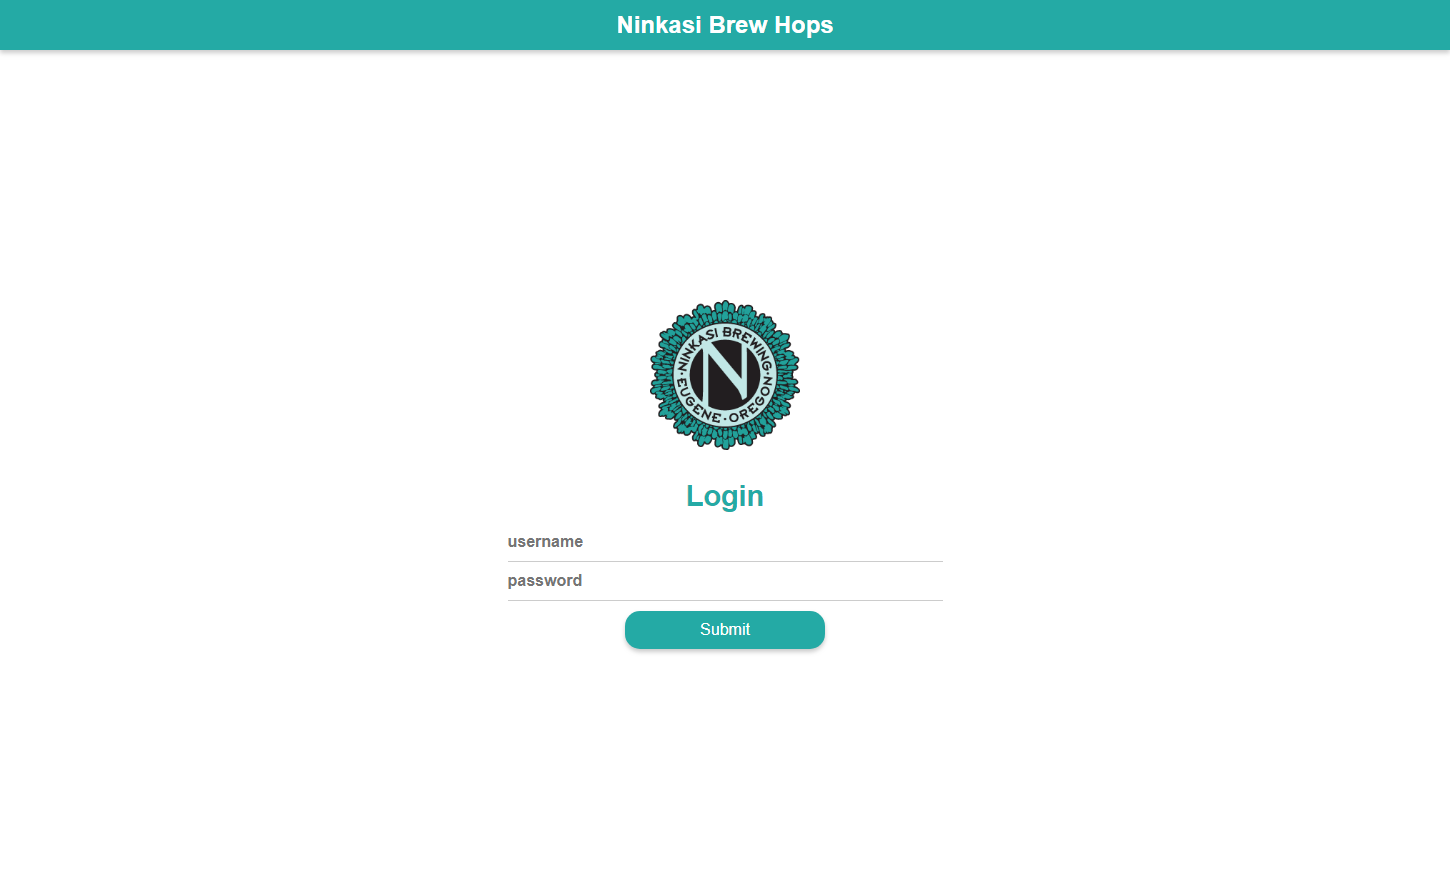
\includegraphics[origin=c,width=6in,keepaspectratio]{./img/login-page.png}}
        \label{login-page}
    \end{figure}
    \begin{figure}[H]
        \centering
        \caption{The desktop homepage}
        \fbox{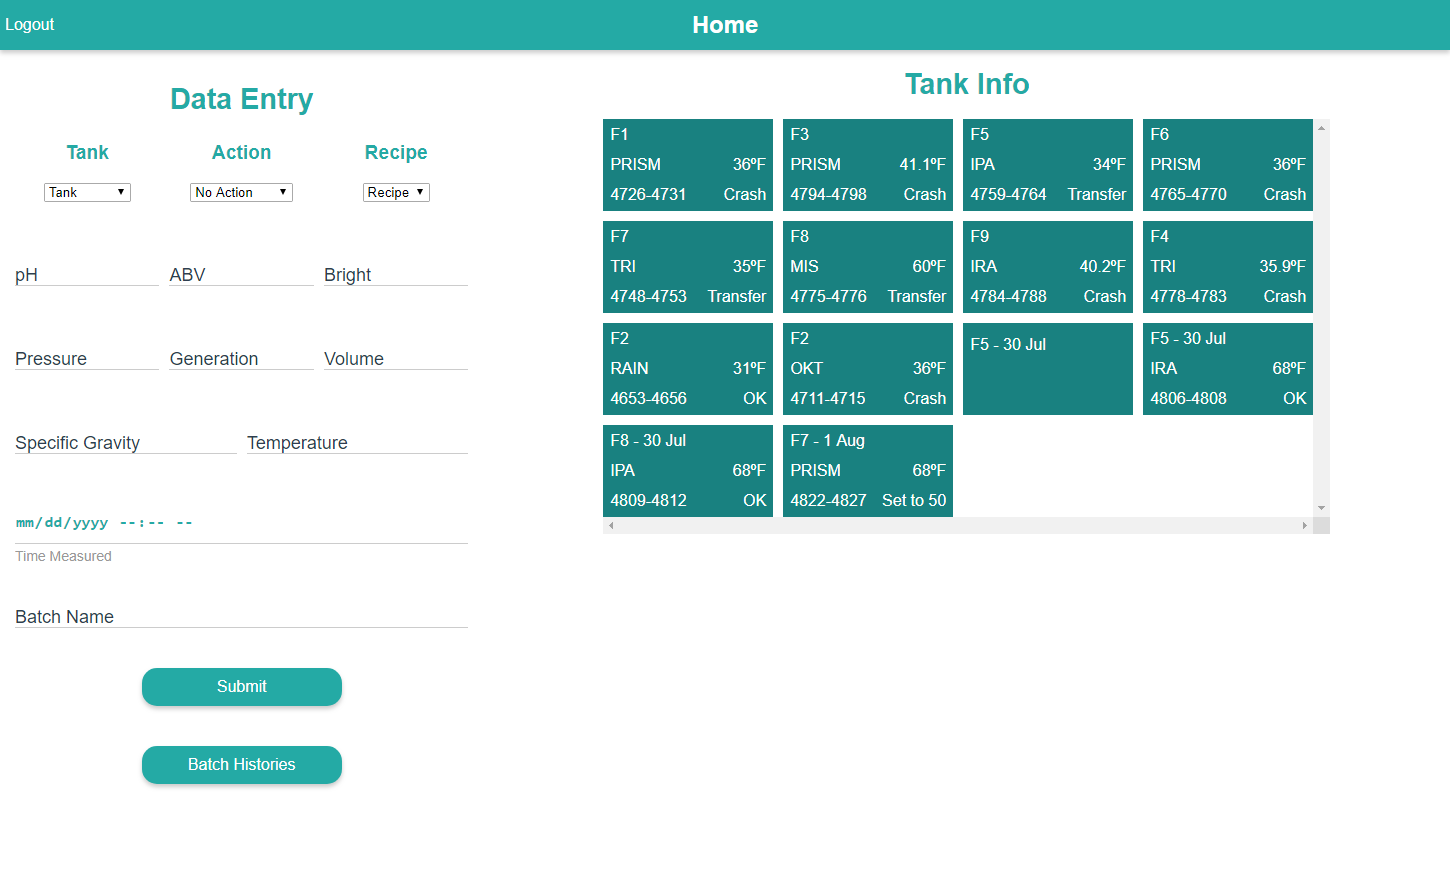
\includegraphics[origin=c,width=6in,keepaspectratio]{./img/home-page.png}}
        \label{home-page}
    \end{figure}
    \begin{figure}[H]
        \centering
        \caption{The tank information page}
        \fbox{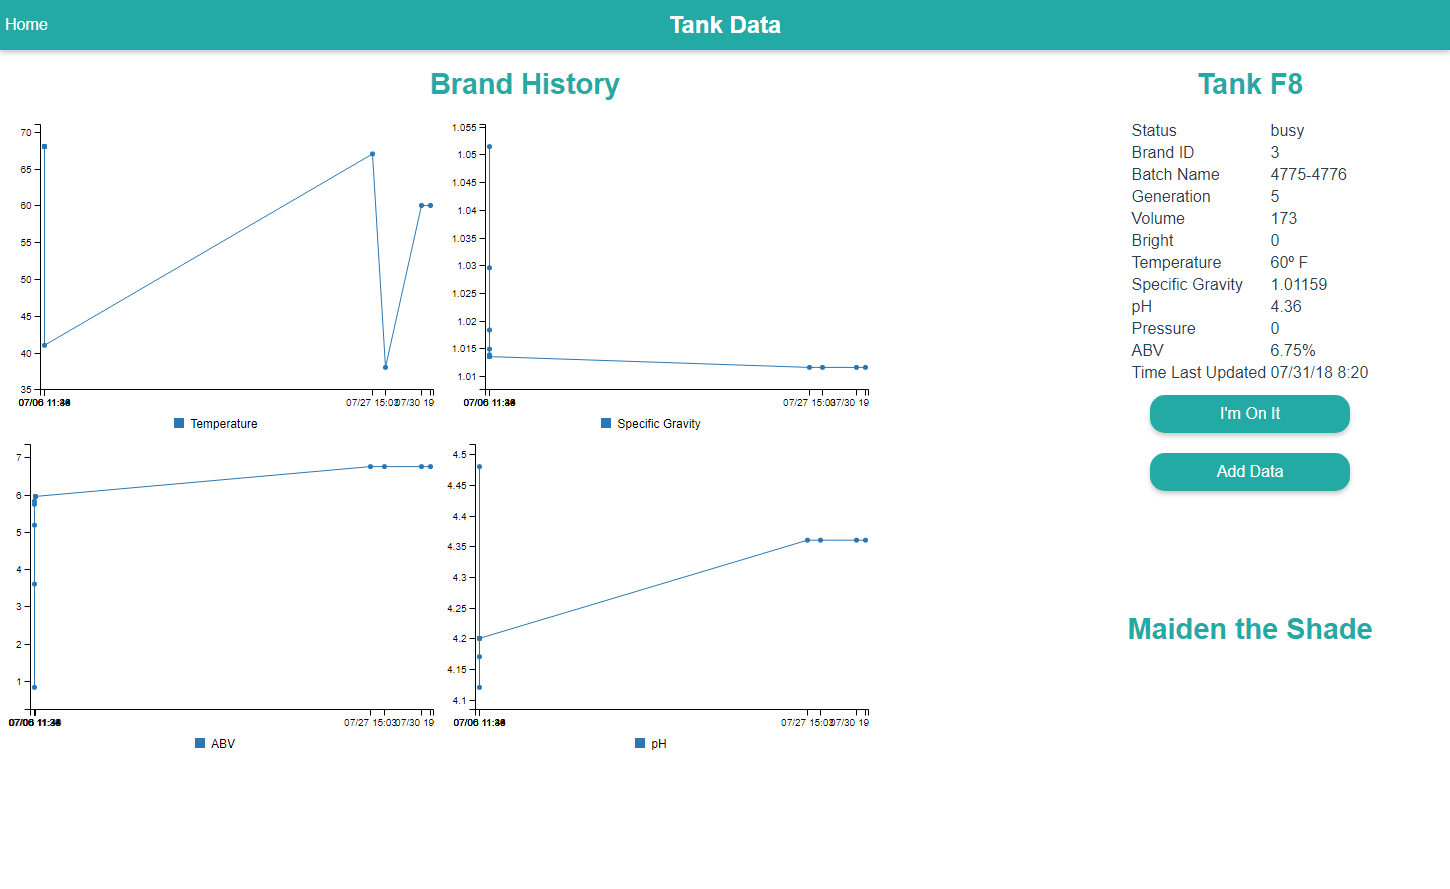
\includegraphics[origin=c,width=6in,keepaspectratio]{./img/tank-page.png}}
        \label{tank-page}
    \end{figure}
    \begin{figure}[H]
        \centering
        \caption{The data entry page}
        \fbox{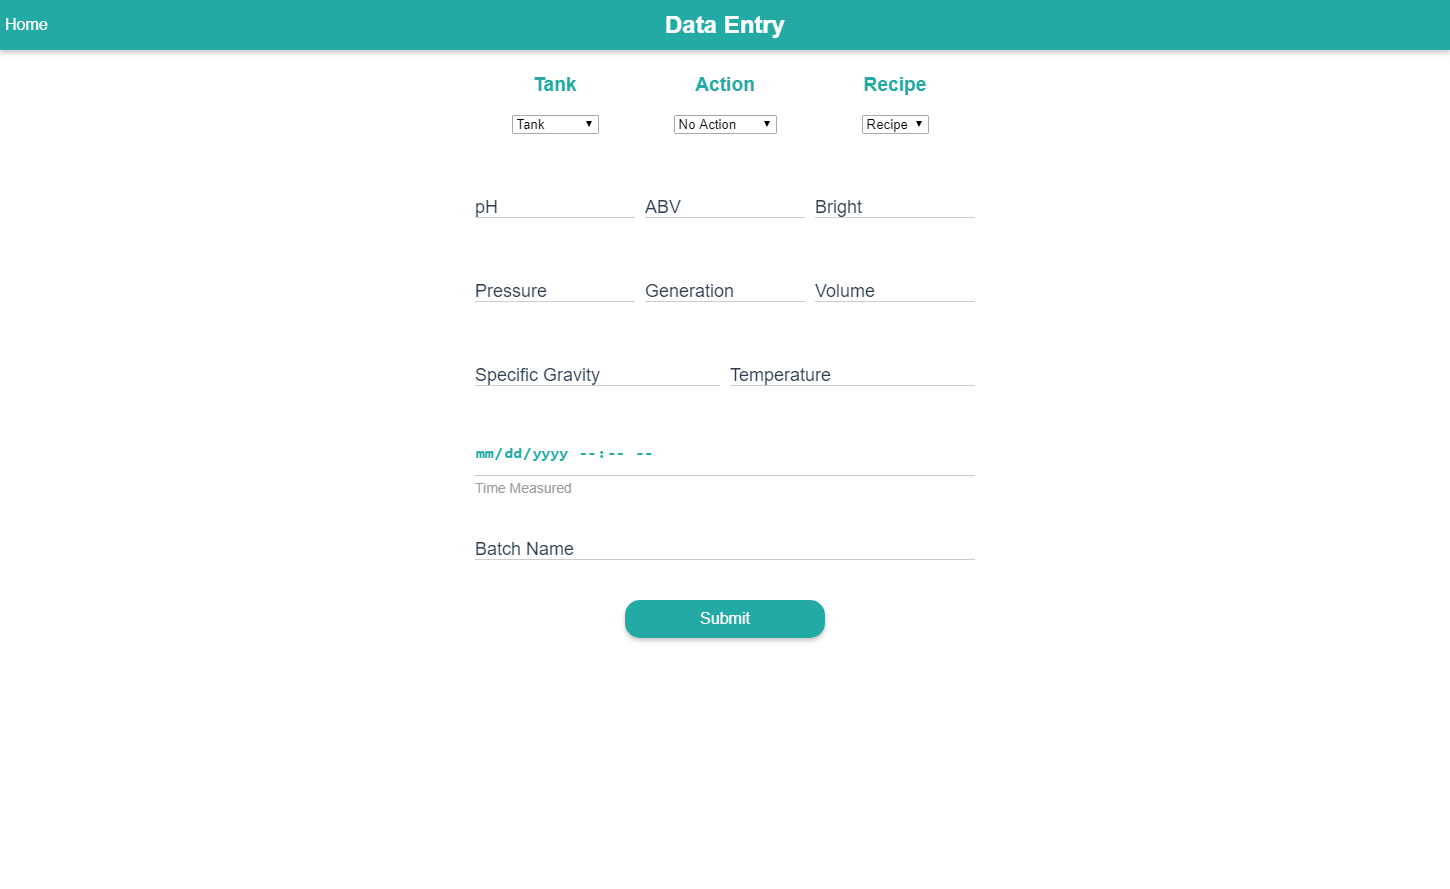
\includegraphics[origin=c,width=6in,keepaspectratio]{./img/data-entry.png}}
        \label{data-page}
    \end{figure}
    
    \subsection{Mobile Design}
    
    \begin{figure}[H]
        \begin{multicols}{3}
            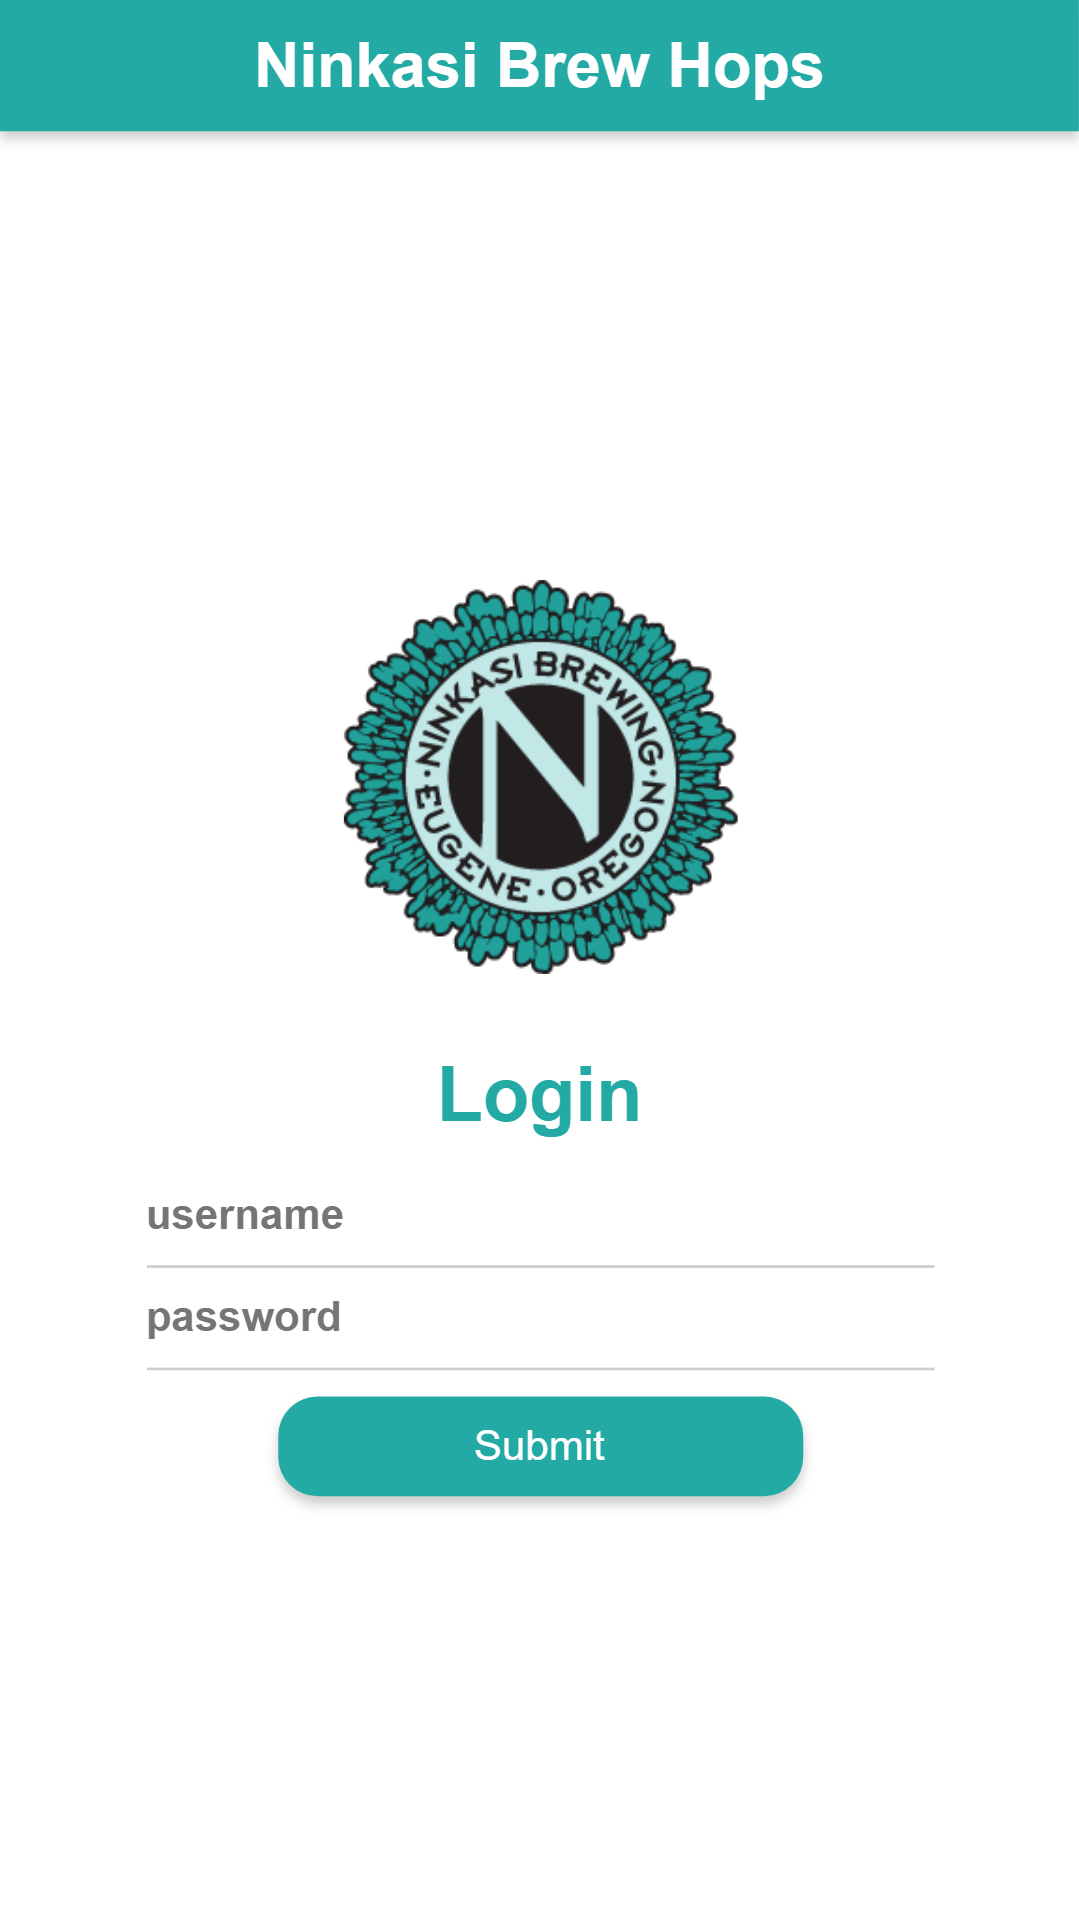
\includegraphics[width=\linewidth]{./img/mobile-login-page.png}
            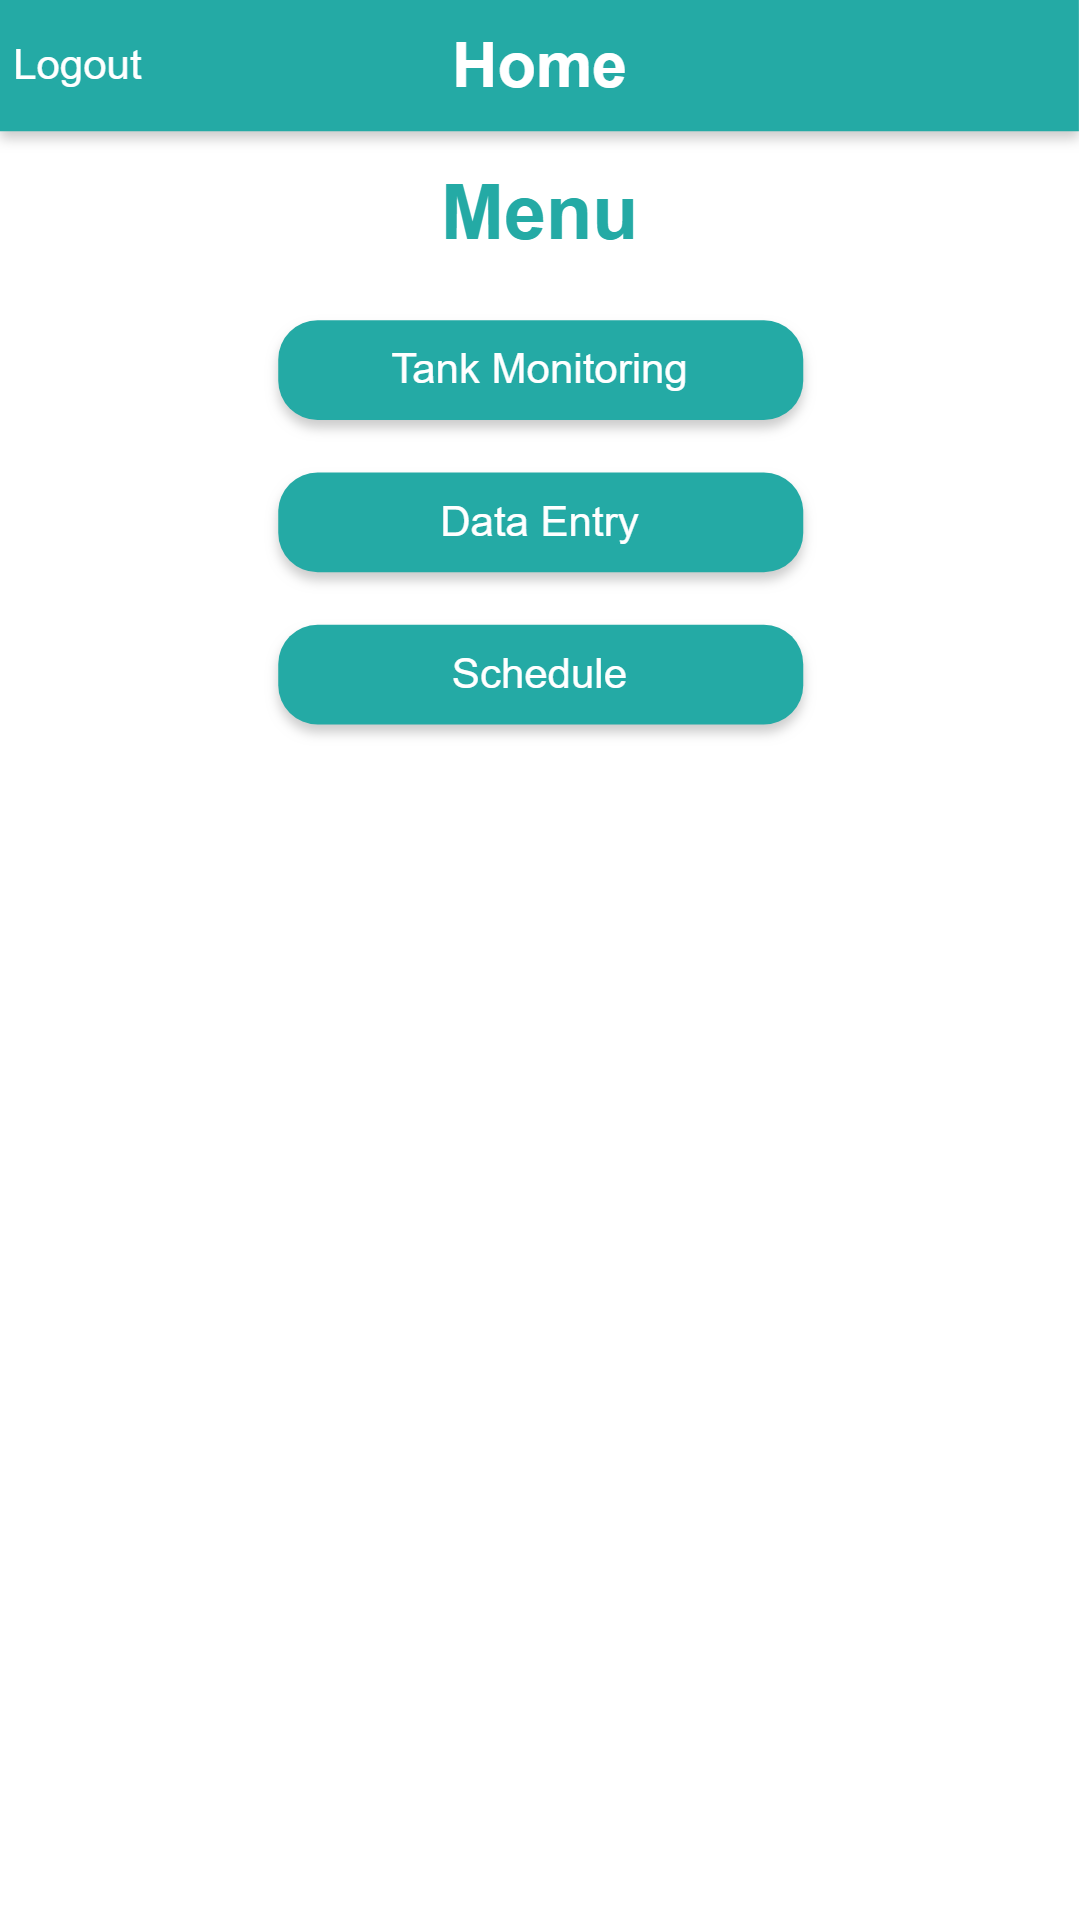
\includegraphics[width=\linewidth]{./img/mobile-home-page.png}
            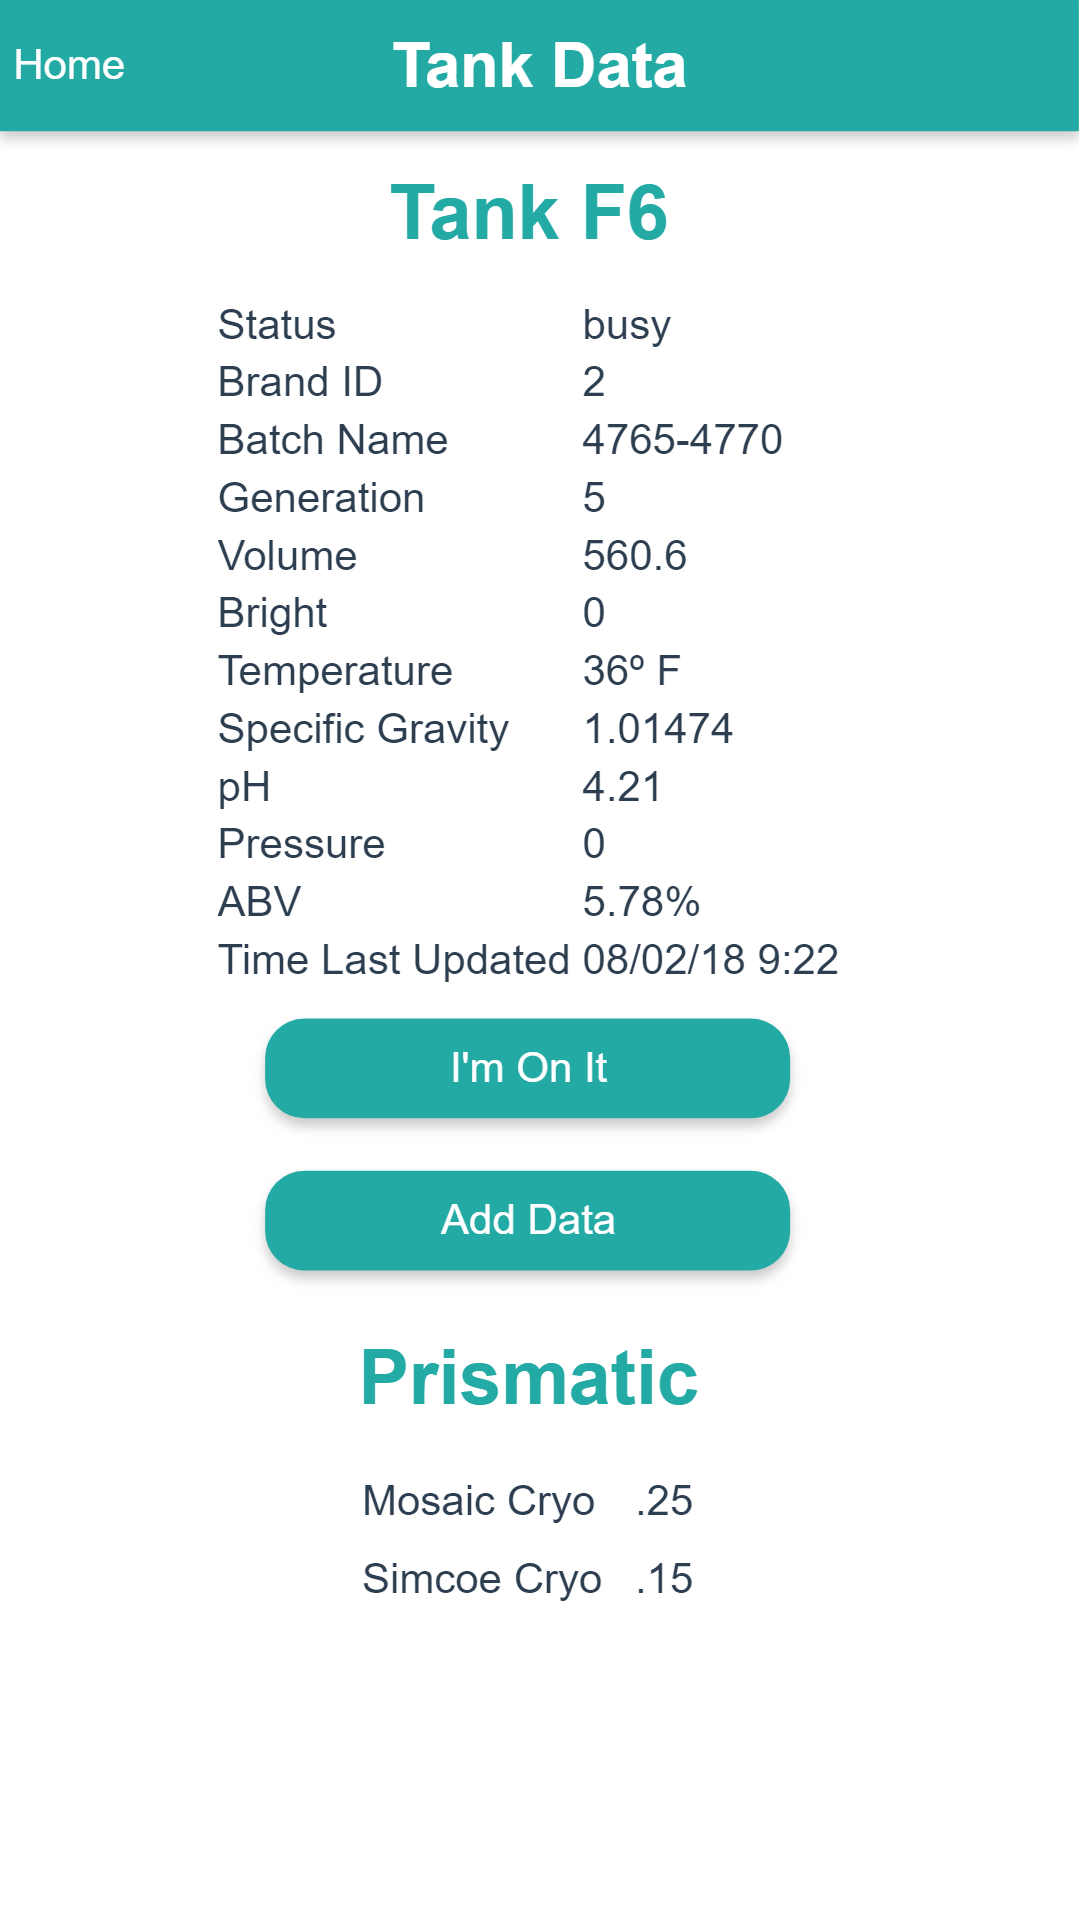
\includegraphics[width=\linewidth]{./img/mobile-tank-page.png}
        \end{multicols}
        \caption{Mobile layouts from left to right: login page, home page, tank page}
    \end{figure}
    
    \pagebreak
    
    \begin{figure}[H]
        \caption{Mobile layouts from left to right: admin page, data entry, tank info}
        \begin{multicols}{3}
            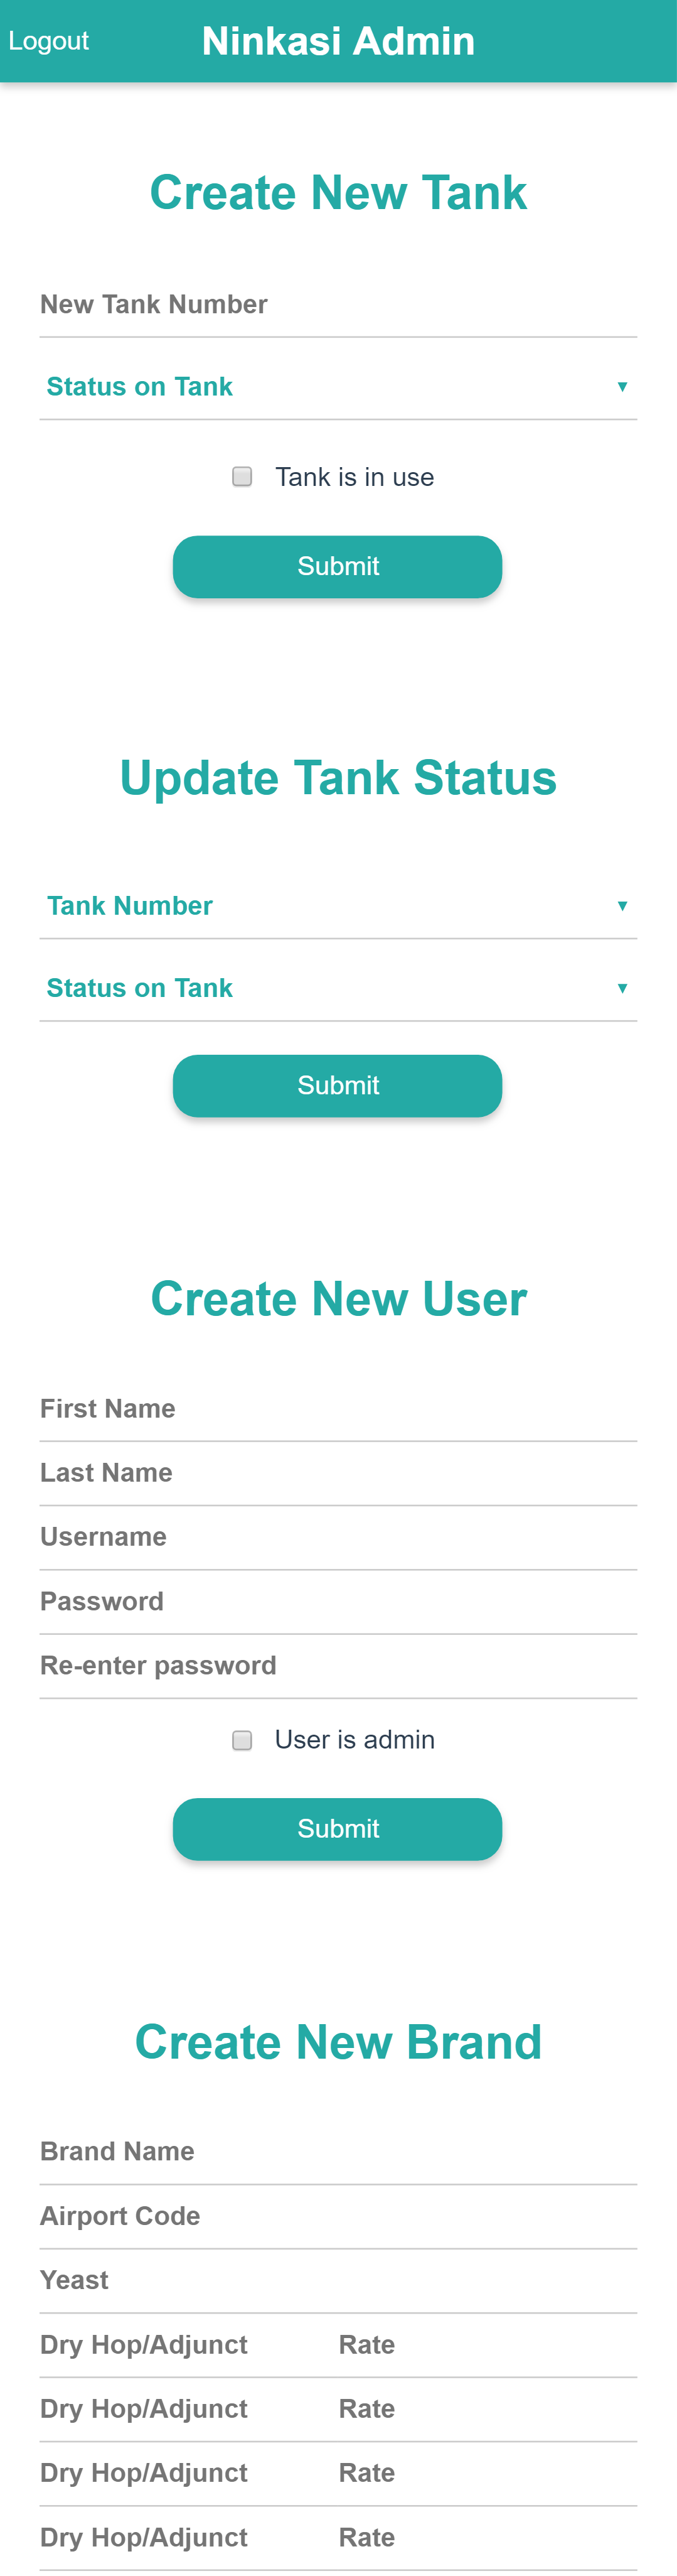
\includegraphics[width=\linewidth]{./img/mobile-admin-page.png}\par
            \adjustbox{trim=0cm 7cm 0cm 0cm,clip}{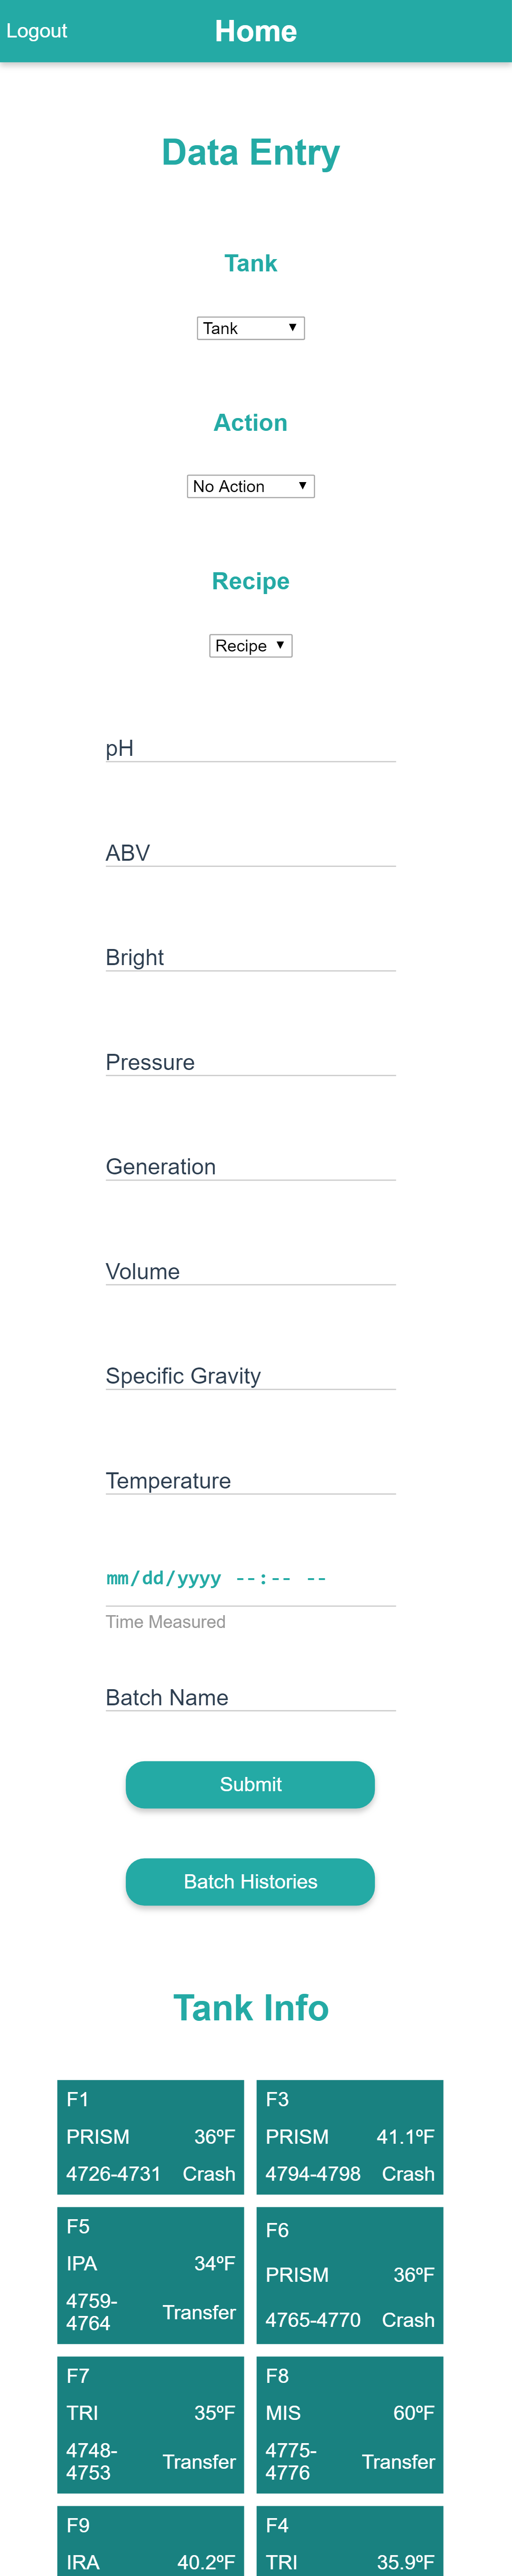
\includegraphics[width=\linewidth]{./img/mobile-data-entry.png}}\par
            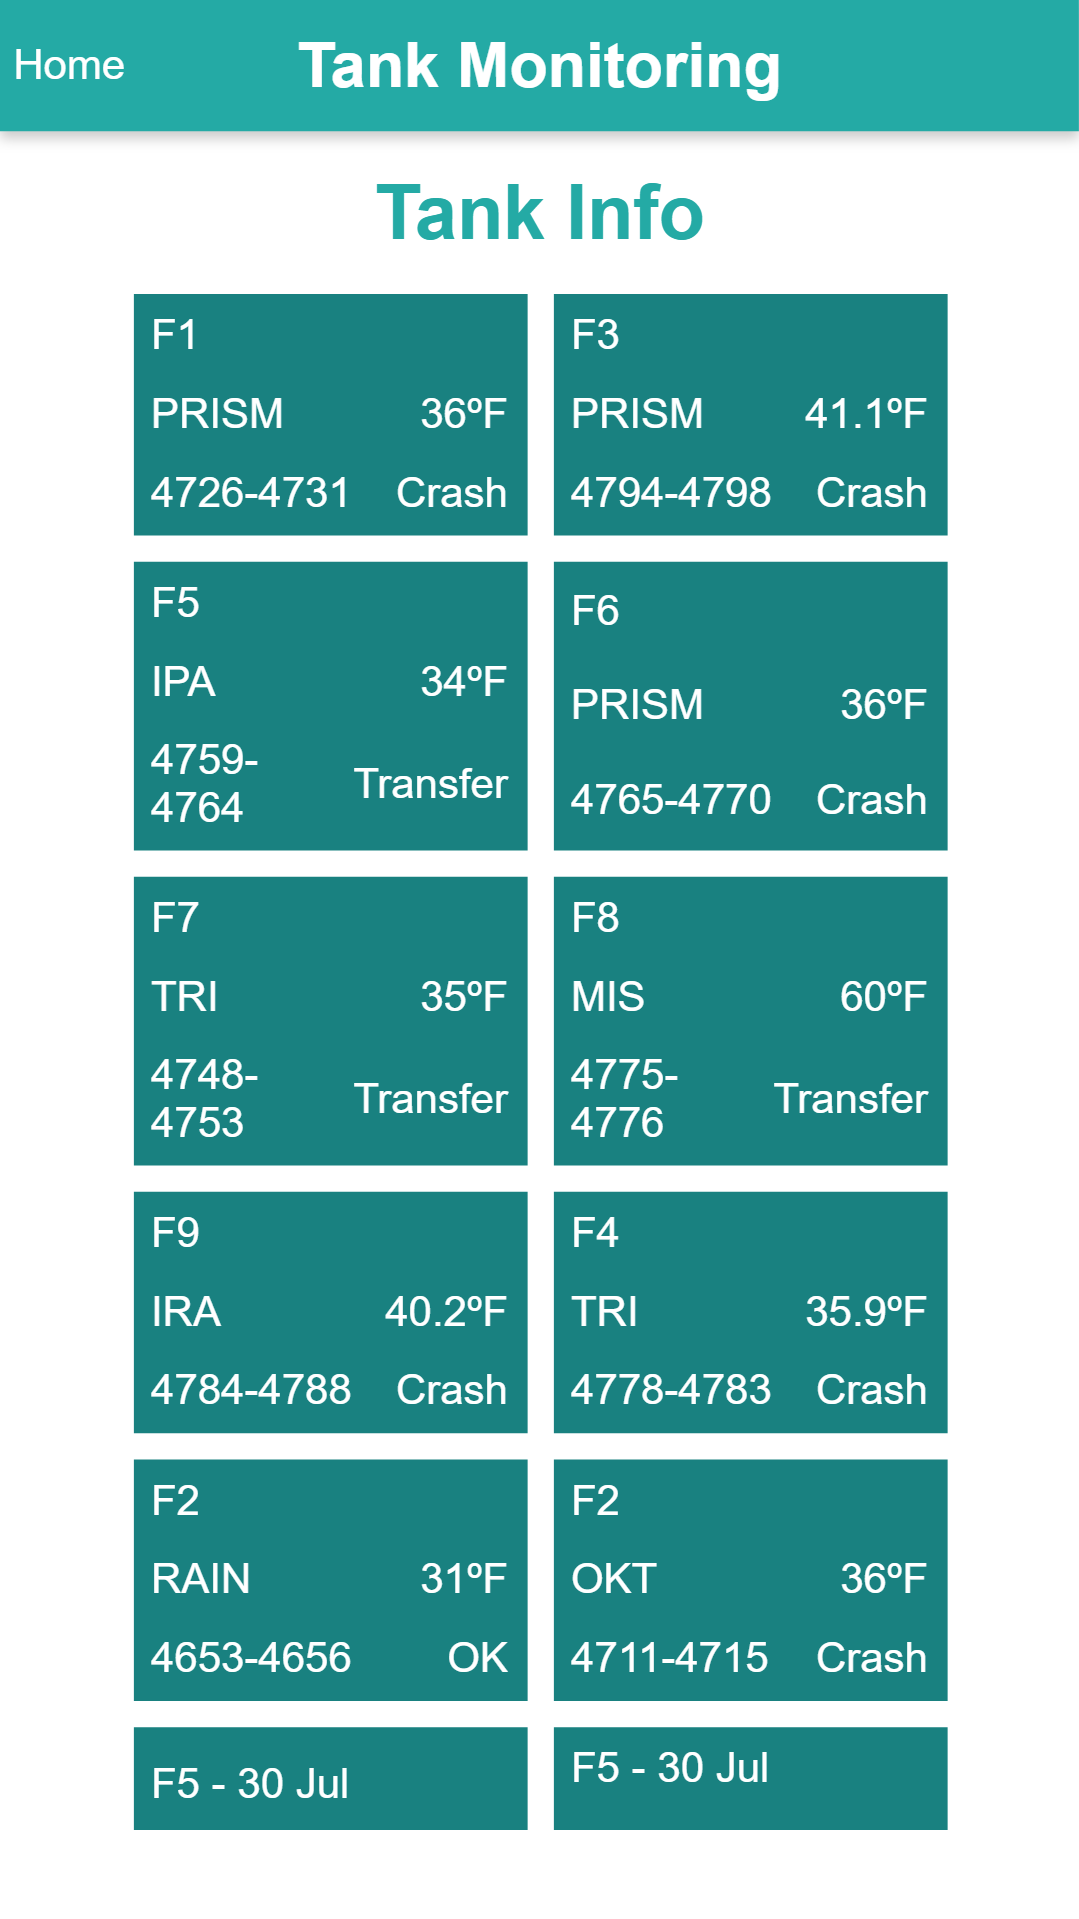
\includegraphics[width=\linewidth]{./img/mobile-tank-info-page.png}\par
        \end{multicols}
            
    \end{figure}
}

\newpage
\section{Tech Reviews}

\subsection{Brennan Douglas}
{
    \let\section\subsubsection
    \let\subsection\subsubsubsection
    \let\subsubsection\subsubsubsubsection
    
\section{Introduction}

The application being built is for Ninkasi.  Currently, Ninkasi keeps all of their data in an excel spreadsheet; this gets passed around among different people who enter different bits of data from paper forms.  This is a very ineffective way to store such valuable information.  It restricts who can see the data, as well as who knows if they are looking at current data.  This method is also heavily prone to error as entries can be easily changed by accident without any knowledge of this occurring.  There is no history feature to keep track of edits, neither their changes or authors.  A solution to solve this has already begun in the form of a web app, however it was left in an unfinished state.  All data needs to be manually input through the forms of the website.  This creates a blocking point for inputting historical data as it is in the tens of thousands of data points.  The core functionality of the application already exists, but it needs to be re-factored to become usable.  Additionally, extra quality of life features need to be added and the application needs to be polished for a production environment.

The team, BrewHops, has decided that all of our teammates will be familiar with the entire application, we are all full-stack developers.  However, we have split the technologies for the propose of the tech reviews.  This tech review focuses on the back-end aspects of the application.  The sections will build off of the previous, based on the conclusion reached for the former technology.  This helps limit the scope of the technologies to choose from, otherwise the number of technologies would be overwhelming.  First, the format of data in the database in needs to be determined.  This involves discussions of how structured it needs to be, the convince of development, and the support for the style.  From there, databases that support that type of format will be researched and compared to make the best decision.  Finally, the best archival solution will be determined for Ninkasi given the recommended database.

\section{Data Model}

    \subsection{Introduction}
    
    The way that data is modeled is very important to an application.  It defines how the different query behavior will be implemented and which aspects of the application will be easier or harder to implment.  There are two main categories of data modeling that are revelvant to look at: SQL, and NoSQL.  SQL has been the standard for a long time, however with issues of scale at the much larger tech companies NoSQL formats have been created \cite{sqlizer}.
    
    \subsection{NoSQL}
    
        \subsubsection{Summary}
        
        There are many different types of NoSQL data models.  This is because NoSQL is equivalent to the phrase non-relational data bases, "not SQL".  NoSQL models are primary designed around being very fast at scale for their particular use case.  The various different types include: key-value pairs, document, and graph \cite{amazon_nosql}.  The most common type is the document class of NoSQL models.  In these, entries are just JSON objects, meaning they can be easily spread out across multiple different machines to horizontally scale the database.  Out of all the different forms of the NoSQL data models this class, the document style, would be the most appropriate for our use case.  This is because we have a few main entities that could be represented as separate documents.  Each of these documents would then contain very piece of information they need, rather than being normalized across many different tables.
        
        \subsubsection{Pros}
        
        \begin{itemize}
            \item Horizontally scalable
            \item Quick development
            \item Simple queries
            \item No dedicated database server required (depending on database engine)
        \end{itemize}
        
        \subsubsection{Cons}
        
        \begin{itemize}
            \item Deep models
            \item Data replication
            \item Large query responses
        \end{itemize}
    
    \subsection{SQL}
    
        \subsubsection{Summary}
        
        As mentioned previously SQL is the oldest of the database models.  It has been around for over 40 years \cite{sqlizer}.  It allows the data to be normalized across many different tables reducing data replication.  It also has far more support than other technologies due to its ubiquity.  It would also allow for more precise query calls to be made retrieving only the information that is required from the database.  This last point is key as our application is targeting mobile devices where networking are a limiting factor.
        
        \subsubsection{Pros}
        \begin{itemize}
            \item No data replication
            \item Precise queries
            \item Ubiquitous support
            \item Data integreity
        \end{itemize}
        
        \subsubsection{Cons}
        \begin{itemize}
            \item Structured (sometimes overly so)
            \item Dedicated database server required
            \item Slow development
        \end{itemize}
    
    \subsection{Conclusion}

    In conclusion, simply due to the support available, SQL is the best choice.  Ninkasi should have the highest number of options available to them when it comes to choosing their environment, this SQL provides.  A large factor is also the data integrity.  These SQL engines have been being used for decades, they are well and thoroughly tested.  Ninkasi can be assured that their data will not be lost or corrupted.

\section{Databases}

    \subsection{Introduction}
    
    Now that the data model has been chosen, different database engines can be looked into.  There are a few different options that are standard when wanting to work with SQL: PostgreSQL, MySQL, SQL Server.  This vary very little in their syntax and functions as they have all been copying each other for a long time.  There are categories which they differ in, most notably if they are free or not.  This is important for small projects as it is hard to justify spending money on something that has very few benefits over another.  Especially when it is well supported and free to use.
    
    \subsection{PostgreSQL}
    
        \subsubsection{Summary}
        
        PostgreSQL is a powerful open source SQL database engine \cite{postgresql}.  It has the same query syntax as the other open source SQL database engines out there.  However, it also has strong support for some very NoSQL like features.  This allows the advantages of SQL and NoSQL to be combined from the model viewpoint.  Though, it cannot capture the scalability advantages of the different NoSQL systems as it is NoSQL within a SQL database.
        
        \subsubsection{Pros}
        \begin{itemize}
            \item Open source
            \item Free
            \item NoSQL features
            \item Runs on almost anything \cite{db_comparison}
        \end{itemize}
        
        \subsubsection{Cons}
        \begin{itemize}
            \item Not the most popular
            \item Not the same level of support as MySQL
        \end{itemize}
    
    \subsection{MySQL}
    
        \subsubsection{Summary}
        
        MySQL is another powerful open source database management system.  It is more popular that PostgreSQL, yet actually has fewer features \cite{db_comparison}.  MySQL stands in a funny spot within the open source line up, it has been acquired by Oracle \cite{mysql}.  This makes some in the community unsure of its future longevity as a free and open piece of software.  This is due to it directly competing with one of Oracle's main paid offerings.  However, MySQL is often the go to open source SQL database management system, especially for small projects.
        
        \subsubsection{Pros}
        \begin{itemize}
            \item Popular
            \item Highest level of third-party support
            \item Open source
            \item Free
        \end{itemize}
        
        \subsubsection{Cons}
        \begin{itemize}
            \item Not as many features as PostgreSQL
            \item Rudimentary NoSQL support
        \end{itemize}
        
    \subsection{SQL Server}
    
        \subsubsection{Summary}
        
        SQL Server is Microsoft's SQL database management system.  It is a commercial grade application, and comes with the price to prove it.  It does provide more advanced functionality than either MySQL or PostgreSQL, however these are features that are not needed by the application \cite{sql_server}.  There is no strong point for a discussion with Ninkasi to even be approached about buying a license for SQL Server.  Also, MySQL's and PostgreSQL's syntax is identical in almost all cases, this is not the true for SQL Server as it diverges in some subtle locations.
        
        \subsubsection{Pros}
        \begin{itemize}
            \item Advanced functions
            \item Best performance
        \end{itemize}
        
        \subsubsection{Cons}
        \begin{itemize}
            \item Cost
            \item Commercial
            \item Different syntax
        \end{itemize}
    
    \subsection{Conclusion}

    In conclusion, PostgreSQL provides the application with the most flexibility and support.  It will can on anything that Ninkasi could ever want, and has a large community of support and third-party interfaces ready to be used.  SQL Server is too much for this project as it does not have the complexity or amount of data where its features and performance benefit over MySQL or PostgreSQL.  It is also important to keep the cost of the system to a minimum for Ninkasi as this is replacing a currently free process.

\section{Archival Process}

    \subsection{Introduction}
    
    It is important to make sure that Ninkasi never loses any of the data they store in the application.  So, a database archival process will be implmented.  This allows them to restore or role back their data to a previous time if they ever need to.  "Database archiving is the process of intelligently moving historical data from production environments to an archive environment, freeing up IT storage space and other resources" \cite{ibm_archiving}.  As we have chosen PostrgreSQL as our database management system only archival solutions for that platform will be focused on.  Key factors that are under consideration for an archival process are: data integrity, consistent archiving, and minimized storage space.
    
    \subsection{PostgreSQL WAL}
    
        \subsubsection{Summary}
        
        PostgreSQL's write ahead log, WAL, is the log file where it stores every operation done to the database along with the time at which it happened \cite{postgresql_wal}.  This file was originally designed, and still used for, crash recovery where some of the command had yet to be completed at time of failure.  PostgreSQL simply rolls back to the last safe state and then replays the executions from the WAL.  The WAL is simply just a file that is stored on the file system, this means that it can be copied to a safe archival location.  If this is done on a regular process the entire database can be reconstructed from these files.  It provides another feature hidden in its time stamps on the queries, it allows for point-in-time recovery \cite{postgresql_wal}.  This means the database can be reconstructed up until any point in time the user would like, with no extra storage cost associated.
        
        \subsubsection{Pros}
        \begin{itemize}
            \item Continuous archiving
            \item Point in time archiving
            \item First-party support
            \item Assured data integrity
        \end{itemize}
        
        \subsubsection{Cons}
        \begin{itemize}
            \item Must manually create scripts to copy the files
            \item Special configuration setting must be turned on
            \item Data isn't available until a database is built from the files
        \end{itemize}
    
    \subsection{Manual Archival Scripts}
    
        \subsubsection{Summary}
        
        Manual archival scripts refers to the process of manually writing archival queries that transfer specific data to the archive location.  This would require a lot of manual work to figure out what needs to be saved, the difference between the current database and the archive database, and the expense cost of needing to run this while the database is trying to function for the application.  This is inherently error prone as it is only supported by the developers of the application.  Therefore, it would need to be updated with any updates to the database.  This provides another point of failure.
        
        \subsubsection{Pros}
        \begin{itemize}
            \item Only copies and stores data that cannot be replaced
            \item Data will be stored in another database that can be queried
        \end{itemize}
        
        \subsubsection{Cons}
        \begin{itemize}
            \item Higher potential for loss of data due to human error
            \item Manually intensive
            \item Not maintainable
        \end{itemize}
    
    \subsection{Conclusion}
    
    The choice is pretty simple given that there are not many options, PostgreSQL's WAL archival process.  This provides the most features right out of the box and will require the least manual work to getting moving.  It also has the promise of strong data integrity which is a key aspect of archiving.


}

\subsection{Dan Van Horn}
{
    \let\section\subsubsection
    \let\subsection\subsubsubsection
    \let\subsubsection\subsubsubsubsection
    \section{Introduction}
We are continuing development on an existing solution from a previous capstone group. It includes a small set of applications designed to manage brewing data automatically, allow for manual user editing, and generate graphic visualizations. This system will manage brewing data quickly, efficiently, and correctly as it will reduce the possibility for human error. The applications will be hosted on a cloud provider and be both desktop and mobile compatible. Each developer role in the project is to be adaptable and familiar with the entire technology stack we are implementing.
\section{Front End}
The state of web application development has moved past serving static html pages, style sheets, and JavaScript. With the demand for dynamic content and more user features, there has been significant advancement in front-end frameworks that can be developed in a more readable language and allows for the creation of dynamic web applications. These frameworks use a process called transpilation to transform the source code into a bundled application that can be executed by all modern browsers. This is one of the criteria for a Progressive Web Application which would be a benefit for Ninkasi because they plan to use this application cross platform with possibly unreliable internet connection. From a project perspective, the use of these frameworks has the benefit of quicker development, superior code modularity, and testability. The existing front-end application is written in Vue.js, one of the frameworks we review for its practical applicability among other potential candidates.
    \subsection{React}
    React is a front-end framework developed by Facebook and one of the most popular libraries used in industry today. It uses a quicker virtual DOM instead of the traditional DOM which increases performance and can be rendered on clients and on servers. It encourages the developer to utilize reusable UI components that are dynamic. Data flows unidirectionally through these components, which makes the application easier to reason about and avoids unintended side effects during runtime. 
    
    The front-end logic can be written in JavaScript and use a templating language called JSX to build the app views. There is a slight learning curve to the React style of programming, but many engineers clearly prefer this technology as it is the top-ranking technology in terms of engineers that have used it before and would use it again \cite{stateofjs2017}.

    \subsection{Vue}
    Vue is a similar technology to React in that it is primarily concerned with the front-end aspect of the application. It was developed and is maintained by an international community of software engineers. Like React it also utilizes a virtual DOM, promotes the use of composable reusable components and allows for other libraries to be integrated with ease. One main difference is that in Vue, the use of the JSX templating language is unnecessary and html can be used instead. JSX is an option with Vue as a plugin, so in some ways that is a major advantage. 
    
    There are no major performance advantages between the two however, so the real decision come down to the preference of the coding syntax. As huge benefit to Vue is the concept of single file components. These components contain the template, logic and style for a section of the application \cite{vue}. This simple organization is a huge advantage and is no doubt one of the reasons why the previous group that worked on this project chose it as their front-end framework. Although it is not as widely used, many engineers in the industry are excited about Vue and among those who have not used it, they have expressed interest in learning it \cite{stateofjs2017}.

    \subsection{Preact}
    Yet another similar framework to the two previously described is Preact; a lighter library (just over 5kb) and is, in some ways more, a simplified version of React. The programming paradigm used is the same as React so experienced developers would find this an easy transition. As a smaller library, it excludes pieces of React that are not commonly used and simplifies other aspects. Using Preact in this project could guarantee that the app was the smallest size possible and that any additional functionality necessary is completely modular and attachable \cite{preact}.
    
    Another positive aspect of Preact, although not in Ninkasi's use case, is that it can be substituted for an existing React app very easily, reducing the application size while performance stays the same. There are many large companies and open source organizations that use this technology, so it is surely vetted and reliable.
    
    \subsection{Recommendation}
    The application is already written in Vue and it will be much easier for the team to meet the project goals if we don't have to re-write the existing code. A few team members have some experience with Vue and it is unlikely to be deprecated for a long time. The previous team's decision was well founded with this technology and it is only logical that development continues from where it left off.  

\section{Style}
Style governs how the content is displayed to the user and is arguably the most important part of user experience. This area should be considered with special care because it must meet the needs of the user and be intuitive. There have already been some issues raised around how things are being displayed on the current application and those issues are more pressing because they are the most visible.
    \subsection{CSS}
    Cascading Style Sheets, or CSS, is natively understood by modern web browsers and was first developed in 1994. This technology governs how html elements are laid out and styled on the display. No matter which technology we use, it will all end up turning into CSS in the end \cite{css}. 
    
    One major benefit to this technology is how well is integrates with Vue. Vue can take the CSS written in single file components and apply those style scoped to those components only. With a cursory understanding of CSS, the task of styling an application becomes much easier. This ability is not limited to Vue as React has this ability as well, but it is not built into the library by default. Special care will need to be given to ensure browser and mobile compatibility but that is no different than any other modern web application.

    \subsection{Less}
    Less stands for Leaner Style Sheets and is a preprocessor language that is compiled into CSS. A big advantage of Less is the ability the create variables that are reusable and the ability to scope style definitions in a much easier way than CSS provides with it’s selectors. Sheets can be imported so that style definitions may be further reused \cite{less}. 
    
    This technology would be beneficial if there was not an already established set of CSS stylesheets for this app that simply need to be refactored. We are not ruling out the possibility of using this technology, because it may be easier to implement the changes we need if we include this technology with the implementation.
    
    \subsection{SCSS}
    SCSS stands simply for “Sassy” CSS and is a superset of the existing CSS language which means that every CSS stylesheet is already compatible with it. The syntax is terser than that of CSS and it uses indentation to indicate code blocks \cite{sass}. All the same features the Less has are present here as well and the benefit of refactoring a potentially complex set of stylesheets are present with this preprocessor. 
    
    \subsection{Recommendation}
    In Vue styles can be applied on the component level, which allows much more granularity over how the app looks. Fortunately, this makes the styling language decision somewhat less critical, because it is fundamentally easier to write styles in this way. That said, the best option for this project is Less. The primary reason is that the syntax is such that it is much easier to reason about how style will apply to the app. Any technology that increases readability, maintainability and is easy to implement is a welcome addition to this project.
    
\section{Bundling}
The end goal is to have an application that will run on any browser or mobile device and perform quickly. To do that we will have to make use of module bundlers and transpilers, because many of the newest technology features are not natively supported by browsers yet. They will take code and transform it into a minified version of a language that modern browsers can understand. Gone are the days where script tags had to included in order of dependencies, which had to make multiple requests back to the server. Now that process is simplified and much easier for browsers to load ad a "bundle". There are many applicable technologies and they all have varying degrees of configuration overhead. 
    \subsection{Webpack}
    Webpack is the most commonly used open-source module bundlers and is shipped as a dependency with many of the application bootstrapper programs for front-end frameworks. This means that often no configuration is necessary, and the application just runs. Other times, specific actions are needed during the build process or a certain library needs to be used that is not compatible. It is during these times that the technical overhead of webpack configuration becomes daunting.
    
    Of course, as with any widely used framework, the documentation, examples, and boilerplate code are widely available online. Depending on the complexity of the app, webpack could simply be left alone to do its job. The more time that can be spent on feature development and not bogged down by configuration, the better.

    \subsection{Parcel}
    Parcel aims to avoid the complex configuration known to webpack. Its syntax is much simpler, and it has support for all the other technologies mentioned in this review. Parcel takes an entry point file of type html or JavaScript and analyzes all the dependencies that are imported. It then does the same for each dependency until it has constructed an asset tree. The assets are then placed into a bundle tree which is optimized by joining common file dependencies. Finally, Parcel writes the bundled content to minified files with a packager specific to the file type \cite{parcel}.
    
    Parcel takes care of the entire transpilation on its own, while webpack requires the proper configuration to do so. That alone, is a huge advantage in using parcel. We could count on a reduction in development time because everything “works out of the box”. 

    \subsection{Babel}
    Babel is an open source transpiler for JavaScript. Webpack can use babel as a plugin to do its JavaScript transpilation. With this approach we lose the automated style pre-processing but that can be easily added as a separate build pipeline. The configuration for babel is very small because it only concerns itself with one language.
    
    The singular use of babel would increase the configuration overhead in this project but since the app already uses babel as a plugin for webpack, the team won’t have to worry about piecing together a build process for the project. Babel is much better served in this project as a webpack plugin.
    
    \subsection{Recommendation}
    The Vue app is set up to use webpack for it's build process. It's inadvisable to completely change out a module bundler once a project has been established but it is not impossible. the best course of action is to stick with webpack. Some of the team members have some experience with webpack so if configuration changes are needed, it will cause little to no technical debt.

\section{Conclusion}
It's fortunate that a large portion of the project has been implemented already because it makes the choice of technologies somewhat easier. The selection is more limited, but the team agrees with most of the technologies chosen by the previous team. There are a few changes that we would like to make, although the front-end technologies will likely not be replaced. We're favoring developing new features within the technologies we agree with rather than spend time radically changing the front-end. \\
}

\subsection{Henry Peterson}
{
    \let\section\subsubsection
    \let\subsection\subsubsubsection
    \let\subsubsection\subsubsubsubsection
    
\section{Language}
    Language choice has a significant impact on the structure of an application. It is important to pick the one that will best suite your needs so that it will make your work more efficient instead of hindering it.
    \subsection{Node.js}
        Node.js \cite{nodejs} is a frequently used technology, allowing for servers to be written in JavaScript, which is traditionally used on the front end.
            One of the most convincing reasons to use Node.js is that we have an existing server written with it. Improving code takes much less time than creating it and there is no reason to throw out work that has already been done. It is under the MIT license which means we can freely use and modify it, but we do not have to publish our use of it in a proprietary system \cite{mit}. An issue with our current implementation using Node.js is the lack of type safety. While this can make development time faster, it can reduce code clarity for teammates or future developers as well as make it harder to ensure code correctness. We would want to correct this by converting the code base to TypeScript, a statically typed version of JavaScript \cite{tsvsjs}.
    \subsection{Ruby}
        Ruby is also popular with its implementation, Ruby on Rails. It is another serious contender as we also have a version of the server written with it. It has an emphasis on an Model View Controller (MVC) pattern, which lends itself nicely to how our application is structured and is also under the MIT license. The MVC pattern which would represent our front end as the views, the server as the controller, and our database structure as the model. Although it has its qualities, this implementation was discontinued by the last group in favor of the Node.js version. We would have to put in a significant amount of effort to get it to a comparable state. In addition, it lacks type safety, but there is no strong type-safe equivalent, so a conversion is not possible.
    \subsection{.Net Core}
       .NET Core is yet another framework by Microsoft available for most system, distributed under the MIT license. It uses C\#, which is type safe, and emphasis the MVC pattern. Our team members are most familiar with languages in the C family or even specifically with C\#, so writing an application using it would be much smoother. There is also an argument that a C\# implementation would be more performant, but with our use case, that is not a primary concern \cite{dotnet}. The main downside to it is that there is absolutely no existing code in the project in .NET Core so we would have to discard perfectly functioning code. There is not much difference in what it provides compared to the others; they mostly differ in how their goals are accomplished.
\\\\
       \indent Of these three options, my recommendation is Node.js. .Net Core has speed and Ruby has the focused design strategy, but speed is not a primary concern and our design fits it Node.js. While converting to TypeScript will take some effort, it is far less work than fixing broken code or creating entirely new code. In addition, it will improve the robustness of the code, so it will not be worthless effort.

\break

\section{Architecture}
    The architecture of a server dictates how interactions with other computers are modeled. Our system needs to be able to interact with just a few devices making requests at a time and interact with a mid-sized database.
    \subsection{Micro-service} A micro-service architecture involves breaking down the components into smaller, function-specific programs, or "services". This allows development and maintenance to be done in more bite sized chunks. When changes need to be made in one area, there is less concern about affecting an unrelated section, because they are separate. As long as the interface between them is consistent, error are less likely \cite{microserv}. Both the existing Node.js server and Rails server are built using this model. Our project is relatively small so it can be broken into two manageable components pretty easily: the server and the database. Currently, Docker is used to run these pieces separately.
    \subsection{Event-Driven}
        An event-driven architecture is used in an effort to use a server's resources more efficiently. Instead of communicating with a client for the entire exchange, it can take information and give updates only when changes happen. This allows event-driven servers to be much more scale-able than a typical micro-service architecture. But, aside from the time that it would require to redevelop an application with this model, it is not necessary for our needs. We have a small and static number of users who will be connecting and known amounts of data being exchanged, so scaling is not a concern.

    \subsection{Layered}
        A layered architecture is similar to a micro-service architecture, but it has physical separation of its components. They are separated in a way similar to the micro-service would, but each component having its own machine has added power and security. Each piece has its own processor and memory to utilize. If one section goes down the others are still up to be able to prevent data loss \cite{multilayer}. While these are nice features, it can also be very expensive. The machines alone cost a lot of money and the added maintenance and overheads adds even more. This can be outweighed by the benefits is a large scale operation, but again, with our size, it would be overkill and end up costing more than is gained.
\\\\
    \indent Of these three options, my recommendation is the micro-service architecture. Its features suit our needs as well it being the architecture of choice in the current implementation. Reimplementing the system for scalibility is not something that would be in the scope of this project.

\break
\section{Testing}
    Code testing is a part of a project that often does not get recognized by users, but is a crucial piece in having an efficient development process. Testing frameworks are generally made for a specific programming language, so the ones covered here are for Node.js, the recommended language option.
    \subsection{TSunit}
        TSunit is a testing framework specifically for TypeScript. It focuses on providing robust testing facilities in the same language it is written for \cite{tsunit}.Many testing suites are written for JavaScript then adapted to use with TypeScript. Avoiding this allows us to avoid additional dependencies and complexity. However, TSunit is not a very mature library with little adoption, so we may be prone to running into significant bugs that will not be fixed in a timely manner. This project is on a rigid time schedule so selecting a robust option that allows for efficient work is essential. Further, conversion to TypeScript is not set in stone, so going for something that is so tied to it may lead to more work down the road.
    \subsection{Tape}
        Tape is a testing framework that focuses on having minimal complexity, but at the cost of less features \cite{tape}. Our project has a relatively small scale, so minimal complexity is preferable. We will only need to implement basic testing, which means having a quick set up time for the framework will yield the best results. On the other hand, it does not integrate with typescript will, so it may lead us to either using JavaScript, or putting more effort into making it function with TypeScript than is worth.
    \subsection{Jest}
        Jest is a feature rich testing framework that has built-in Typescript support. It does come with some overhead such as potentially polluting the global namespace, meaning that it is not very modular and it can possibly conflict with other names used in the program. But this is a negligible issue in a small scale project. A strong point for Jest is that it is well established and documented \cite{jest}. Complexity is easily combated if there are ample resources to find answers to questions, which Jest does provide. In addition, some of our team already has some experience with Jest, so overhead can be minimized even more.
\\\\

\indent Of there three options, my recommendation is using Jest. While it may be a little large for our needs, it will work well and with our existing knowledge it can be used quickly. Any additional resources used will not be in the final product when it runs either, only on the developer's side, so it should not have a large impact on the client either.


}

\subsection{Bailey Singleton}
{
    \let\section\subsubsection
    \let\subsection\subsubsubsection
    \let\subsubsection\subsubsubsubsection
    \section{Introduction}
    
    Ninkasi Brewing has time-sensitive data that needs to be viewable from anywhere in the company, anytime. That is why we are going to push their data and to a cloud-based service.
    Not only will we use a cloud service, but we will containerize their system so it is easy to track and create more instances if necessary. It will make it very easy for us to test our site and spin up multiple instances.  
    This web app will also need somewhere to go, so we will need to pick a hosting option that will give us the services that fit our needs. 
    
\section{Containers}
    A container is a standardized unit of development. They live above the infrastructure and operating system, and encapsulate versions of an application. 
    It keeps all the dependencies and application code in one environment. The name "Container" is actually a very descriptive name, as they simply "contain" applications to their own environment. 
    Containers allow us to create instances of the web application easily and quickly. 
    This is useful for testing and deployment, and allows team members make their own changes without impacting each other. 
    Also, deployment options can use these containers to spin up more of them if necessary. 
    Contianters will help move the project forward quickly, and to allow efficient development.
    
    \subsection{Option 1: Docker}
        Docker is a well-known container service that is secure, multi-platform, and enterprise-grade. It was originally created as an open-source container technology, called Docker Engine, with the idead to extend Linux Containers known as LXC.\cite{DockerEng} Each Docker container to follow this idea: it runs on the same kernel, with other resources isolated per container.
        Since then, it has become full blown Docker, a leading container provider, and is used by many large companies. \cite{DockerCust} Not only is Docker a trusted container service, it would be very easy for us to use, as we all have some experience with Docker, allowing little to no overhead on setting up and teaching about Docker. It is available on Windows 10, Linux, and Mac. 
        
        
    \subsection{Option 2: rkt}
        Another option, rkt (pronounced "rocket") is developed by CoreOS, a new company that was founded by a former OSU student. 
        Rkt features a pod-approach to containers, and includes a well-defined pluggable execution environment. 
        It has a surface area that works well with other systems, integrating easily.
        It has it's own built-in management system, so we would not need to use something like Kubernetes to manage our containers. This is definitely a bonus, as it could allow us to not have to rely on quite as many services. Containers execute in a shared space, and each "pod" is easily configureable, and self-contained to it's own area, while still sharing resources. It is similar to how Unix's process model works, in that there is no central container source, and that each container can provide all it needs to run. CoreOS was built to be a more secure, interoperable, and open alternative to Docker. \cite{rktvsdock} 
        
        
        \subsection{Option 3: Kubernetes}
        Kuberenetes is more than just containers. It builds containers, yes, but also is a container \textit{orchestration} system.
        It operates at the container level like Docker and rkt, but are not attached to the kernel and libraries. Each instance is decoupled from the underlying infrastructure, which allows them to be portable across cloud providers since there is no hardware associated with any of its containers. They also provide tools to control all containers, making it easy to manage them. \cite{kubernetes} Kubernetes would be good to use in correlation with Docker, as Docker is a good tool for making containers, and Kubernetes is a good tool for orchestrating them.
        
        \subsection{Final Recommendation}
        Docker is the logical choice, as it is a leading provider of containers. It can also be used with Kubernetes, as Kubernetes can orchestrate the containers. This will most likely be the route that is taken with Ninkasi Brewing.
        
\section{Cloud Service}
    Cloud services make it easy to keep all data centralized, but not so centralized that it is at risk of being exposed or crashing. Keeping data locally can pose issues of losing it all in the case of an accident. The main focus of choosing a cloud provider will be the ease-of-use it provides, reliability, and cost. The cheaper we can get, the better. 
    
    \subsection{Option 1: Amazon Web Services}
        Amazon Web Services (AWS) is one of the largest cloud providers, and is trusted by over a million customers. The product we would find ourselves using most would be Amazon S3. It is an object storage option built to store data and retrieve any amounts of it from anywhere. Amazon boasts it has "99.999999999\% durability" \cite{aws} and that is one of the biggest promises we are looking for. It runs on the worlds largest cloud infrastructure, allowing them to offer competitive prices while still providing first-class security. While we are not sure exactly how much storage we will need, their pricing is for Standard Storage is \$0.0023 per gigabyte, monthly. We might be able to get away with infrequent storage, as data will be uploaded about once a week. This costs only \$0.0125 per gigabyte. 
        
    \subsection{Option 2: Google Cloud Storage}
        Google Cloud Platform seems very similar to Amazon Web services in durability. They boast the same 99.999999999\%. \cite{google} They provided the same amounts of availability as well, so it really comes down to cost. The prices per gigabyte that Google provides is between \$0.02-\$0.035 per month. So, overall, Amazon Web Services would be the better choice, over Google Cloud Platform.
        
    \subsection{Option 3: Microsoft Azure}
        At this point, all cloud platform providers are the same in terms of storage. They all offer some form of security, reliability, and durability. Azure provides about the same standards of it's competitors, but it is the most expensive of the three options. For storage, it clocks in at about \$0.06 per gigabyte. this would make it the least likely for us to use in the long run. Microsoft does not boast about their durability percentages like the others, so I cannot relay the information. This would be our last choice.
        
    \subsection{Final Recommendation}
        Amazon Web Services has the most customers, and is the cheapest, making it an easy choice for the project. If Google Cloud Storage turns out to be a better use in some way or another, the project could switch to using their products instead.
    
    \section{Web Hosting}
       Web hosting will be an important option for our product as it comes time for production. Currently it is being hosted on an OSU student's engineering domain and this won't last. A web hosting site that strikes a perfect balance between reliability and affordability will be the most enticing. 
       
    \subsection{Option 1: Amazon Web Services EC2}
        With AWS web hosting, we can use Amazon Web Services S3 combined with their hosting option. This way we would only have to deal with one company for all of our website needs, using Amazon EC2 in combination with S3. They are fully elastic, allowing us to increase our web size in minutes, instead of having to wait hours or days. we can have many servers running simultaneously. Pricing will be a factor here, and there are several different types of EC2 instances. We will need at least one server running all the time, so we would probably like to go with a dedicated or reserved instance. These cost somewhere between \$0.05 to \$0.096 per vCPU-Hour. \cite{awsinstance}
            
    \subsection{Option 2: Heroku}
        Heroku uses their own branded Dyno for servers. They are basically just a server like the rest, but offer lightweight features that allow for cheap serving of websites. A simple web server on Heroku comes to about \$25 per month. This is cheaper than Amazon's EC2, which is about \$36 per month. This option makes more sense based on price alone. They are used by a large assortment of companies, such as Citrix, Macy`s, and many others. \cite{heroku} 
            
    \subsection{Option 3: GoDaddy}
        GoDaddy is by the far the most barebones on this list. They offer the cheapest pricing, but at a performance and ethical cost. Since we will be using a database, it is important to look at how much space they give us. GoDaddy only offers 1 gigabyte of storage, and that definitely will not be enough space. The \$1 per month price tag is very enticing, but its shortcomings will not be enough for us to even consider. Not only that, but their reputation as an ethical company seemed to end at it's conception. The site is overrun with ads, and let us not forget the ad campaigns that were very demeaning and sexist towards women. While they offer a free URL, \cite{godaddy} everything else the company stands for is not something we would like to support.
        
        \subsection{Final Recommendation} 
            First and foremost, GoDaddy is the the least-recommended of the list. Amazon Web Services is the best choice, if they were to be used in conjunction with their cloud storage. This would give Ninkasi a centralized location for all storage and hosting needs. If a different storage option is chosen, then Heroku would make for a great fit. 
        
        \section{Conclusion}
            Our options for cloud computing come as a bundle. From the options provided, it is easy to see that if we were to pick an option from one category, it would make the most sense to take a similar option (if not the same company) from another category. Overall, the best bang-for-buck while still maintaining excellent performance would be with Amazon Web Services, using Docker containers to contain our applications. Amazon Web Services is the cheapest option for a reliable storage and hosting, with easy scalability and little to no downtime. We could use Docker and Kubernetes to orchestrate containers as well, since Amazon offers an Elastic Container Service that would fit our needs perfectly. \cite{elastickub} This would put all of our options in one place, making it easy for developers and our clients to manage.
        
% Cloud 
%     - Docker, Rocket, container framework
%     - kubernetes, google cloud platform, firebase
%     - hosting sites (aws, heroku, etc.)
% --> INTRO 

%     Piece 1: description; selection criteria (~500 words for section)
%         tech option 1.1
%         tech option 1.2
%         tech option 1.3
%     Piece 2:  description; selection criteria (~500 words for section)
%         tech option 2.1
%         tech option 2.2
%         tech option 2.3
%     Piece 3:  description; selection criteria (~500 words for section)
%         tech option 3.1
%         tech option 3.2
%         tech option 3.3

% --> CONCLUSION

}

\clearpage
\newpage
\section{Weekly Blog Posts}
\subsection{Brennan Douglas}

    \subsubsection{Fall Week 3}
        
        \noindent
        Progress
        \begin{itemize}
            \item This week I learned what my project is and started communication with my team.  I learned the basics of what the project will be, and was given access to the pre existing code base.  When writing the problem statement I looked through my teammates notes of a previous meeting that they had already had with the sponsor to understand the basic requirements.  We also scheduled a weekly meeting for ourselves and with our TA as well.
        \end{itemize}
        
        \noindent
        Problems
        \begin{itemize}
            \item The only problems that I encountered this week were getting up to speed on what the project is/was as my teammates have already had a shoe in on this for awhile.  As they had met with the sponsor there was no need to rush that this week and therefore it will be a bit longer before I get a meeting with him.
        \end{itemize}
        
        \noindent
        Plans
        \begin{itemize}
            \item We plan to at this week’s meeting schedule the next meeting with our sponsor to get more detailed requirements laid out.  Also, we will begin to talk about how we will split work up, including how we will manage this.
        \end{itemize}
    
    \subsubsection{Fall Week 4}
    
        \noindent
        Progress
        \begin{itemize}
            \item This week I had my first personal team meeting with Joe, our advisor, over the phone.  We communicated about the requirements list that we had put together and clarified a few of the points.  We also have completed our group problem statement by splitting up the sections between ourselves and then each compiling a new section from our individual problem statements.
        \end{itemize}
        
        \noindent
        Problems
        \begin{itemize}
            \item No problems were encountered this week.  Everything week smoothly and was on time.
        \end{itemize}
        
        \noindent
        Plans
        \begin{itemize}
            \item We plan to have a team meeting early next week to write out some user stories to create a base for our requirements document.  From there we will  split up the work, using the previous team’s requirements document as reference for style.
        \end{itemize}
    
    \subsubsection{Fall Week 5}
    
        \noindent
        Progress
        \begin{itemize}
            \item This week our team had a few meetings to coordinate the requirements document and the tech review.  Our requirements document meetings were split into two parts: planning and revising.  We first decided on the outline for the document and then split up sections for us to individually complete.  Once we had all completed our sections we met again and smoothed them all together and revised our work.  From there we emailed it off to Joe, our advisor, and then submitted it.  We did the same breaking up for the start of our tech reviews; though we will not go through the revising phase as they are individual.
        \end{itemize}
        
        \noindent
        Problems
        \begin{itemize}
            \item There were no problems this week, all went smoothly.
        \end{itemize}
        
        \noindent
        Plans
        \begin{itemize}
            \item This upcoming week we all plan to work on and complete our tech reviews and submit them.
        \end{itemize}
        
    \subsubsection{Fall Week 6}
    
        \noindent
        Progress
        \begin{itemize}
            \item This week we finished our first draft of the requirements document.  We also had already split up and assigned all the sections for the tech review and thus were individually working on it.  I finished mine at the end of last week and let it sit for a bit before revising and submitting it.  We also needed to create a team standards document during Tuesday’s lecture.  We are all in agreement within terse terms for that as we are mainly following our work edicate (as we all work at the same software development job).
        \end{itemize}
        
        \noindent
        Problems
        \begin{itemize}
            \item No problems occurred this week.
        \end{itemize}
        
        \noindent
        Plans
        \begin{itemize}
            \item This upcoming week we will be messing around with the code that already exists for our project to make sure that it is in a working conditions.  This will also have the effect of setting up all of our development environments.
        \end{itemize}
        
    \subsubsection{Fall Week 7}
    
        \noindent
        Progress
        \begin{itemize}
            \item This week I outlined, wrote, and turned in my first draft of the tech review.  Then in class we peer reviewed each other which meant I received actionable feedback that allowed me to revise and improve upon my draft.  After than carefully reading it over once more and making further changes I submitted the revised copy as my tech review final draft.
        \end{itemize}
        
        \noindent
        Problems
        \begin{itemize}
            \item I encountered no problems this week.
        \end{itemize}
        
        \noindent
        Plans
        \begin{itemize}
            \item Next week it appears that we will be starting to work on the design document (according to canvas).  I will be keeping an eye out for the requirements for this document as to begin to prepare for it.
        \end{itemize}
        
    \subsubsection{Fall Week 8}
    
        \noindent
        Progress
        \begin{itemize}
            \item This week our team laid out our first iteration of our development.  This only includes basic tasks like set up our development environments.  One big part of that was getting the development docker container for the API our application relies to work as expected.  So, this week I went through and wrote some dockerfiles and docker compose files to coordinate all the different services.  Along with this I also wrote some npm functions to ease the development process and act as an abstraction layer between us and docker when we are working so we don’t need to worry about any of the implementation details.  We also set up an outline for our design document.  We are each taking the sections that we worked on for the tech review and writing 500 words there.  For the introduction it is still generic enough that we were able to use the requirement documents description of our solution for this as well.
        \end{itemize}
        
        \noindent
        Problems
        \begin{itemize}
            \item Working with docker and environment variables can be really tricky and it took me quite a while to wade through all the little bugs that they caused.  Another issue is the previous code.  There is only fragmented documentation of what is what and where it is and, the repo wasn’t even fully up to date within its branches.  This caused me a fair amount of pain as I had some painful merges I had to do once we realized the most up to date code was not on the master branch.
        \end{itemize}
        
        \noindent
        Plans
        \begin{itemize}
            \item I have completed my task for the iteration (and more than the amount of hours that I am supposed to spend on this class) so I will be simply focusing on my portion of the design review.
        \end{itemize}
        
    \subsubsection{Fall Week 9}
    
        \noindent
        Progress
        \begin{itemize}
            \item This week I finished my section of the design document.  It was the database section, I mapped out the existing database into an ER diagram and discussed what needed to be changed to account for the new features and revisions.  I also started the progress summary document for my team along with a google slides instance which we will use when filming the video portion of the project summary.  The second half of the week... THANKSGIVING.
        \end{itemize}
        
        \noindent
        Problems
        \begin{itemize}
            \item There were no problems this week.  Even though most of the team was not in town for any useful portion of the week we are all effective at communicating remotely and were able to continue our work.
        \end{itemize}
        
        \noindent
        Plans
        \begin{itemize}
            \item We plan to film the video for the project summary Wednesday of week 10 (so next week).  This will give us plenty of time to edit it and upload it.  Along with plenty of time to complete our powerpoint slide over the weekend.
        \end{itemize}
        
    \subsubsection{Winter Week 1}
    
        \noindent
        Progress
        \begin{itemize}
            \item Just got back from winter break.  Our team did no work over winter break and just had a meeting to get back into the flow and assign initial tasks for implementation.
        \end{itemize}
        
        \noindent
        Problems
        \begin{itemize}
            \item There were no problems this week, not much was done.
        \end{itemize}
        
        \noindent
        Plans
        \begin{itemize}
            \item I will begin working on my tasks.  Also read up on what timelines we have this term (the early submission of the poster and elevator pitch).  I will focus on the database and dev-ops (docker) side of things.  An important first step is to get a script that adds test data to the database.
        \end{itemize}
        
    \subsubsection{Winter Week 2}
    
        \noindent
        Progress
        \begin{itemize}
            \item Decoded how the password is currently being hashed and salted.  Then created a script that runs inside of the API’s development docker container that adds a test admin user to the database if it does not already exist.  Also, the docker mechanism was simplified to only one dockerfile and using the standard docker-compose commands instead of the custom npm ones.  We also began discussing the design changes and how the data is supposed to fit together (not how the app is currently displaying it).
        \end{itemize}
        
        \noindent
        Problems
        \begin{itemize}
            \item There were no problems this week.
        \end{itemize}
        
        \noindent
        Plans
        \begin{itemize}
            \item We will compile all of our specific design ideas and pass it by our advisor so that we can get approval to move forward.  In the meantime (for the backend --- the API) we are renaming some of the objects as they don’t fit with what they represent/what they are called in the user facing application.  I will also be looking into creating shadow tables for all of the main tables so that changes can be tracked.
        \end{itemize}
        
    \subsubsection{Winter Week 3}
    
        \noindent
        Progress
        \begin{itemize}
            \item We got the application converted over to typescript.  We got the login process working with test data as well as corrected it to make it more secure.  We also created the shadow tables for auditing in the database.  We haven’t created API routes yet but will when we need to.
        \end{itemize}
        
        \noindent
        Problems
        \begin{itemize}
            \item We found out that there are a whole lot of endpoints missing from the API that will have to be recreated.
        \end{itemize}
        
        \noindent
        Plans
        \begin{itemize}
            \item I am currently working to make the application homepage useable (at all).  This is an issue because of the missing endpoints.  I will then move the data entry form to the tank page so it can be added on a tank by tank basis.
        \end{itemize}
        
    \subsubsection{Winter Week 4}
    
        \noindent
        Progress
        \begin{itemize}
            \item I learned some of the basic lifestyle features of a vue page and moved the data entry component to the tank info page.  This involved passing the tank id that the data will be entered for as a prop to the component.  Refactoring of the page also started as we are rearranging the components to make more sense.
        \end{itemize}
        
        \noindent
        Problems
        \begin{itemize}
            \item The entire team is waiting for one task to be completed, that is for the API and app to be updated so that they work together as they weren’t out of the box.
        \end{itemize}
        
        \noindent
        Plans
        \begin{itemize}
            \item I will finish refactoring the tank info page and then remove the option on the data entry component for the recipe to be selected.  From there the batch interaction will be simplified as a new create batch component will be created and displayed when the tank is empty.
        \end{itemize}
        
    \subsubsection{Winter Week 5}
    
        \noindent
        Progress
        \begin{itemize}
            \item The API and the app are now compatible with each other and all the basic features of the application are now working.  We now aim to improve the application.  We started by adding a navbar so the pages can be easily moved between from any of them.  Also, now that my movement of the data entry component to the tank info page has been merged I’m starting to improve how the task/action functionality can improve.
        \end{itemize}
        
        \noindent
        Problems
        \begin{itemize}
            \item No problems currently.
        \end{itemize}
        
        \noindent
        Plans
        \begin{itemize}
            \item I will finish changing the batch submit process (on both the front-end and the back-end) so that the tasks are handled separately from the creation of the batch so that we can properly manage their life cycle.
        \end{itemize}
        
    \subsubsection{Winter Week 6}
    
        \noindent
        Progress
        \begin{itemize}
            \item This week I spent most of my time responding to code review comments from my teammates and resolving consistent errors on the application.  It was built in such a way that when a single page loaded multiple requests would be sent out to retrieve the same data (one for each component on the page).  These requests would mess with each others database connections on the API thus causes 500 errors to be returned.  By only getting the data once at the top level component, then the values can be passed down to each of the sub-components and they can do all their logic from those.
        \end{itemize}
        
        \noindent
        Problems
        \begin{itemize}
            \item No problems currently.
        \end{itemize}
        
        \noindent
        Plans
        \begin{itemize}
            \item I will begin to look into creating a complete batch button to allow for a batch to end its life cycle.  Along with that a new component for creating a batch will be made so that a batch life cycle can begin.  Once both of those are complete the application is to beta level functionality.
        \end{itemize}
        
    \subsubsection{Winter Week 7}
    
        \noindent
        Progress
        \begin{itemize}
            \item This week I refactored and simplified the update and create batch function.  Now it simply updates the batch with the new values and adds a new version associated with that batch.  I also added a complete batch button to complete the current batch on a tank.  Once confirmed it updates the data and shows the add batch component to the user (for the tank).
        \end{itemize}
        
        \noindent
        Problems
        \begin{itemize}
            \item No problems currently.
        \end{itemize}
        
        \noindent
        Plans
        \begin{itemize}
            \item I still need to correct the colors on the homepage to work properly when there are expired tasks but no current ones.  Once this is done my changes can be merged in.  Then I will move onto extracting the actions from the update batch component as they are a live cycle of their own.
        \end{itemize}
        
    \subsubsection{Winter Week 8}
    
        \noindent
        Progress
        \begin{itemize}
            \item This week I simplified the tank-info page correcting its logic, adding a loader, and parallelizing its requests and tank model building.  Along with that I updated the look of the tank info boxes adding more proper formatting to them so they more easily display information now.  I needed to update the API to use a pool based database connection (the proper way) instead of what we were doing before to fix the parallel request 500 error that we have been seeing.  I also went through and updated the css to be mobile friendly with media queries while also removing all the mobile specific pages.
        \end{itemize}
        
        \noindent
        Problems
        \begin{itemize}
            \item No problems currently.
        \end{itemize}
        
        \noindent
        Plans
        \begin{itemize}
            \item I will be modularizing the tank status info from the tank-info page as that is the more proper vue form.
        \end{itemize}
        
    \subsubsection{Winter Week 9}
    
        \noindent
        Progress
        \begin{itemize}
            \item This week I didn’t accomplish too much past reviewing, changing, and merging in my changes from last week.  There were a lot of them so it took a fair amount of time.
        \end{itemize}
        
        \noindent
        Problems
        \begin{itemize}
            \item We seem to be at a standstill with unit testing.  We are having issues getting the unit testing framework loaded into the application.
        \end{itemize}
        
        \noindent
        Plans
        \begin{itemize}
            \item I will be debugging a recipe error where a newly submitted recipe with ingredients doesn’t display the ingredients.  I will also begin looking into the fermentation visualization graph.
        \end{itemize}
        
    \subsubsection{Winter Week 10}
    
        \noindent
        Progress
        \begin{itemize}
            \item This week I clarified the requirements for the fermentation curve with Joe at our weekly meeting.  I then created a python script to parse through the excel files of historical brewing data provided to us and mapped that into usable values for our application in the form of a csv.  Then I wrote an import script in TypeScript to parse and import all of the csv data into our application upon a post request.
        \end{itemize}
        
        \noindent
        Problems
        \begin{itemize}
            \item No problems.
        \end{itemize}
        
        \noindent
        Plans
        \begin{itemize}
            \item I will use these new test data to create the fermentation curve graph.
        \end{itemize}
        
    \subsubsection{Spring Week 1}
    
        \noindent
        Progress
        \begin{itemize}
            \item Spring break was great.  Meaning didn’t do anything.
        \end{itemize}
        
        \noindent
        Problems
        \begin{itemize}
            \item No problems.
        \end{itemize}
        
        \noindent
        Plans
        \begin{itemize}
            \item I will expand the fermentation curve graph to all the other graphs.
        \end{itemize}
        
    \subsubsection{Spring Week 2}
    
        \noindent
        Progress
        \begin{itemize}
            \item I added the history feature to the other of the three graphs on the two separate pages.
        \end{itemize}
        
        \noindent
        Problems
        \begin{itemize}
            \item No problems.
        \end{itemize}
        
        \noindent
        Plans
        \begin{itemize}
            \item Preparing the repo for the code freeze.
        \end{itemize}
        
    \subsubsection{Spring Week 3}
    
        \noindent
        Progress
        \begin{itemize}
            \item We submitted the code freeze url a little late as it was not clearly informed that this was necessary, but it is all complete now.
        \end{itemize}
        
        \noindent
        Problems
        \begin{itemize}
            \item Trying to figure out what to submit for revisions as we have none to make.
        \end{itemize}
        
        \noindent
        Plans
        \begin{itemize}
            \item Nothing, code is complete.  Just waiting on expo now.
        \end{itemize}
        
    \subsubsection{Spring Week 4}
    
        \noindent
        Progress
        \begin{itemize}
            \item Worked on revising the poster after first round of critiques came in.  Met with John Sweet to discuss possibilities and different options of selling out product.
        \end{itemize}
        
        \noindent
        Problems
        \begin{itemize}
            \item None.
        \end{itemize}
        
        \noindent
        Plans
        \begin{itemize}
            \item Nothing, code is complete.  Just waiting on expo now.
        \end{itemize}
        
    \subsubsection{Spring Week 5}
    
        \noindent
        Progress
        \begin{itemize}
            \item Got poster approved and sent for printing.
        \end{itemize}
        
        \noindent
        Problems
        \begin{itemize}
            \item None.
        \end{itemize}
        
        \noindent
        Plans
        \begin{itemize}
            \item Nothing, code is complete.  Just waiting on expo now.
        \end{itemize}
        
    \subsubsection{Spring Week 6}
    
        \noindent
        Progress
        \begin{itemize}
            \item Nothing has been happening.
        \end{itemize}
        
        \noindent
        Problems
        \begin{itemize}
            \item None.
        \end{itemize}
        
        \noindent
        Plans
        \begin{itemize}
            \item Nothing, code is complete.  Just waiting on expo now.
        \end{itemize}

\subsection{Dan Van Horn}
    \subsubsection{Fall Week 5}
        \noindent
        Progress
        \begin{itemize}
            \item This week we finalized our software requirements document and edited it again from Kirsten’s comments. We’ve sent the draft to our client. When we were assigned the tech review, we met and separated the project into different sections and assigned them amongst the group.
        \end{itemize}
        
        \noindent
        Problems
        \begin{itemize}
            \item There we’re no issues that we ran into this week.
        \end{itemize}
        
        \noindent
        Plans
        \begin{itemize}
            \item We’re going to work on the tech review this weekend and hopefully have some time for early development next week.
        \end{itemize}
    \subsubsection{Fall Week 6}
        \noindent
        Progress
        \begin{itemize}
            \item This week, we split up the possible technologies for our project and finished our tech reviews. We also turned in the requirements document. 
        \end{itemize}
        
        \noindent
        Problems
        \begin{itemize}
            \item There we’re no issues this week because there wasn’t a lot of required work and we all finished the requirements document before the original due date.
        \end{itemize}
        
        \noindent
        Plans
        \begin{itemize}
            \item Next week we’ll be working on the next assigned document and finding some time to set up our development environment.
        \end{itemize}
    \subsubsection{Fall Week 7}
        \noindent
        Progress
        \begin{itemize}
            \item This week, we reviewed each other’s tech reviews, made the necessary edits, and turned in our final drafts.
        \end{itemize}
        
        \noindent
        Problems
        \begin{itemize}
            \item There were a lot of problems with our tech reviews that we ironed out amongst ourselves to make sure the final drafts were perfect.
        \end{itemize}
        
        \noindent
        Plans
        \begin{itemize}
            \item We’ve split up some research work and dev environment setup research work. This week we’ll meet and more formally define  the setup tasks that we need to do. 
        \end{itemize}
    \subsubsection{Fall Week 8}
        \noindent
        Progress
        \begin{itemize}
            \item This week we outlined the design document and assigned sections to each team member. We also started our project board and creates some tasks that were assigned. Individually, I started converting the backend API to typescript, and started adding continuous integration services like CircleCI.
        \end{itemize}
        
        \noindent
        Problems
        \begin{itemize}
            \item One problem that occurred was that the original tests that were written for the project are integration tests, not unit tests, so they will not integrate into our continuous integration process. This is fine, but we will have to write unit tests in the meantime.
        \end{itemize}
        
        \noindent
        Plans
        \begin{itemize}
            \item We will continue to work on our sections of the design document and continue with some preliminary development. 
        \end{itemize}
    \subsubsection{Fall Week 9}
        \noindent
        Progress
        \begin{itemize}
            \item I completed the front-end portion of the design document and created some diagrams to explain front-end data flow and the architecture of the whole project. I also worked on the portions of the progress update slideshow that I researched.
        \end{itemize}
        
        \noindent
        Problems
        \begin{itemize}
            \item There were no problems this week. Although I didn’t get to work on the typescript conversion of the API this week because of Thanksgiving. 
        \end{itemize}
        
        \noindent
        Plans
        \begin{itemize}
            \item Next week we’ve allocated time to finish the design document and the progress report on Wednesday. We’ll also continue to work on the tasks that we are assigned on our GitHub project board.
        \end{itemize}
    \subsubsection{Winter Week 1}
        \noindent
        Progress
        \begin{itemize}
            \item We had a team meeting this week to discuss the development that we'd like to finish before next week. We also contacted out client to set up bi-weekly progress report meetings.
        \end{itemize}
        
        \noindent
        Problems
        \begin{itemize}
            \item There weren't any technical or administrative problems this week.

        \end{itemize}
        
        \noindent
        Plans
        \begin{itemize}
            \item Our plan is to complete all of the issues that are on our project board for the current sprint. Next Wednesday we'll create more tasks based on our Gandtt chart from last term.
        \end{itemize}
    \subsubsection{Winter Week 2}
        \noindent
        Progress
        \begin{itemize}
            \item We've had another team meeting this week to talk about the changes that we're going to be making to our front end app. We had a meeting with our client to update him on our progress. I've been developing new feature for the API that will make the front end changes much easier.
        \end{itemize}
        
        \noindent
        Problems
        \begin{itemize}
            \item I had some technical problems with the API not handling HTTP requests correctly and had to do a large refactor on the project. This has blocked me from inserting test data to be used on the front end but I will finish that today.
        \end{itemize}
        
        \noindent
        Plans
        \begin{itemize}
            \item We're going to work on front end re-design changes and have another meeting with our client next Tuesday.
        \end{itemize}
    \subsubsection{Winter Week 3}
        \noindent
        Progress
        \begin{itemize}
            \item This week, we were able to add test data into the database and run the front-end app and API together. We also cleared up some questions that we had during our client meeting and confirmed some tasks that we were going to perform.
        \end{itemize}
        
        \noindent
        Problems
        \begin{itemize}
            \item The requests that are defined in the app do not match with those defined in the API so we will have to painstakingly refactor both projects so that we are expecting the right data and routes.
        \end{itemize}
        
        \noindent
        Plans
        \begin{itemize}
            \item The request incompatibility between the API and app is the highest priority task in the coming week. We're also going to be adding a new page and re-arranging some visual components of the app.
        \end{itemize}
    \subsubsection{Winter Week 4}
        \noindent
        Progress
        \begin{itemize}
            \item This week we finished making the API and app requests compatible with each other. We also added a navbar component to that makes it way easier to use. We've also made some other structural changes to the front end that we're requested by our client.
        \end{itemize}
        
        \noindent
        Problems
        \begin{itemize}
            \item The biggest problem this week was scheduling a time to meet for the poster review that would work for everyone. We have a problem updating batches of beer with new actions.
        \end{itemize}
        
        \noindent
        Plans
        \begin{itemize}
            \item We're going to continue to make front end changes that were requested by the client. We'll need to clarify some Ninkasi-specific actions with the client.
        \end{itemize}
    \subsubsection{Winter Week 5}
        \noindent
        Progress
        \begin{itemize}
            \item This week we completed a lot of UI changes that made the app much easier to navigate. We also got some confirmation for additional UI elements that we wanted to run by our client.
        \end{itemize}
        
        \noindent
        Problems
        \begin{itemize}
            \item Some of our UI changes broke mobile compatibility so we'll need to fix those. We did find a bug in the application but it was a nice one-line fix.
        \end{itemize}
        
        \noindent
        Plans
        \begin{itemize}
            \item We have a lot of pull requests to review which is great because that means we have a lot of code that was added this week. Once those are reviewed an merged in, we'll have to add an additional UI component for creating new batches of beer in a tank.
        \end{itemize}
    \subsubsection{Winter Week 6}
        \noindent
        Progress
        \begin{itemize}
            \item This week I added a new component to create a new batch and begin the batch lifecycle. We received some feedback regarding our color coding of batch actions. We also worked on our progress report draft.
        \end{itemize}
        
        \noindent
        Problems
        \begin{itemize}
            \item Our client feedback would require changes throughout our whole stack so we'll have to clarify what they actually want.
        \end{itemize}
        
        \noindent
        Plans
        \begin{itemize}
            \item We plan to finish our progress report by Monday. We will have a meeting with our client to nail down batch actions. We plan to complete the logic for going through an entire batch lifecycle.
        \end{itemize}
    \subsubsection{Winter Week 7}
        \noindent
        Progress
        \begin{itemize}
            \item This week I was able to get continuous deployment set and the app hosted on heroku. We were also able to complete the lifecycle of a batch opening and closing them which is one of the key features that was not operational from the previous year.
        \end{itemize}
        
        \noindent
        Problems
        \begin{itemize}
            \item Some bugs revealed themselves that we'll have to fix in the coming week. Mostly on the front end.
        \end{itemize}
        
        \noindent
        Plans
        \begin{itemize}
            \item The client requested some more changes to the app. This time they will not require change throughout the whole stack. We'll focus, in the coming week, on the clients specific requests. 
        \end{itemize}
    \subsubsection{Winter Week 8}
        \noindent
        Progress
        \begin{itemize}
            \item This week we fixed some bugs that revealed themselves during deployment. We finished implementing some changes that our client that requested. Some of the changes required changes throughout the whole stack but they we're easier than originally expected.
        \end{itemize}
        
        \noindent
        Problems
        \begin{itemize}
            \item We had deployment and database issues that required a lot of debugging and redeploying the application. Luckily we were able to figure these issues out.
        \end{itemize}
        
        \noindent
        Plans
        \begin{itemize}
            \item We're going to make sure that we can deplete the lifecycle of a batch and try to root out any additional bugs, especially in regards to different user levels.
        \end{itemize}
    \subsubsection{Winter Week 9}
        \noindent
        Progress
        \begin{itemize}
            \item This week, we planned for our progress report video and I made some bug fix changes to the app.
        \end{itemize}
        
        \noindent
        Problems
        \begin{itemize}
            \item There weren't any problems this week.
        \end{itemize}
        
        \noindent
        Plans
        \begin{itemize}
            \item We've delegated the remaining work to get the app to beta level functionality to the team members and will then shift the focus to testing the app.
        \end{itemize}
    \subsubsection{Winter Week 10}
        \noindent
        Progress
        \begin{itemize}
            \item I made a lot of changes to the admin page and gave admins more control over tanks, users and brands. We also filmed our progress report video and submitted the final progress report.
        \end{itemize}
        
        \noindent
        Problems
        \begin{itemize}
            \item There were no problems this week.
        \end{itemize}
        
        \noindent
        Plans
        \begin{itemize}
            \item We'll be focusing more on testing in the coming weeks and editing the progress video.
        \end{itemize}
    \subsubsection{Spring Week 1}
        \noindent
        Progress
        \begin{itemize}
            \item Finished testing on the API and got very acceptable code coverage. Merged our dev branch into master and redeployed the app.
        \end{itemize}
        
        \noindent
        Problems
        \begin{itemize}
            \item No problems this week.
        \end{itemize}
        
        \noindent
        Plans
        \begin{itemize}
            \item The plan for me next week is to implement testing on the front end and making sure we are tracking the user's id with each request that needs it.
        \end{itemize}
    \subsubsection{Spring Week 2}
        \noindent
        Progress
        \begin{itemize}
            \item This week I made sure we are correctly handling user ids throughout the app. 
        \end{itemize}
        
        \noindent
        Problems
        \begin{itemize}
            \item I was unable to get testing running on the front end. I would need more time and the code freeze is coming up.
        \end{itemize}
        
        \noindent
        Plans
        \begin{itemize}
            \item This week I'll be reviewing the final PRs and making any changes to our github documentation.
        \end{itemize}
    \subsubsection{Spring Week 3}
        \noindent
        Progress
        \begin{itemize}
            \item The code freeze was this week so we merged all of our code to the master branch. We also reviewed our docs and determined that we don’t need to make any changes to the requirements.
        \end{itemize}
        
        \noindent
        Problems
        \begin{itemize}
            \item We didn't have any problems this week. We didn't know we had to turn in a link to our master repo on the due date but we haven't pushed any additional code and I think many other groups did that as well.
        \end{itemize}
        
        \noindent
        Plans
        \begin{itemize}
            \item Next week we'll address any additional assignments and due dates.
        \end{itemize}
    \subsubsection{Spring Week 4}
        \noindent
        Progress
        \begin{itemize}
            \item This week we talked about the future of our project as far as IP goes and we finished our poster. We also started on a business plan.
        \end{itemize}
        
        \noindent
        Problems
        \begin{itemize}
            \item This week went smoothly.
        \end{itemize}
        
        \noindent
        Plans
        \begin{itemize}
            \item We will continue to work on the business plan and keep our eyes open for the next capstone responsibilities we have to take care of.
        \end{itemize}
    \subsubsection{Spring Week 5}
        \noindent
        Progress
        \begin{itemize}
            \item We worked on our business plan, and edited our poster for the final submission.
        \end{itemize}
        
        \noindent
        Problems
        \begin{itemize}
            \item There were no issues this week.
        \end{itemize}
        
        \noindent
        Plans
        \begin{itemize}
            \item Keep our eyes open for additional due dates and capstone responsibilities.
        \end{itemize}
    \subsubsection{Spring Week 6}
        \noindent
        Progress
        \begin{itemize}
            \item This week we didn't have anything to do except for get ready for expo. We know where our table is.
        \end{itemize}
        
        \noindent
        Problems
        \begin{itemize}
            \item There were no issues this week as we didn't have to develop or write any documents.
        \end{itemize}
        
        \noindent
        Plans
        \begin{itemize}
            \item Next week we'll have to attend expo and give our client the estimated cost for the project.
        \end{itemize}




\subsection{Henry Peterson}
    \subsubsection{Fall Week 4}
        \noindent
        My group and I finished our problem statement with out issue. We also had a phone meeting with our client and met with our TA. We plan to meet on monday to discuss and work on the requirements document. No problems have arisen so far.
    \subsubsection{Fall Week 5}
        \noindent
        This week, we finalized our draft for the requirements documents and decided on who would write about what for the tech review. Next week I will write about my section of the tech review and work on the next draft of the requirements document. We have had no issues so far. 
    \subsubsection{Fall Week 6}
        \noindent
        This week we finished writing our tech reviews.
        This was a relatively slow week in terms of group work so we encountered no problems.
        In the future, we will revise our drafts of the tech review based on the feed back. We may meet with our client soon, but we may cancel that as we do not have much to discuss.
    \subsubsection{Fall Week 7}
        \noindent
        This week I revised my tech review into a final draft and met with our TA.
        It was a relatively light week so no problems were encountered.
        Next week, we will work on our requirements document.
    \subsubsection{Fall Week 8}
        \noindent
        This week, as a group we made plans for the design document and the update video.
        We met with the TA, had a fine discussion, and ran into no issues.
        Our plan is to finish the design document after the week 9 break.
    \subsubsection{Fall Week 9}
        \noindent
        This week was the week of thanksgiving. I actually did nothing whatsoever for this class this week. I did not talk to my group either. But we still have our plans to work on and finish the design document and video next week, no one should be unsure of what is going on.
    \subsubsection{Winter Week 1}
        \noindent
        This week we met with our client, Joe, and had a brief discussion about our plans coming up. Little was actually done, mostly just gaining our bearings coming off winter break.
        No problems so far.
        We plan to start implementing types on both the front and back ends of the application. Some updates to the database should occur as well.
    \subsubsection{Winter Week 2}
        \noindent
        On my area, the front end, we got typescript implemented. No actual types, everything is 'any' type, but type checking is occurring.
        No big problems. We need to find a good place to host our website for testing.
        Next we will convert the 'any' types to actual usable types.
    \subsubsection{Winter Week 3}
        \noindent
        The vast majority of the 'any' types have been converted to usable types. In our weekly meetings with Joe, we've had more discussion and clarification on what exactly needs to change with the user interface.
        No problems. If any, it just been unforeseen refactors that need to be made.
        Next steps are to implement changes to the UI including making the tank monitoring clearer and putting data entry on its own page.
    \subsubsection{Winter Week 4}
        \noindent
        This week I updated the batch history page and created the tank history page. This included improving the csv printing functionality and the overall css. I also had to add an API route to retrieve batches by tank.
        The only problem this week was the poster critique scheduling being a pain in the rear.
        Next week we will show our design changes for Joe to consider and then change them based on that again.
    \subsubsection{Winter Week 5}
        \noindent
        this week I fixed batch history styles/types as well did some refactoring to make charts appear nicely on the page.
        No problems yet.
        next steps will be adding action history to batch history 
    \subsubsection{Winter Week 6}
        \noindent
        This week I looked into testing.
        Testing is a lot tougher to implement that I expected.
        Next week I will add task history tables.
    \subsubsection{Winter Week 7}
        \noindent
        This week I added task history tables and refactored how some charts are displayed.
        No problems this week.
        Next I will fix how CSVs are formatted and work on mobile compatibility.
    \subsubsection{Winter Week 8}
        \noindent
        This week I did not get as much done as I had hoped to due to responsibilities in other classes and at work, so I guess that was my biggest issue with this week.
        What I did get done was almost completing reorganizing the downloaded CSV to be how the client would like it.
        Hopefully testing framework will be implemented soon ;(
    \subsubsection{Winter Week 9}
        \noindent
        This week I refactored the tank info component and finished up the csv download feature.
        The biggest problem right now is getting the testing framework together.
        The plan is to look into the csv upload feature next.
    \subsubsection{Winter Week 10}
        \noindent
        This week I added a CSV upload to the tank entry page.
        No problems so far.
        Next I will work on batch selection issues.
    \subsubsection{Spring Week 1}
        \noindent
        This week we met with the client and got back up to speed after spring break. we've had no issues so far. Next week, I will work on editing the data entry component. 
    \subsubsection{Spring Week 2}
        \noindent
        Week I moved data entry to the tank monitoring page. I ran into an issue with finishing batches, but I know how to fix it. we also updated the documentation for running the program. 
    \subsubsection{Spring Week 3}
        \noindent
        This week I worked on implementing the updated csv upload. It is not complete and I will continue it. We also met with John Sweet about the product.
        There have been no problems.
        Next week I will work on the batch completion update as well.
    \subsubsection{Spring Week 4}
        \noindent
        This week I polished up the bulk upload feature and worked on the updated batch completion.
        I hope to finish that next week.
    \subsubsection{Spring Week 5}
        \noindent
        This week I did not do much.
        I did not finish the update batch feature, but It not required for a bit.
        The foreseeable plan is to prepare for expo and ensure all of out materials are together.
    \subsubsection{Spring Week 6}
        \noindent
        This week has been spent preparing for expo.
        No problems have arisen.
        
\subsection{Bailey Singleton}
        
    \subsubsection{Fall Week 4}
        \noindent
        Progress
        \begin{itemize}
            \item
            We met with out TA, Mariam. We also finalized out problem statement doc and turned it in. We talked to our client and they seemed thrilled out about the problem statement.
        \end{itemize}
        
        \noindent
        Problems
        \begin{itemize}
            \item
            No problems here. All is good.
        \end{itemize}
        
        \noindent
        Plans
        \begin{itemize}
            \item
            We will make our requirements doc for week 5, and it is going to be great.
        \end{itemize}

    \subsubsection{Fall Week 5}
        \noindent
        Progress
        \begin{itemize}
            \item
            We finished up our requirements doc and got it in. Communicated with client, all is well
        \end{itemize}
        
        \noindent
        Problems
        \begin{itemize}
            \item
            No problems as of now, things are going smoothly.
        \end{itemize}
        
        \noindent
        Plans
        \begin{itemize}
            \item
            Technical review doc is next on the agenda.
        \end{itemize}
    \subsubsection{Fall Week 6}
        \noindent
        Progress
        \begin{itemize}
            \item
            Finished up my tech review which went pretty well, no major problems
        \end{itemize}
        
        \noindent
        Problems
        \begin{itemize}
            \item
            No issues to report, overall painless week. 
        \end{itemize}
        
        \noindent
        Plans
        \begin{itemize}
            \item
            I am going to start revising my tech review this week. 
        \end{itemize}
    \subsubsection{Fall Week 7}
        \noindent
        Progress
        \begin{itemize}
            \item
            Finished up my Tech Review, so I feel good on that. I think it turned out well.
        \end{itemize}
        
        \noindent
        Problems
        \begin{itemize}
            \item
            No problems this week!
        \end{itemize}
        
        \noindent
        Plans
        \begin{itemize}
            \item
            I plan to work on getting our build environment set up and keeping up with the intensive documentation.
        \end{itemize}
    \subsubsection{Fall Week 8}
        \noindent
        Progress
        \begin{itemize}
            \item Discussed what we were going to work on for the presentation video. 
        \end{itemize}
        
        \noindent
        Problems
        \begin{itemize}
            \item No problems on much this week.
        \end{itemize}
        
        \noindent
        Plans
        \begin{itemize}
            \item We plan on getting started on our video. 
        \end{itemize}
    \subsubsection{Fall Week 9}
        \noindent
        Progress
        \begin{itemize}
            \item Started working on design document with group, and enjoying some thanksgiving.
        \end{itemize}
        
        \noindent
        Problems
        \begin{itemize}
            \item No problems so far, other than I haven't eaten any turkey yet.
        \end{itemize}
        
        \noindent
        Plans
        \begin{itemize}
            \item Plan to work on the presentation video next week, after finishing the design doc.
        \end{itemize}
    \subsubsection{Winter Week 1}
        \noindent
        Progress
        \begin{itemize}
            \item Met with team, divided up initial tasks. Got in touch with client and set up a bi-weekly meeting.
        \end{itemize}
        
        \noindent
        Problems
        \begin{itemize}
            \item No problems to report.
        \end{itemize}
        
        \noindent
        Plans
        \begin{itemize}
            \item We plan to start working on our initial goals this weekend, through next week.
        \end{itemize}
    \subsubsection{Winter Week 2}
        \noindent
        Progress
        \begin{itemize}
            \item Continued to work on typescript conversion, met with our TA and chatted. 
        \end{itemize}
        
        \noindent
        Problems
        \begin{itemize}
            \item None to report.
        \end{itemize}
        
        \noindent
        Plans
        \begin{itemize}
            \item Finish typescript conversion, and move onto testing. 
        \end{itemize}
    \subsubsection{Winter Week 3}
        \noindent
        Progress
        \begin{itemize}
            \item Finished typescript conversion, and met with our client.
        \end{itemize}
        
        \noindent
        Problems
        \begin{itemize}
            \item No problems yet
        \end{itemize}
        
        \noindent
        Plans
        \begin{itemize}
            \item Working on refactoring the front end this week into next. Moving tank data entry to the data page.
        \end{itemize}
    \subsubsection{Winter Week 4}
        \noindent
        Progress
        \begin{itemize}
            \item  Made a navbar this week for the webapp. Looks pretty slick.
        \end{itemize}
        
        \noindent
        Problems
        \begin{itemize}
            \item Finding a group and meeting time for poster critique that works for everyone has been a major pain.
        \end{itemize}
        
        \noindent
        Plans
        \begin{itemize}
            \item Meet with other group to do poster critique. Make some cool login changes.
        \end{itemize}
    \subsubsection{Winter Week 5}
        \noindent
        Progress
        \begin{itemize}
            \item Finished cleaning up some Navbar changes, now working on login fixes.
        \end{itemize}
        
        \noindent
        Problems
        \begin{itemize}
            \item None to report. 
        \end{itemize}
        
        \noindent
        Plans
        \begin{itemize}
            \item Continue working on login functionality, and the rough draft of report. 
        \end{itemize}
    \subsubsection{Winter Week 6}
        \noindent
        Progress
        \begin{itemize}
            \item Got some more information from our client on certain colors they are looking for to indicate certain actions.
        \end{itemize}
        
        \noindent
        Problems
        \begin{itemize}
            \item None so far
        \end{itemize}
        
        \noindent
        Plans
        \begin{itemize}
            \item Work on tweaking some navbar fixes.
        \end{itemize}
    \subsubsection{Winter Week 7}
        \noindent
        Progress
        \begin{itemize}
            \item Made some navbar fixes, also corrected an issue in the login process.
        \end{itemize}
        
        \noindent
        Problems
        \begin{itemize}
            \item  None to report this week.
        \end{itemize}
        
        \noindent
        Plans
        \begin{itemize}
            \item  Continue to polish front end, and implement some suggestions brought to our attention by our client.
        \end{itemize}
    \subsubsection{Winter Week 8}
        \noindent
        Progress
        \begin{itemize}
            \item Fixed mobile compatibility, and added in a date picker to the project. 
        \end{itemize}
        
        \noindent
        Problems
        \begin{itemize}
            \item None really.
        \end{itemize}
        
        \noindent
        Plans
        \begin{itemize}
            \item Work on final video, and make the slides. 
        \end{itemize}
    \subsubsection{Winter Week 9}
        \noindent
        Progress
        \begin{itemize}
            \item Fixed up mobile compatibility on tank history page. Outlined our progress video final.
        \end{itemize}
        
        \noindent
        Problems
        \begin{itemize}
            \item Ran into a problem in my PR review, need to fix up an issue when the app is used on a screen of 300 pixels wide.
        \end{itemize}
        
        \noindent
        Plans
        \begin{itemize}
            \item  Fix the mobile compatibility issues, and also film the final progress video.
        \end{itemize}
    \subsubsection{Winter Week 10}
        No progress report made.
    \subsubsection{Spring Week 1}
        \noindent
        Progress
        \begin{itemize}
            \item  Recorded winter progress video, fixed up our progress report. 
        \end{itemize}
        
        \noindent
        Problems
        \begin{itemize}
            \item No problems this week.
        \end{itemize}
        
        \noindent
        Plans
        \begin{itemize}
            \item Edit progress video and submit it.
        \end{itemize}
    \subsubsection{Spring Week 1}
        \noindent
        Progress
        \begin{itemize}
            \item No new progress, coming back from spring break. Preparing for code freeze with teammates
        \end{itemize}
        
        \noindent
        Problems
        \begin{itemize}
            \item No problems, smooth going.
        \end{itemize}
        
        \noindent
        Plans
        \begin{itemize}
            \item Finish up a few bugs before code freeze. Mostly scrolling fixes which should be easy.
        \end{itemize}
    \subsubsection{Spring Week 2}
        \noindent
        Progress
        \begin{itemize}
            \item Fixed CSS bugs with scrollbars
        \end{itemize}
        
        \noindent
        Problems
        \begin{itemize}
            \item None to report. 
        \end{itemize}
        
        \noindent
        Plans
        \begin{itemize}
            \item Prep for code freeze. Iron out last bugs 
        \end{itemize}
    \subsubsection{Spring Week 3}
        \noindent
        Progress
        \begin{itemize}
            \item Turned in all code for code freeze. 
        \end{itemize}
        
        \noindent
        Problems
        \begin{itemize}
            \item None to report! All is good. 
        \end{itemize}
        
        \noindent
        Plans
        \begin{itemize}
            \item Do write up for guest speaker. 
        \end{itemize}
    \subsubsection{Spring Week 4}
        \noindent
        Progress
        \begin{itemize}
            \item Re submitted our poster for final review. 
        \end{itemize}
        
        \noindent
        Problems
        \begin{itemize}
            \item None
        \end{itemize}
        
        \noindent
        Plans
        \begin{itemize}
            \item Get ready for expo.
        \end{itemize}
    \subsubsection{Spring Week 5}
        \noindent
        Progress
        \begin{itemize}
            \item Submitted poster.
        \end{itemize}
        
        \noindent
        Problems
        \begin{itemize}
            \item Not much.
        \end{itemize}
        
        \noindent
        Plans
        \begin{itemize}
            \item Prepare my body and soul for expo.
        \end{itemize}
    \subsubsection{Spring Week 6}
        \noindent
        Progress
        \begin{itemize}
            \item Went to class on Friday to prepare for Expo.
        \end{itemize}
        
        \noindent
        Problems
        \begin{itemize}
            \item No problems to report!
        \end{itemize}
        
        \noindent
        Plans
        \begin{itemize}
            \item Prepare for Expo.
        \end{itemize}


\begin{landscape}
    \section{Expo Poster}
    \begin{center}
        \makebox[\textheight]{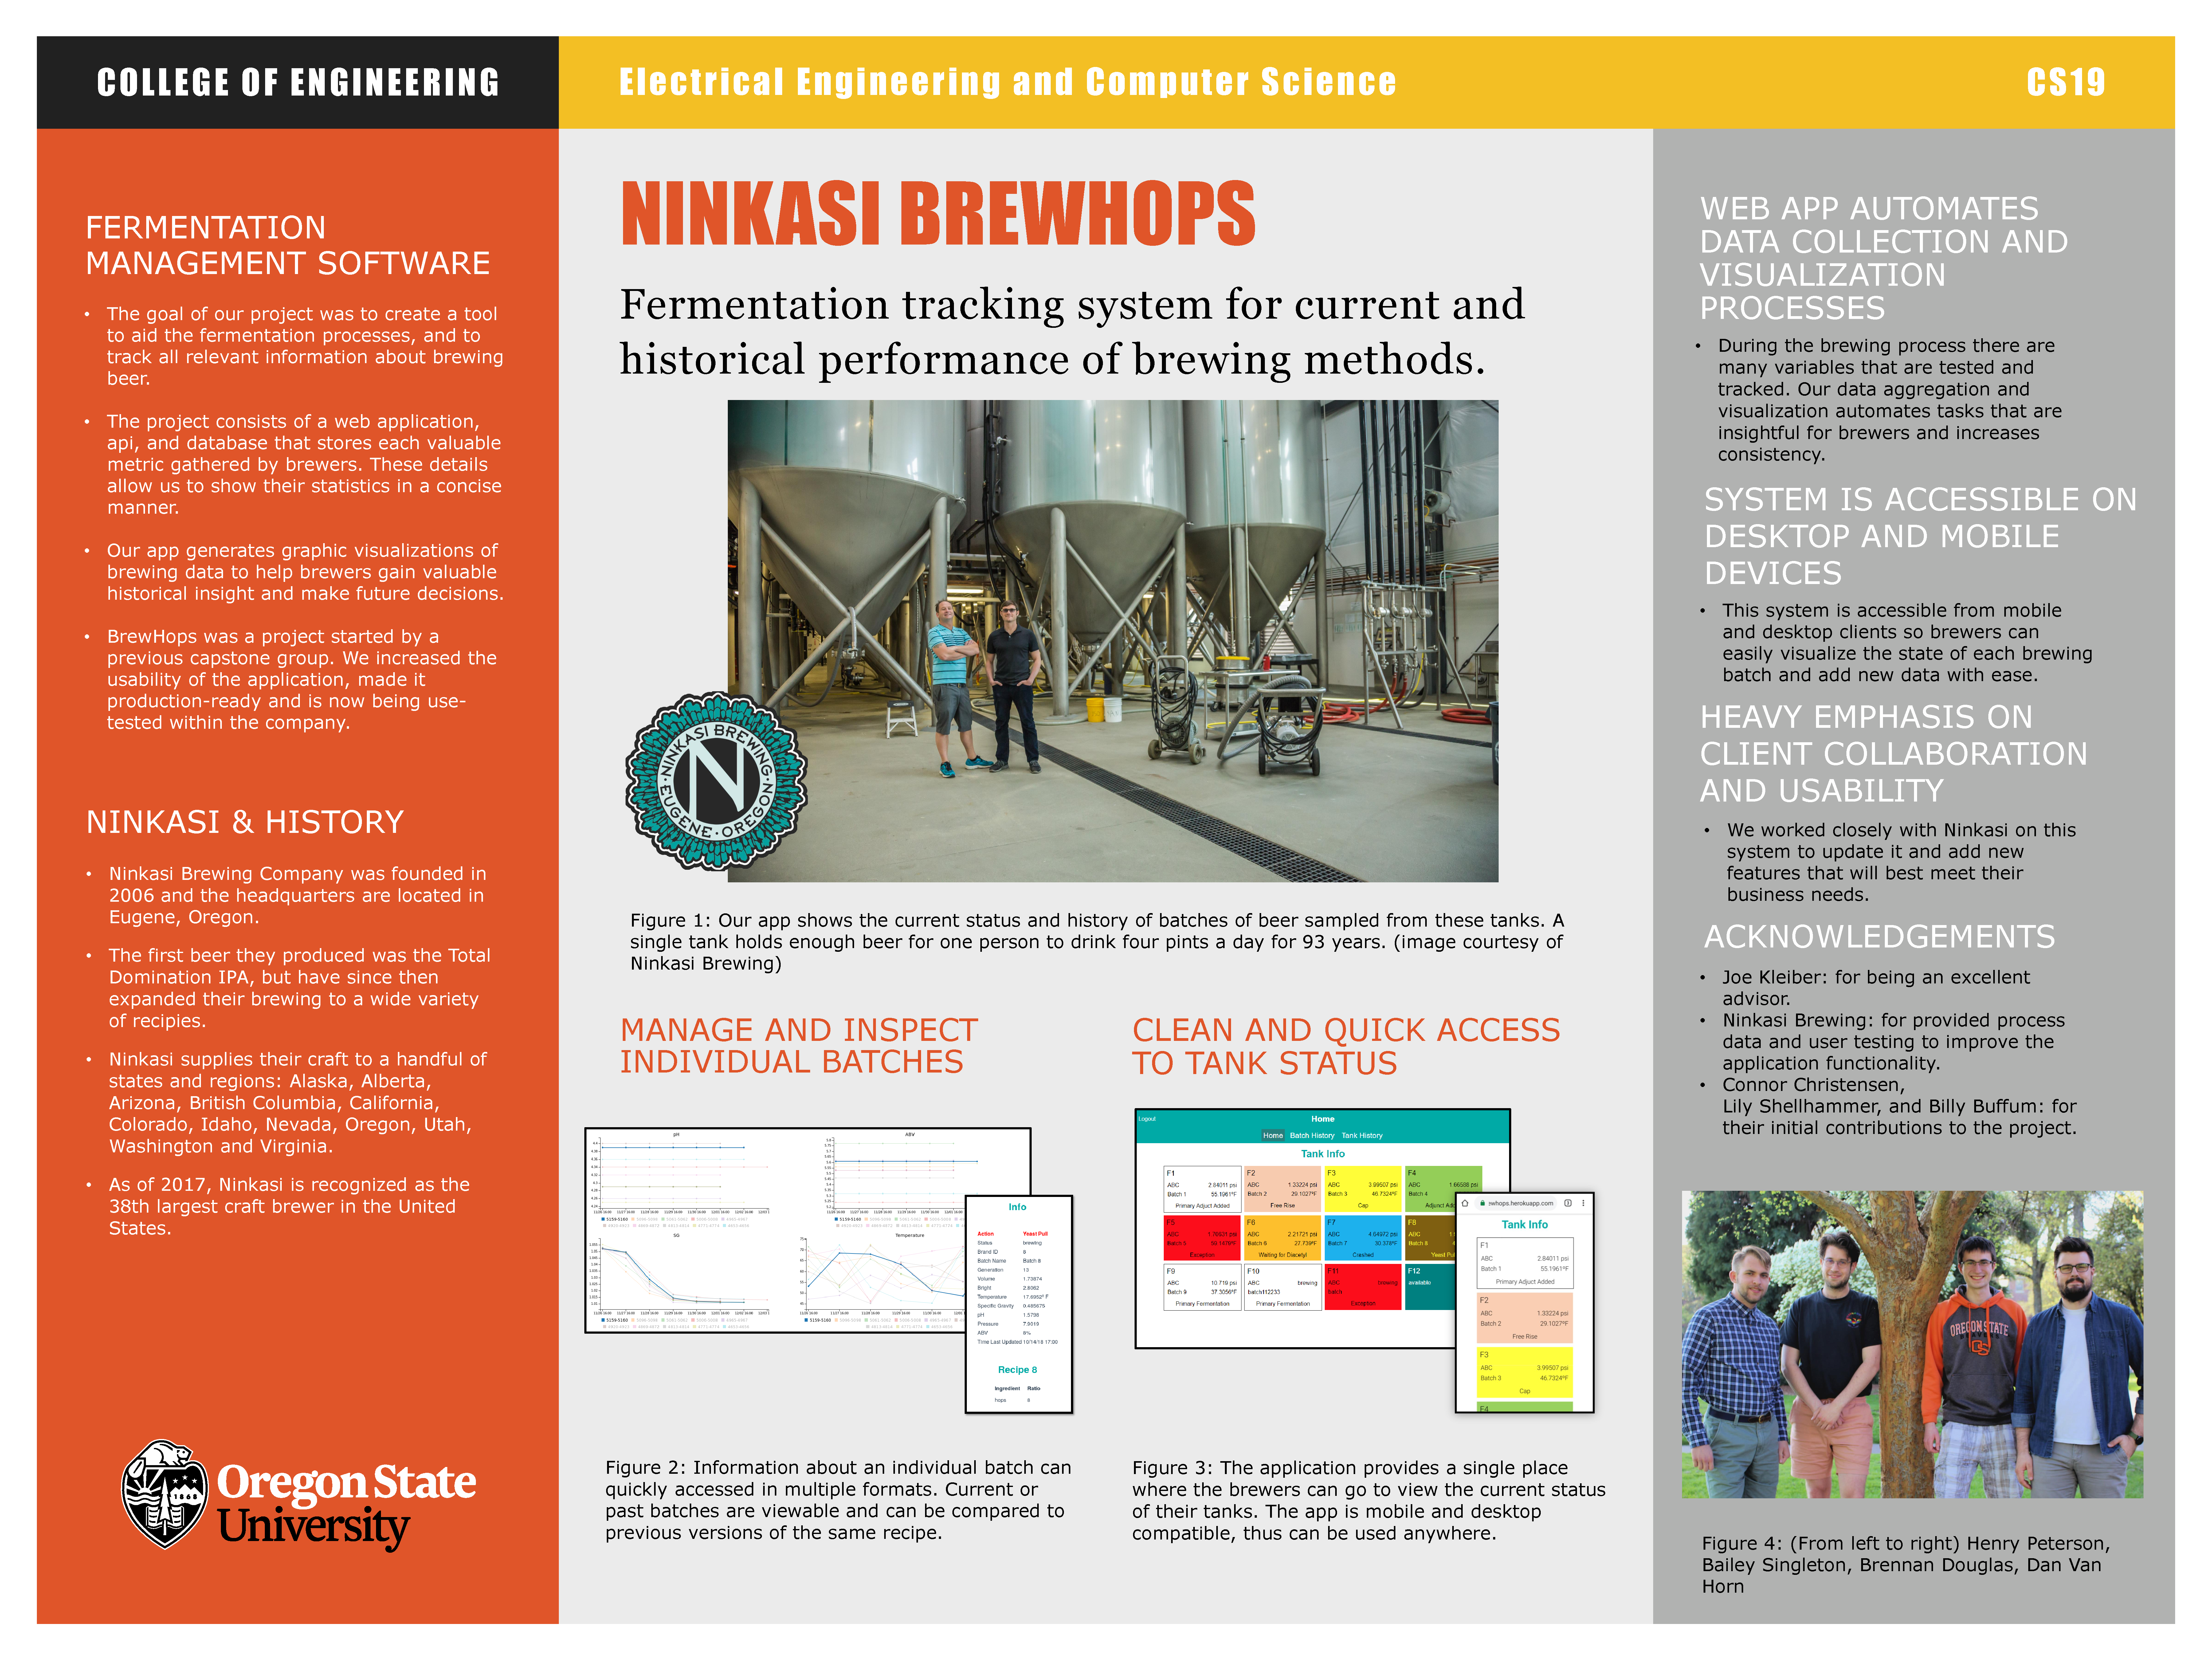
\includegraphics[clip, trim=0cm 0cm 0cm 0cm, width=0.8\paperheight]{Group19_BrewHops-poster_expo_48x36_eecs_final_v2.pdf}}
    \end{center}
\end{landscape}

%\section{Expo Poster}
%See next page.
%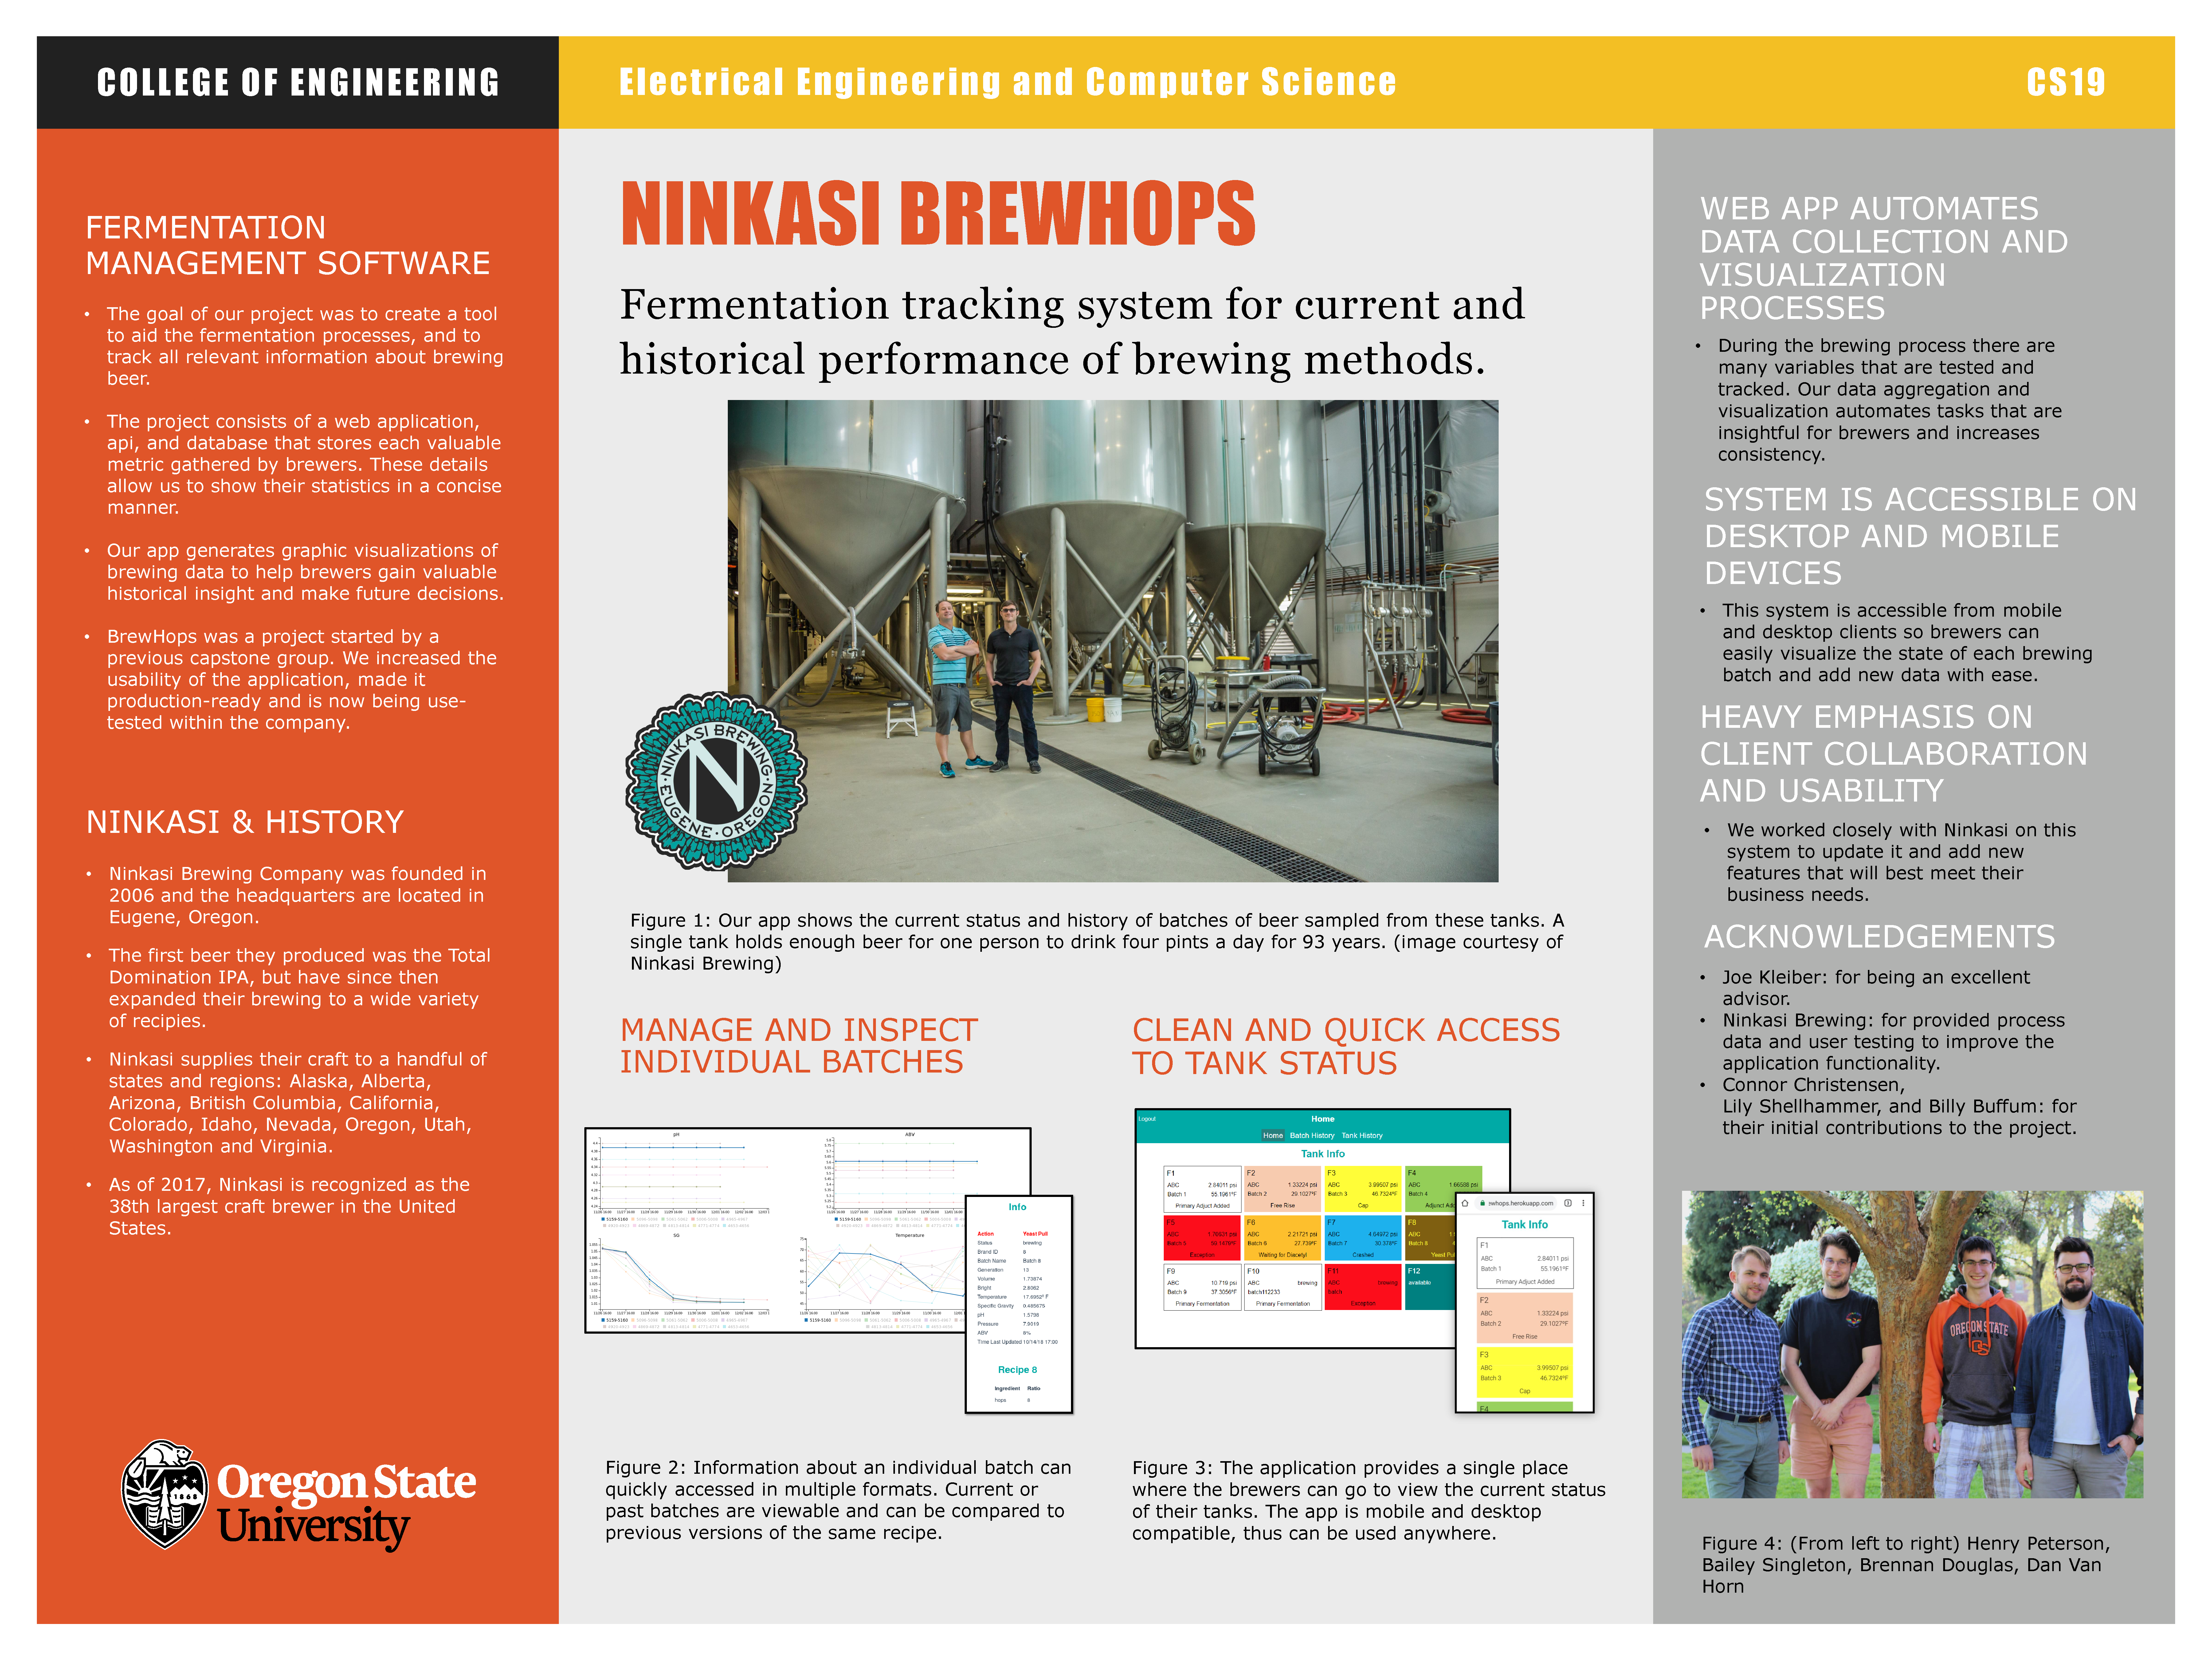
\includepdf[pages=1, landscape]{Group19_BrewHops-poster_expo_48x36_eecs_final_v2.pdf}

\newpage
\section{Project Documentation}

\subsection{API Documentation}

\subsubsection{Purpose of API}
The general purpose of the API is to keep track of how a batch of beer is being brewed over time. There are some peripheral information pieces such as employees that are working on the system, the tanks that the batches are being brewed in, actions associated with those tanks, and the recipes for a brew.

\subsubsection{Requirments}
\begin{itemize}
    \item npm
    \item Docker
    \item Docker Compose
\end{itemize}

\subsubsection{Startup}
Both development and production environments require the use of a .env file to get environment variables. This .env file should never be committed, you can rename the example.env file in the project to .env and it will work. It contains the following environment variables

\begin{itemize}
    \item PGUSER --- The PostGres username
    \item PGDATABASE --- The PostGres database name
    \item PGPASSWORD --- The PostGres database password
    \item PORT --- The Port that the database connects to
\end{itemize}

\noindent
For more information on the PG environment variables, check out the official postgres docker container docs (\href{https://hub.docker.com/_/postgres/}{https://hub.docker.com/_/postgres/}).

\subsubsection{Development}
\begin{enumerate}
    \item 'cp example.env .env' will enable the default configuration.
    \item 'npm i' will install all of the dependencies.
    \item Run 'npm run watch-ts' in a different terminal, this will trigger the typescript compiler to watch the source files for changes and re-transpile them.
    \item 'npm run build-images' will run 'docker-compose', build new images, and run the api.
    \item 'npm run dev' will run 'docker-compose', and run the api.
\end{enumerate}

\subsubsection{Postman}
The postman collection at the root of this repo contains documentation for all of the avaiable api endpoints.

\subsubsection{Test Data}
Once the application has started the init-live endpoint needs to be hit to initialize the test data for the application. Once hit (after success) this can take between 10 seconds to a minute to load all of the data. The following curl command can be used to hit the endpoint:
\begin{verbatim}
    curl -X POST http://localhost:3000/init-live
\end{verbatim}
Or, postman could also be used to hit this endpoint instead of the curl command.

\subsubsection{Checking the database (manually)}
To connect to the docker container and interact directly with the database, follow these steps. {\bf NOTE}: for the automatic psql instance check the npm commands section.
\begin{enumerate}
    \item Start up the postgreSQL docker container if it is not already running
    \item Open up a terminal window
    \item 'docker ps' to get the name of the running DB docker container
    \item 'docker exec -it {name of DB container} bash -l'
    \item 'psql -U {PGUSER} -d {database name}'
\end{enumerate}

\noindent
You should now be logged into the psql program on the docker container.

A few things to note:
\begin{itemize}
    \item every line must either start with a {\textbackslash} or end with a ;
    \begin{itemize}
        \item eg. \textbackslash dt shows all database tables
        \item eg. SELECT * FROM actions; selects everything from the actions table
    \end{itemize}
    \item \textbackslash q to quit the psql shell
    \item exit to exit the docker container
\end{itemize}

\subsubsection{npm commands}
\begin{itemize}
    \item {\bf dev}: starts the development docker environment. This mounts the project to the docker container and then runs nodemon. For this to work, your local node version (the one used to run 'npm i') must be version 11 as well.
    \item {\bf build-images}: rebuilds the dockerfiles that are defined in the docker compose file.
    \item {\bf dev-psql}: this automatically connects you with a psql instance to the development database (only if running).
    \item {\bf test}: runs the current tests.
\end{itemize}


\subsection{Web Application}
A web app to allow ninkasi brewing to better track and manage brewery data

\subsubsection{Build Setup}
\begin{minted}[
    xleftmargin=18pt,
    linenos,
    autogobble,
    breaklines,
]{bash}
    # install dependencies
    npm install
    
    # serve with hot reload at localhost:8080
    npm run dev
    
    # build for production with minification
    npm run build
    
    # build for production and view the bundle analyzer report
    npm run build --report
\end{minted}

\newpage
\section{Recommended Technical Resources for Learning More}
One aspect we looked at when choosing the various technologies we used was the amount of support and documentation they provided. All of the following were be helpful in understanding the specific section of the project they pertain to.
\begin{itemize}
    \item Database\\
        PostgreSQL Documentation: \url{https://www.postgresql.org/docs/}
    \item Server\\
        Express.js Documentation: \url{https://expressjs.com/en/api.html}
    \item Language\\ 
        Typescript Documentation: \url{https://www.typescriptlang.org/docs/home.html}
    \item Frontend\\ 
        Vue.js Documentation: \url{https://vuejs.org/v2/api/}
    \item DevOps\\ 
        Docker Documentation: \url{https://docs.docker.com/}
\end{itemize}

Our best resource for understanding the brewing process and tracking fermentation data was our client themselves, Joe Kleiber.

\newpage
\section{Conclusion and Reflections}
\subsection{Brennan Douglas}
The project gave me the opportunity to work a lot more with JavaScript and Typescript than I traditionally get to at work.  This meant I got to work in a fully JavaScript environment and learn the basic practices that go along with that.  I also got to use Docker which I am always fond of as it simplifies the development process and gives a very clear understanding of what is required to run the project as it all has to be clearly stated in one or two places.

As for what I learned on the non-technical side, it was nice to have more hands on experience with project planning from the very start.  I have had experience previously but it has only been on one or two projects.  Using a task board to plan and allocate specific tasks to specific people helped us a lot keep the work divided and under control so no one person was shouldering half the work.  This is part of project management as well, which as a team we all had a say in during our weekly meetings.  We keep a pace such that we would formally meet up once a week and redivide new work as we had completed the other weeks work.  This was only possible because we correctly broke down the tasks to a proper size.

This team only reinforced in me that teamwork on projects is amazing when it is well planned and everyone has an equal stake.  Communication throughout the team was strong and quick which allowed non-technical blockers to be almost non-existent.  If I could do this all over again, the only thing that I would change are some technical details.  Specifically, our front-end framework.  I would have preferred to use a more state based approach to our single page application, ideally in the form of React instead of Vue.

\subsection{Dan Van Horn}
This project offered me an opportunity to better learn Vue as a front end framework and rank it among those I'd like to use in the future. I had some experience before translating small projects from normal Javascript to Typescript, but this project gave me much more experience that I can take directly into industry.

On the non-technical and project management side, this project was a great chance to work on creating a long term plan and seeing it come to fruition. We rarely found ourselves behind if problems arose, because we heavily prioritized our planning phase. A good plan requires allocation of tasks, and the project was an opportunity to do this. Both of these skills are directly transferable to industry.

I had a really great team that got along fairly well. We felt comfortable enough to talk through any issues or disagreements we had. I know some teams aren't always so good together, so the communication skills I learned in our team meetings will serve me well in the future. 

If I could do the project again, I would have elected to use a different UI framework for the front-end. I think, in some ways, we exceeded expectations and could have taken on a few more ambitious goals like completely re-writing the front-end.
\subsection{Henry Peterson}
Some of the best technical knowledge I gained was about backend development. In most of the projects I've worked on before, the backend was already in place and was just something I interacted with. Seeing the process of refactors and updates to our backend made the process make more sense to me.

Working with a client was an important non-technical skill for me. Typically school projects give little thought to how a non-computer science individual would interact with the result. Having to explain our process and reasoning to our client gave me a real-world taste of that and how being lazy could lead to confusion.

Communication is maybe the most important part of working in a group. I've known this before, but the weight associated with the project really cemented it. In the fall, we were relatively disorganized and didn't communicate with our client as often as we should've. I'm very glad the we sat down, discussed, and improved our communication for the winter. I believe it was instrumental to the success of our project.

If I could do this project again, I would've like to use a different front end technology. It was very nice to have it already partially implemented, but for some of my tasks like testing, it presented unseen difficulties. It was impossible to see from the planning stages, but given the information I have know, that what I would change.
\subsection{Bailey Singleton}
This project let me expand my technical skills in many areas. Most importantly was about the development of the backend and server setup. It was mystifying on how one would set up deployment and getting a server to deploy automatically. Using tools like Now and the Heroku database made this process very simple. 

Working with a client was a skill that was something that I had to learn to handle effectively. It is much easier to talk to someone who already knows the technical details, so I would not have to relay the information in layman's terms. When the client wanted something, I had to take what they said and see how it translated back into the code. 

Project work is takes a lot of time and effort that one doesn't see with normal school work. The time is split into different ways, and it doesn't ever really feel like the project or task is finished. Unlike with homework, there is definitely a point when the job is done. With managing a project, a lot of the success comes in the form of how well the members communicate with one another. Poor communication leads to wasted time that could be spent improving the project. This goes with working in a team on any sort of goal.

If I could do it all over again, it would be in the front end development. Starting with a project that had some work done already made it hard to figure out exactly what was going on, as different minds had different ideas. I would probably go a completely different direction, instead of using Vue I would use React for our frontend. Other than that, there is not much I would change about the project.



\section{Appendix}
\subsection{Essential Code Listings}
Converting the project to Typescript gave us the opportunity to explicitly declare interfaces that declare function return types, parameters and object properties. This was instrumental when the team used these functions because the IDE would show an error if there was a type mismatch. Shown below are the interfaces for our Data Access layer, which defines all interactions with our database.
\begin{minted}
[
frame=lines,
framesep=2mm,
baselinestretch=1.2,
fontsize=\footnotesize
]{js}
export interface ICrudController {
  tableName: () => string;
  connect: () => Promise<void>;
  disconnect: () => Promise<void>;
  create: (columns: any, conditions: any, escaped: any[]) => Promise<QueryResult>;
  createInTable: (
    columns: any,
    table: any,
    conditions: any,
    escaped: any[]
  ) => Promise<QueryResult>;
  read: (columns: string, conditions: string, escaped: any[]) => Promise<QueryResult>;
  readById: (escaped: any) => Promise<QueryResult>;
  readByUsername: (username: any) => Promise<QueryResult>;
  readInTable: (columns: any, table: any, conditions: any, escaped: any[]) => Promise<QueryResult>;
  update: (columns: any, conditions: any, escaped: any[]) => Promise<QueryResult>;
  // tslint:disable-next-line:no-reserved-keywords
  delete: (conditions: any, escaped: any[]) => Promise<QueryResult>;
  deleteById: (escaped: any[]) => Promise<QueryResult>;
  deleteInTable: (table: any, conditions: any, escaped: any[]) => Promise<QueryResult>;
}

export interface IPostgresController extends ICrudController {
  splitObjectKeyVals: (obj: any) => any;
  buildQueryByID: (key: string, value: string) => string;
  buildUpdateString: (keys: any) => any;
}
\end{minted}

The following code is the refactored version of a very large chain of requests from the original application. It contains a lot of logic and even now, it takes a while to understand. The original code however, was nested six layers deep and was incredibly difficult to read. This code is objectively easier to reason about and understand.

\begin{minted}
[
frame=lines,
framesep=2mm,
baselinestretch=1.2,
fontsize=\footnotesize
]{js}
try {
  const batchResponse = await this.$http.get(`${process.env.API}/batches`);
  const tanksResponse = await this.$http.get(`${process.env.API}/tanks`);
  const tasksResponse = await this.$http.get(`${process.env.API}/tasks`);
  const actionsResponse = await this.$http.get(`${process.env.API}/actions`);
  const recipeResponse = await this.$http.get(`${process.env.API}/recipes`);
  for (const tankInfo of tanksResponse.data) {
    // create a temporary tank for us to fill with data
    const tank: ITank = {
      // keep track of tank id for searching
      id: tankInfo.id,
      // keep track of tank name for displaying
      name: tankInfo.name,
      status: tankInfo.status
    };
    for (const batch of batchResponse.data) {
      // if our batches tankID matches our tankID
      if (batch.tank_id === tank.id) {
        tank.batch = {};
        // add in our batchesID to the tank info box
        tank.batch.id = batch.id;
        tank.batch.name = batch.name;
        // add the recipeID to the tank info box
        tank.recipe_id = batch.recipe_id;
      }
    }
    for (const recipeHistory of recipeResponse.data) {
      if (tank.recipe_id === recipeHistory.id) {
        tank.airplane_code = recipeHistory.airplane_code;
      }
    }
    if (tank.batch) {
      const versionsResponse = await this.$http.get(
        `${process.env.API}/versions/batch/${tank.batch.id}`
      );
      // keep track of most recent date with a starting low value
      let max = moment('1995-07-29');
      // for every data point we have in a batch
      for (const batchHistory of versionsResponse.data) {
        // if the date is the largest, it is the most recent one
        if (moment(batchHistory.updated_at) > max) {
          max = moment(batchHistory.updated_at);
          tank.pressure = batchHistory.pressure;
          tank.temperature = batchHistory.temperature;
        }
      }
      // find task associated with tank
      for (const task of tasksResponse.data) {
        if (tank.batch.id === task.batch_id) {
          // if task has our batch id
          tank.action_id = task.action_id; // save the asscoiated action
        }
      }
    }
    // find action associated with task
    for (const action of actionsResponse.data) {
      if (tank.action_id === action.id) {
        tank.action = action.name;
        tank.action_id = `action${action.id}`;
      }
    }
    // push data holder to the tanks array
    this.tanks.push(tank);
  }
  this.tanks.sort(this.sortTanks);
\end{minted}

% bibliography
\nocite{*}%if nothing is referenced it will still show up in refs
\bibliographystyle{IEEEtran}
\bibliography{ref}
%end bibliography

\end{document}
